% Options for packages loaded elsewhere
\PassOptionsToPackage{unicode}{hyperref}
\PassOptionsToPackage{hyphens}{url}
\PassOptionsToPackage{dvipsnames,svgnames,x11names}{xcolor}
%
\documentclass[
  12pt,
  oneside]{book}
\usepackage{amsmath,amssymb}
\usepackage{iftex}
\ifPDFTeX
  \usepackage[T1]{fontenc}
  \usepackage[utf8]{inputenc}
  \usepackage{textcomp} % provide euro and other symbols
\else % if luatex or xetex
  \usepackage{unicode-math} % this also loads fontspec
  \defaultfontfeatures{Scale=MatchLowercase}
  \defaultfontfeatures[\rmfamily]{Ligatures=TeX,Scale=1}
\fi
\usepackage{lmodern}
\ifPDFTeX\else
  % xetex/luatex font selection
\fi
% Use upquote if available, for straight quotes in verbatim environments
\IfFileExists{upquote.sty}{\usepackage{upquote}}{}
\IfFileExists{microtype.sty}{% use microtype if available
  \usepackage[]{microtype}
  \UseMicrotypeSet[protrusion]{basicmath} % disable protrusion for tt fonts
}{}
\makeatletter
\@ifundefined{KOMAClassName}{% if non-KOMA class
  \IfFileExists{parskip.sty}{%
    \usepackage{parskip}
  }{% else
    \setlength{\parindent}{0pt}
    \setlength{\parskip}{6pt plus 2pt minus 1pt}}
}{% if KOMA class
  \KOMAoptions{parskip=half}}
\makeatother
\usepackage{xcolor}
\usepackage{longtable,booktabs,array}
\usepackage{calc} % for calculating minipage widths
% Correct order of tables after \paragraph or \subparagraph
\usepackage{etoolbox}
\makeatletter
\patchcmd\longtable{\par}{\if@noskipsec\mbox{}\fi\par}{}{}
\makeatother
% Allow footnotes in longtable head/foot
\IfFileExists{footnotehyper.sty}{\usepackage{footnotehyper}}{\usepackage{footnote}}
\makesavenoteenv{longtable}
\usepackage{graphicx}
\makeatletter
\def\maxwidth{\ifdim\Gin@nat@width>\linewidth\linewidth\else\Gin@nat@width\fi}
\def\maxheight{\ifdim\Gin@nat@height>\textheight\textheight\else\Gin@nat@height\fi}
\makeatother
% Scale images if necessary, so that they will not overflow the page
% margins by default, and it is still possible to overwrite the defaults
% using explicit options in \includegraphics[width, height, ...]{}
\setkeys{Gin}{width=\maxwidth,height=\maxheight,keepaspectratio}
% Set default figure placement to htbp
\makeatletter
\def\fps@figure{htbp}
\makeatother
\usepackage{soul}
\setlength{\emergencystretch}{3em} % prevent overfull lines
\providecommand{\tightlist}{%
  \setlength{\itemsep}{0pt}\setlength{\parskip}{0pt}}
\setcounter{secnumdepth}{5}
\usepackage{tikz}
\usepackage{tkz-euclide}
\usepackage{pgfplots}
\usetikzlibrary{decorations}
\usetikzlibrary{shapes.geometric}
\usetikzlibrary{arrows.meta}
\usetikzlibrary{arrows,calc}
\pgfplotsset{compat=newest}
\pgfplotsset{plot coordinates/math parser=false}
\usetikzlibrary{intersections}
\usetikzlibrary{decorations.pathreplacing}
\usepgflibrary{patterns}
\usetikzlibrary{patterns}
\usepgfplotslibrary{fillbetween}
\usepackage{tikz}
\usepackage{pgfplots}
\usepackage{pgf,tikz,pgfplots}
\pgfplotsset{compat=1.15}
\usepackage{mathrsfs}
\usetikzlibrary{arrows}
\usetikzlibrary{patterns}
\usepackage{tikz}
\usepackage{pgfplots}
\ifLuaTeX
  \usepackage{selnolig}  % disable illegal ligatures
\fi
\usepackage[]{natbib}
\bibliographystyle{plainnat}
\IfFileExists{bookmark.sty}{\usepackage{bookmark}}{\usepackage{hyperref}}
\IfFileExists{xurl.sty}{\usepackage{xurl}}{} % add URL line breaks if available
\urlstyle{same}
\hypersetup{
  pdftitle={Managerial Economics},
  pdfauthor={© Prof.~Dr.~Stephan Huber (Stephan.Huber@hs-fresenius.de)},
  colorlinks=true,
  linkcolor={red},
  filecolor={Maroon},
  citecolor={Blue},
  urlcolor={blue},
  pdfcreator={LaTeX via pandoc}}

\title{Managerial Economics}
\usepackage{etoolbox}
\makeatletter
\providecommand{\subtitle}[1]{% add subtitle to \maketitle
  \apptocmd{\@title}{\par {\large #1 \par}}{}{}
}
\makeatother
\subtitle{Lecture Notes}
\author{© Prof.~Dr.~Stephan Huber (\href{mailto:Stephan.Huber@hs-fresenius.de}{\nolinkurl{Stephan.Huber@hs-fresenius.de}})}
\date{Last compiled on 21 June, 2024}

\usepackage{amsthm}
\newtheorem{theorem}{Theorem}[chapter]
\newtheorem{lemma}{Lemma}[chapter]
\newtheorem{corollary}{Corollary}[chapter]
\newtheorem{proposition}{Proposition}[chapter]
\newtheorem{conjecture}{Conjecture}[chapter]
\theoremstyle{definition}
\newtheorem{definition}{Definition}[chapter]
\theoremstyle{definition}
\newtheorem{example}{Example}[chapter]
\theoremstyle{definition}
\newtheorem{exercise}{Exercise}[chapter]
\theoremstyle{definition}
\newtheorem{hypothesis}{Hypothesis}[chapter]
\theoremstyle{remark}
\newtheorem*{remark}{Remark}
\newtheorem*{solution}{Solution}
\begin{document}
\maketitle

{
\hypersetup{linkcolor=}
\setcounter{tocdepth}{2}
\tableofcontents
}
\hypertarget{preface}{%
\chapter*{Preface}\label{preface}}
\addcontentsline{toc}{chapter}{Preface}

\begin{itemize}
\tightlist
\item
  This is work in progress and it will develop during the semester so please check for updates regularly.
\item
  I appreciate you reading it, and I appreciate any comments, but please do not share this document or quote it without asking me.
\item
  This script aims to support my lecture at the HS Fresenius. It is incomplete and no substitute
  for taking actively part in class.
\item
  Do not distribute without permission.
\item
  The lecture notes are available online or you can download it as a \href{https://raw.githubusercontent.com/hubchev/hubchev.github.io/main/me/_main.pdf}{pdf file here}
\end{itemize}

\hypertarget{about-the-author}{%
\section*{About the author}\label{about-the-author}}

\begin{figure}
\centering
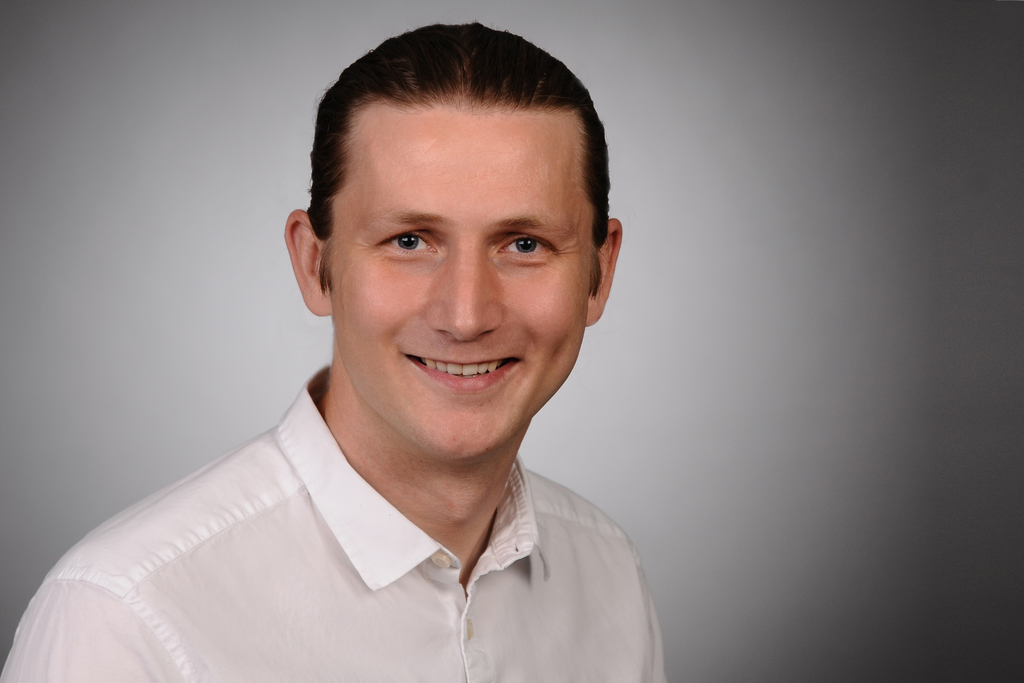
\includegraphics[width=0.25\textwidth,height=\textheight]{fig/huber2.jpeg}
\caption[\label{fig:itsme} Prof.~Dr.~Stephan Huber]{\label{fig:itsme} Prof.~Dr.~Stephan Huber\footnotemark{}}
\end{figure}
\footnotetext{Picture is taken from \url{https://sites.google.com/view/stephanhuber}}

I am a Professor of International Economics and Data Science at HS Fresenius, holding a Diploma in Economics from the University of Regensburg and a Doctoral Degree (summa cum laude) from the University of Trier. I completed postgraduate studies at the Interdisciplinary Graduate Center of Excellence at the Institute for Labor Law and Industrial Relations in the European Union (IAAEU) in Trier. Prior to my current position, I worked as a research assistant to Prof.~Dr.~Dr.~h.c. Joachim Möller at the University of Regensburg, a post-doc at the Leibniz Institute for East and Southeast European Studies (IOS) in Regensburg, and a freelancer at Charles University in Prague.

Throughout my career, I have also worked as a lecturer at various institutions, including the TU Munich, the University of Regensburg, Saarland University, and the Universities of Applied Sciences in Frankfurt and Augsburg. Additionally, I have had the opportunity to teach abroad for the University of Cordoba in Spain and the University of Perugia. My published work can be found in international journals such as the Canadian Journal of Economics and the Stata Journal. For more information on my work, please visit my private homepage at \url{https://hubchev.github.io}.

\textbf{Contact}

\begin{verbatim}
   Hochschule Fresenius für Wirtschaft & Medien GmbH
   Im MediaPark 4c
   50670 Cologne
   
   Office: 4b OG-1 Bü01 (Office hour: Thursday 1-2 p.m.)
   Telefon: +49 221 973199-523
   Mail: stephan.huber@hs-fresenius.de
   Private homepage: www.t1p.de/stephanhuber
   Github: https://hubchev.github.io/
\end{verbatim}

\hypertarget{about-this-course}{%
\section*{About this course}\label{about-this-course}}

\textbf{Workload:}
125 h = 42 h (in-class) + 21 h (guided private study hours) - 62 h (private self-study).

\textbf{Assessment}
Students complete this module with a written exam of 90 minutes. A passing grade in this module is achieved when the overall grade is greater than or equal to 4.0.

\textbf{Learning outcomes:}
After successful completion of the module, students are able to:

\begin{itemize}
\tightlist
\item
  describe how tools of standard price theory, location theory, production theory, and the theory of investment decision can be employed to formulate a decision problem,
\item
  evaluate alternative courses of action and choose among alternatives,
\item
  apply economic concepts and techniques in evaluating strategic business decisions taken by firms,
\item
  apply the knowledge of the mechanics of supply and demand to explain the functioning of markets.
\end{itemize}

\textbf{How to prepare for the exam:}
I am convinced that reading the lecture notes, preparing for class, taking actively part in class, and trying to solve the exercises without going straight to the solutions is the best method for students to

\begin{itemize}
\tightlist
\item
  maximize leisure time and minimize the time needed to prepare for the exam, respectively,
\item
  getting long-term benefits out of the course,
\item
  improve grades, and
\item
  have more fun during lecture hours.
\end{itemize}

\textbf{Literature:}
\citet{Bazerman2017Judgement}, \citet{Hoover2020Introduction}, \citet{Parkin2017Economics}, \citet{Wilkinson2022Managerial}, \citet{Bonanno2017Decision}

\textbf{Content:}

\hypertarget{price-theory}{%
\paragraph*{Price theory}\label{price-theory}}
\addcontentsline{toc}{paragraph}{Price theory}

\begin{itemize}
\tightlist
\item
  the market price of an efficient competitive market and sources of inefficiency
\item
  the impact of supply and demand on the market price
\item
  the output and price decision of a profit maximizing monopolist
\item
  regional market power and price setting
\end{itemize}

\hypertarget{production-and-cost-theory}{%
\paragraph*{Production and cost theory}\label{production-and-cost-theory}}
\addcontentsline{toc}{paragraph}{Production and cost theory}

\begin{itemize}
\tightlist
\item
  output and costs of firms in the short and long run
\item
  optimization under constraints (Lagrangian multiplier)
\item
  cost--volume--profit analysis
\end{itemize}

\hypertarget{location-theory}{%
\paragraph*{Location theory}\label{location-theory}}
\addcontentsline{toc}{paragraph}{Location theory}

\begin{itemize}
\tightlist
\item
  Hotelling's location model
\item
  Thünen's model of agricultural land use
\item
  location fundamentals and agglomeration forces (sharing, matching, learning)
\end{itemize}

\hypertarget{strategic-behaviour-of-firms}{%
\paragraph*{Strategic behaviour of firms}\label{strategic-behaviour-of-firms}}
\addcontentsline{toc}{paragraph}{Strategic behaviour of firms}

\begin{itemize}
\tightlist
\item
  nature, scope, and elements of game theory
\item
  static games (Nash, Cournot, and Bertrand equilibrium)
\item
  limitations
\end{itemize}

\hypertarget{investment-decisions}{%
\paragraph*{Investment decisions}\label{investment-decisions}}
\addcontentsline{toc}{paragraph}{Investment decisions}

\begin{itemize}
\tightlist
\item
  net present value
\item
  internal rate of return
\item
  decision-making under risk
\item
  decision-making under uncertainty
\item
  common pitfalls in investment decisions
\end{itemize}

\hypertarget{about-how-to-learn-and-prepare-for-the-exam}{%
\subsection*{About how to learn (and prepare for the exam)}\label{about-how-to-learn-and-prepare-for-the-exam}}

\begin{figure}
\centering
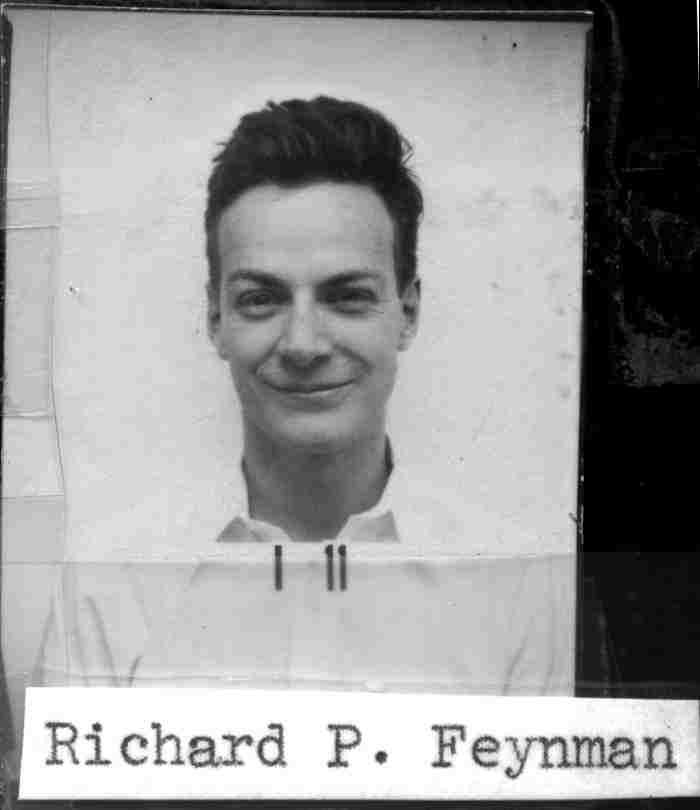
\includegraphics[width=0.25\textwidth,height=\textheight]{fig/Richard-Feynman.jpg}
\caption[\label{fig:feynman} Richard P. Feynman's badge photo from Los Alamos National Laboratory]{\label{fig:feynman} Richard P. Feynman's badge photo from Los Alamos National Laboratory\footnotemark{}}
\end{figure}
\footnotetext{Picture is taken from \url{https://repository.aip.org/islandora/object/nbla\%3A299600}}

Richard P. Feynman:

\begin{quote}
``I don't know what's the matter with people: they don't learn by understanding; they learn by some other way ­ by rote, or something. Their knowledge is so fragile!''
\end{quote}

Stephan Huber:

\begin{quote}
``I agree with Feynman: The key to learning is understanding. However, I believe that there is no understanding without practice, that is, solving problems and exercises by yourself with a pencil and a blank sheet of paper without knowing the solution in advance.''
\end{quote}

\begin{itemize}
\tightlist
\item
  Study the lecture notes, i.e., try to understand the exercises and solve them yourself.
\item
  Study the exercises, i.e., try to understand the logical rules and solve the problems yourself.
\item
  Test yourself with past exams that you will find on ILIAS. The structure of the exam is more or less the same every semester.
\item
  If you have the opportunity to form a group of students to study and prepare for the exam, make use of it. It is great to help each other, and it is very motivating to see that everyone has problems sometimes.
\item
  If you have difficulties with some exercises and the solutions shown do not solve your problem, ask a classmate or contact me. I will do my best to help.
\end{itemize}

\hypertarget{what-is-managerial-economics}{%
\chapter{What is managerial economics?}\label{what-is-managerial-economics}}

\begin{center}\rule{0.5\linewidth}{0.5pt}\end{center}

After successful completion of the module, students are able to:

\begin{itemize}
\tightlist
\item
  Explain what managerial economics is all about.
\item
  Discuss the use of managerial econmics for their private and professional lifes.
\item
  Explain how managerial economics relates to other disciplines of social sciences.
\end{itemize}

\begin{center}\rule{0.5\linewidth}{0.5pt}\end{center}

Well, that's a question that can't be answered definitively. It is whatever you would like it to be. Each instructor may find a slightly different way to define what it is. However, there are some conventions for what many people mean by it. To find out what most people mean by managerial economics, public and general sources like Wikipedia are a good source.\footnote{Usually, it is not a good idea to cite Wikipedia in an academic paper, because everything written down in Wikipedia has to come from some other source. So Wikipedia is usually only a secondary source. However, general definitions of an important topic are sometimes worth citing, as they can be seen as a definition that is at least accepted by a more or less large group of administrators who can make changes to Wikipedia}.

More recent, many people start using ChatGPT for good reasons. \citet{Korinek2023Language} discusses the use of it for academic research. Lets see what ChatGPT and Wikipedia say about managerial economics.

\hypertarget{what-is-managerial-economics-for-chatgpt}{%
\section{What is managerial economics for ChatGPT?}\label{what-is-managerial-economics-for-chatgpt}}

\textbf{Define managerial economics.}

\textbf{ChatGPT:} Managerial economics is the application of economic theories, concepts, and analytical tools to solve managerial problems in business organizations. It involves the study of how economic principles can be applied to make better decisions regarding the allocation of resources, production and consumption of goods and services, pricing strategies, market analysis, and other strategic issues facing firms. The main goal of managerial economics is to provide managers with a framework to analyze business problems and make informed decisions that will maximize the firm's profits and shareholder value. It is an interdisciplinary field that draws from economics, finance, accounting, statistics, and other related fields to help managers understand the economic environment in which they operate and make effective decisions.

\textbf{What distinguishes managerial economics from Microeconomics and Macroeconomics?}

\textbf{ChatGPT:} Managerial economics is closely related to both microeconomics and macroeconomics, but it differs from these two branches of economics in several ways:

\begin{enumerate}
\def\labelenumi{\arabic{enumi}.}
\item
  Scope: Microeconomics focuses on the behavior of individual economic agents, such as households and firms, while macroeconomics focuses on the behavior of the economy as a whole, including variables such as aggregate output, employment, and inflation. Managerial economics, on the other hand, focuses on the decision-making behavior of individual firms, and how they interact with the market and other firms.
\item
  Purpose: The purpose of microeconomics is to study the allocation of resources among different uses and the interactions of individual agents in the market, while macroeconomics is concerned with the overall performance of the economy. Managerial economics, on the other hand, is concerned with applying economic principles to solve managerial problems in business organizations, such as pricing strategies, cost analysis, and production decisions.
\item
  Analysis: Microeconomics uses mathematical and graphical models to analyze the behavior of individual agents in the market, while macroeconomics uses aggregate economic data to study the overall performance of the economy. Managerial economics, however, uses both microeconomic and macroeconomic tools and techniques to analyze and solve specific managerial problems.
\item
  Perspective: Microeconomics takes the perspective of an individual economic agent, while macroeconomics takes the perspective of the entire economy. Managerial economics, on the other hand, takes the perspective of the manager and the firm, and how they can use economic principles to make better decisions.
\end{enumerate}

\emph{In summary, while managerial economics draws from both microeconomics and macroeconomics, it focuses on the specific issues facing firms and their decision-making behavior, making it distinct from these other two branches of economics.}

\hypertarget{what-is-managerial-economics-for-wikipedia}{%
\section{What is managerial economics for Wikipedia?}\label{what-is-managerial-economics-for-wikipedia}}

Read \url{https://en.wikipedia.org/wiki/Managerial_economics}

\hypertarget{simple-definition-of-managerial-economics}{%
\section{Simple definition of managerial economics}\label{simple-definition-of-managerial-economics}}

To me managerial economics is economics for managers. That means, any sort of method, information, and knowledge from economic research that can help managers somehow in making good decisions and achieve their goals can be considered to be part of managerial economics. So, now we can discuss what \emph{economics} is all about and what therein can be helpful to managers.

\hypertarget{what-is-economics}{%
\section{What is economics?}\label{what-is-economics}}

All economic questions arise because we want more than we can get. Our inability to satisfy all our wants is called scarcity and because of scarcity, we must make choices that depend on the incentives we face. An incentive is a reward that encourages or a penalty that discourages an action.

Economics is a social science, and as in all social sciences, many of the terms used in it are poorly defined. The following quotes can demonstrate that:

\begin{quote}
John Maynard Keynes (1883-1946): ``The theory of economics does not furnish a body of settled conclusions immediately applicable to policy. It is a method rather than a doctrine, an apparatus of the mind, a technique of thinking, which helps it possessors to draw correct conclusions.'' \citet{Keynes1921Introduction}
\end{quote}

\begin{quote}
Alfred Marshall (1842-1924): ``Economics is a study of mankind in the ordinary business of life; it examines that part of individual and social action which is most closely connected with the attainment and with the use of the material requisites of wellbeing.'' \citet[p.~1]{Marshall2009Principles}
\end{quote}

\begin{quote}
Gary S. Becker (1930-2014): ``Economics is all about how people make choices. Sociology is about why there isn't any choice to be made.'' \citet[p.~233]{Becker1960Economic}
\end{quote}

\begin{quote}
\citet[p.~4]{Colander2006Economics}: ``Economics is the study of how human beings coordinate their wants and desires, given the decision-making mechanisms, social customs, and political realities of the society.''
\end{quote}

\begin{quote}
\citet[p.~2]{Parkin2012Economics}: ``Economics is the social science that studies the choices that individuals, businesses, governments, and entire societies make as they cope with scarcity and the incentives that influence and reconcile those choices.''
\end{quote}

\begin{quote}
\citet[p.~5.]{Gwartney2006Microeconomics}: ``{[}E{]}conomics is the study of human behavior, with a particular focus on human decision making.''
\end{quote}

\begin{quote}
\citet[p.~222]{Backhouse2009Retrospectives}: ``{[}E{]}conomics is apparently the study of the economy, the study of the coordination process, the study of the effects of scarcity, the science of choice, and the study of human behavior.''
\end{quote}

\begin{quote}
\citet[ch.~1]{Greenlaw2022Principles}: Economics seeks to solve the problem of scarcity, which is when human wants for goods and services exceed the available supply. A modern economy displays a division of labor, in which people earn income by specializing in what they produce and then use that income to purchase the products they need or want. The division of labor allows individuals and firms to specialize and to produce more for several reasons: a) It allows the agents to focus on areas of advantage due to natural factors and skill levels; b) It encourages the agents to learn and invent; c) It allows agents to take advantage of economies of scale. Division and specialization of labor only work when individuals can purchase what they do not produce in markets. Learning about economics helps you understand the major problems facing the world today, prepares you to be a good citizen, and helps you become a well-rounded thinker.
\end{quote}

\begin{quote}
\citet[p.~222]{Backhouse2009Retrospectives}: ``Perhaps the definition of economics is best viewed as a tool for the first day of principles classes but otherwise of little concern to practicing economists.''
\end{quote}

\begin{quote}
Jacob Viner (1892-1970): ``Economics is what economists do.'' \citet[p.~222]{Backhouse2009Retrospectives}
\end{quote}

\begin{quote}
\citet[p.~2]{Parkin2012Economics}: ``Microeconomics is the study of the choices that individuals and businesses make, the way these choices interact in markets, and the influence of governments. {[}\ldots{]} Macroeconomics is the study of the performance of the national economy and the global economy.''
\end{quote}

Although many textbook definitions are quite similar in many ways, the
lack of agreement on a clear-cut definition of economics does not really matter and does not necessarily pose a problem as

\begin{quote}
``{[}E{]}conomists are generally guided by pragmatic considerations of what works or by methodological views emanating from various sources, not by formal definitions.'' \citet[p.~231]{Backhouse2009Retrospectives}
\end{quote}

\textbf{The important questions of economics:}
How do choices end up determining what, where, how, and for whom goods and services get produced? And: When do choices made in the pursuit of self-interest also promote the social interest?

\hypertarget{decision-making-basics}{%
\chapter{Decision making basics}\label{decision-making-basics}}

\begin{center}\rule{0.5\linewidth}{0.5pt}\end{center}

After successful completion of the module, students are able to:

\begin{itemize}
\tightlist
\item
  Make decisions with a great awareness of the nature of the decision and the purpose of making a decision.
\item
  Explain the trade-offs that should be taken into account when making a decision.
\item
  Explain different characteristics of decisions.
\item
  Take advantage of various decision making strategies.
\item
  Explain the rational model of decision making and the concept of the homo economicus.
\item
  Explain the bounded rationality of humans and its implications on their ability to make decisions.
\item
  Apply heuristics to make good decisions.
\end{itemize}

\begin{center}\rule{0.5\linewidth}{0.5pt}\end{center}

\hypertarget{exercises-to-reflect-on-how-we-make-decisions}{%
\section{Exercises to reflect on how we make decisions}\label{exercises-to-reflect-on-how-we-make-decisions}}

\begin{exercise}
\protect\hypertarget{exr:brain-color}{}\label{exr:brain-color}Brain

\begin{figure}
\centering
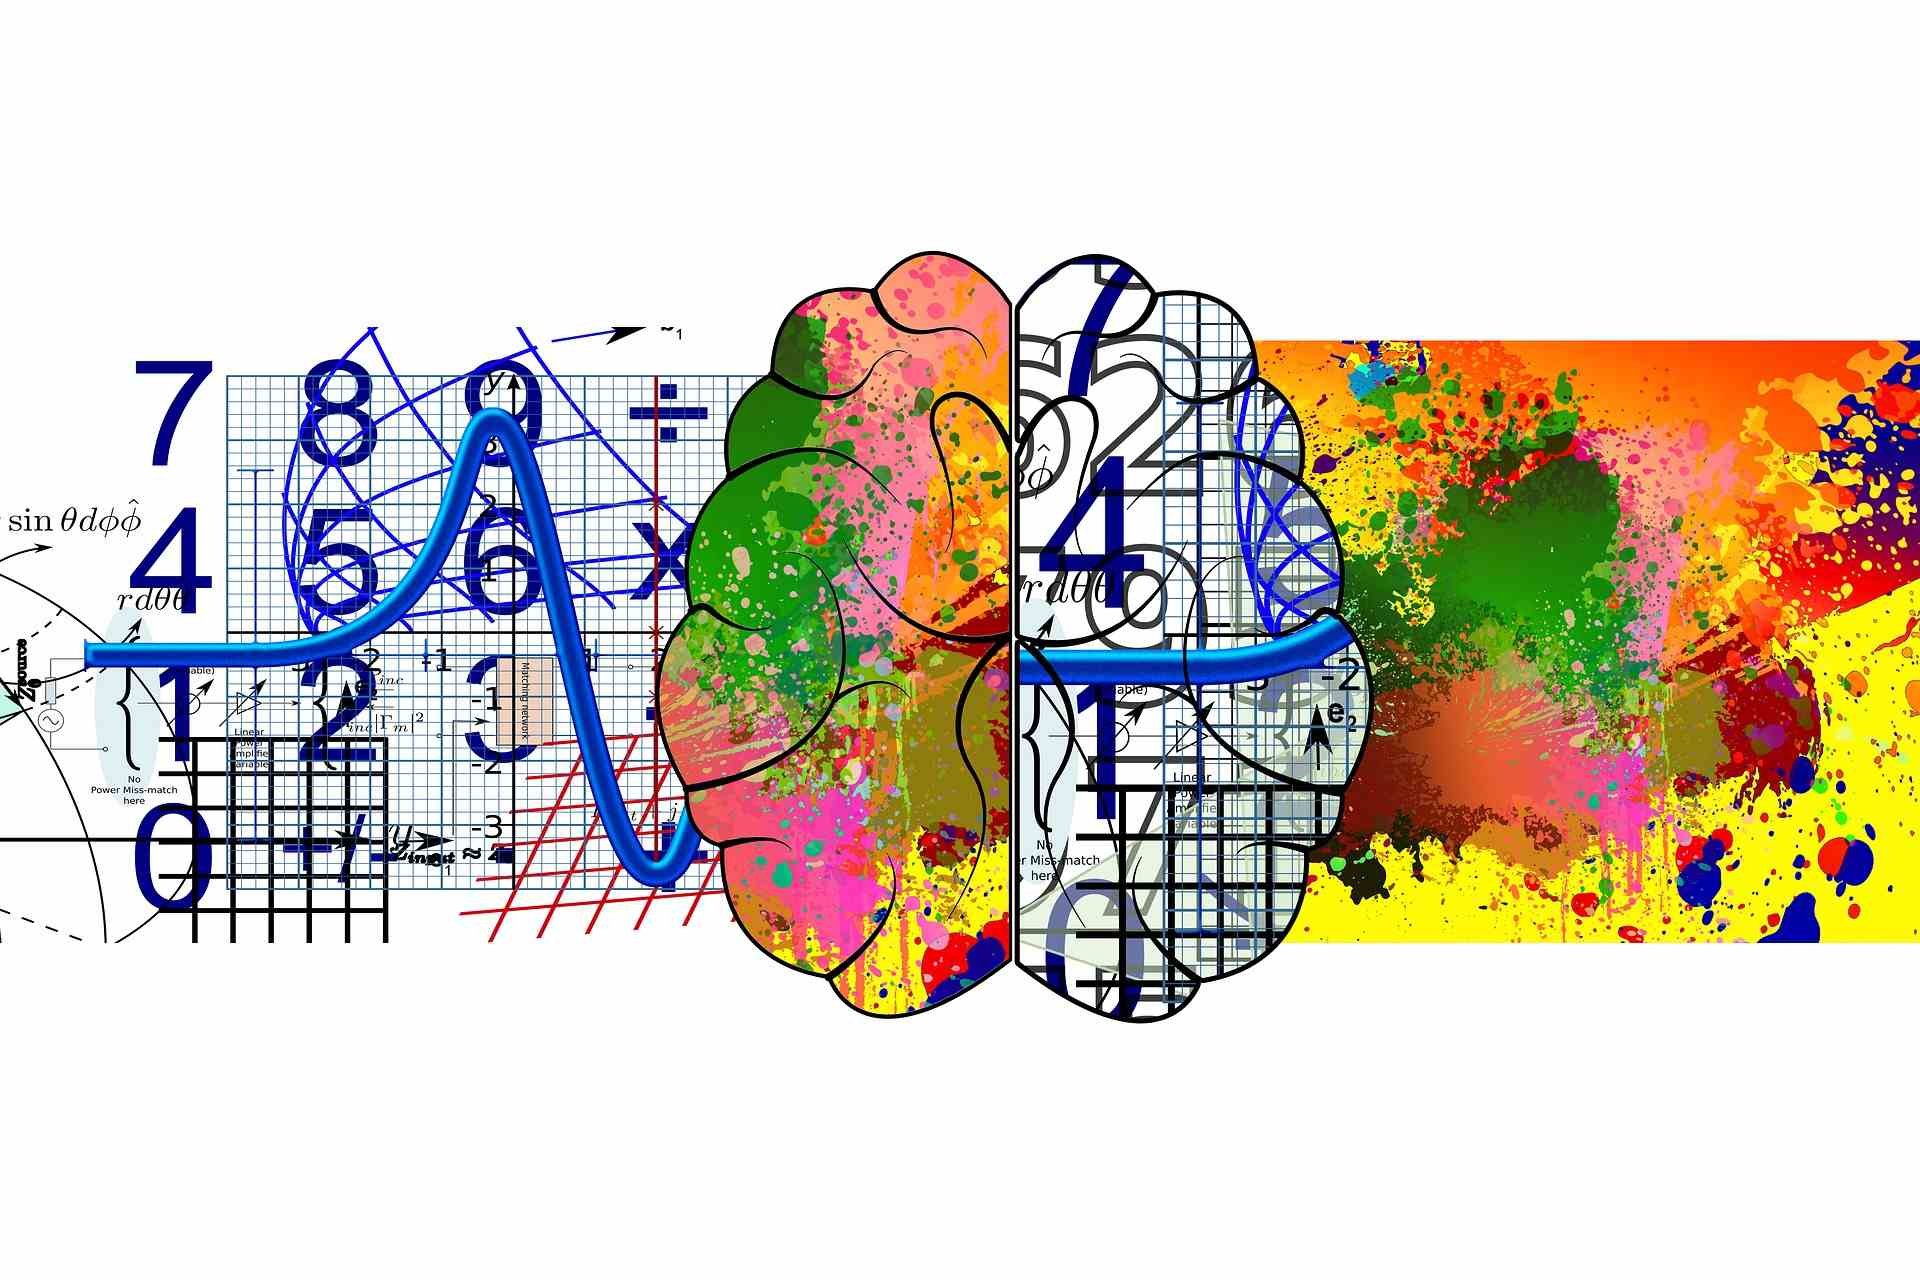
\includegraphics[width=1\textwidth,height=\textheight]{fig/brain-color.jpg}
\caption[\label{fig:brain-color} From data to decision]{\label{fig:brain-color} From data to decision\footnotemark{}}
\end{figure}
\footnotetext{Source: \url{https://pixabay.com/images/id-6671455/}}

Discuss figure \ref{fig:brain-color}. What is the message of the picture?
\end{exercise}

\begin{exercise}
\protect\hypertarget{exr:puzzle}{}\label{exr:puzzle}Solve the puzzles

\begin{enumerate}
\def\labelenumi{\alph{enumi})}
\tightlist
\item
  \textbf{The nine dots problem}
  Connect the dots shown in fugure \ref{fig:9dots} with no more than 4 straight lines without lifting your hand from the paper.
\end{enumerate}

\begin{figure}
\centering

\includegraphics[width=0.15\textwidth,height=\textheight]{fig/9dots.png}
\caption{\label{fig:9dots} The nine dots problem}
\end{figure}

\begin{enumerate}
\def\labelenumi{\alph{enumi})}
\setcounter{enumi}{1}
\tightlist
\item
  \textbf{The tasty cake puzzle} In figure \ref{fig:cake} you see a tasty cake with the nine dots representing strawberries. Cut this cake up with exactly four straight cuts so that each portion of the cake contains just one strawberry on the top.
\end{enumerate}

\begin{figure}
\centering
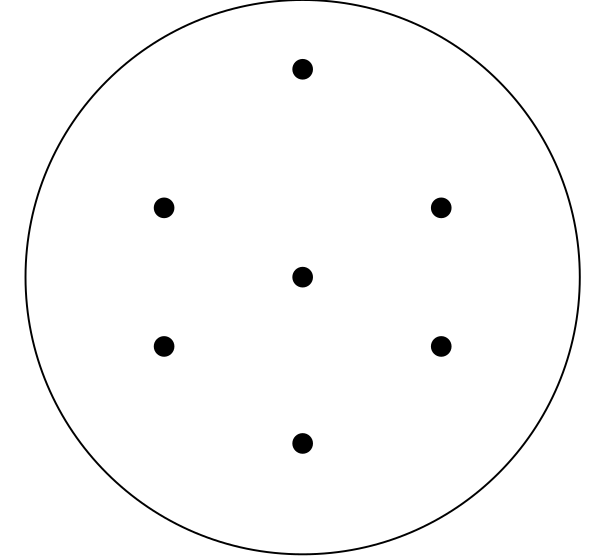
\includegraphics[width=0.25\textwidth,height=\textheight]{fig/cake.png}
\caption{\label{fig:cake} The tasty cake puzzle}
\end{figure}

Reflect on how you tried to solve the puzzles. Did you have a problem solving strategy? How did you come to the right decision? Think of restrictions you imposed on yourself which was not inherent to the problem.
\end{exercise}

\begin{exercise}
\protect\hypertarget{exr:santa}{}\label{exr:santa}

What is the house of Santa Claus?

The house of Santa Claus is an old German drawing game. It goes like this: You have to draw a house in one line where you (a) must start at bottom left (point 1), (b) you are not allowed to lift your pencil while drawing and (c) it is forbidden to repeat a line. During drawing you say: ``Das ist das Haus des Nikolaus'\,'. What do you think is the success-rate of kids who play this game for the first time?

\begin{figure}
\centering
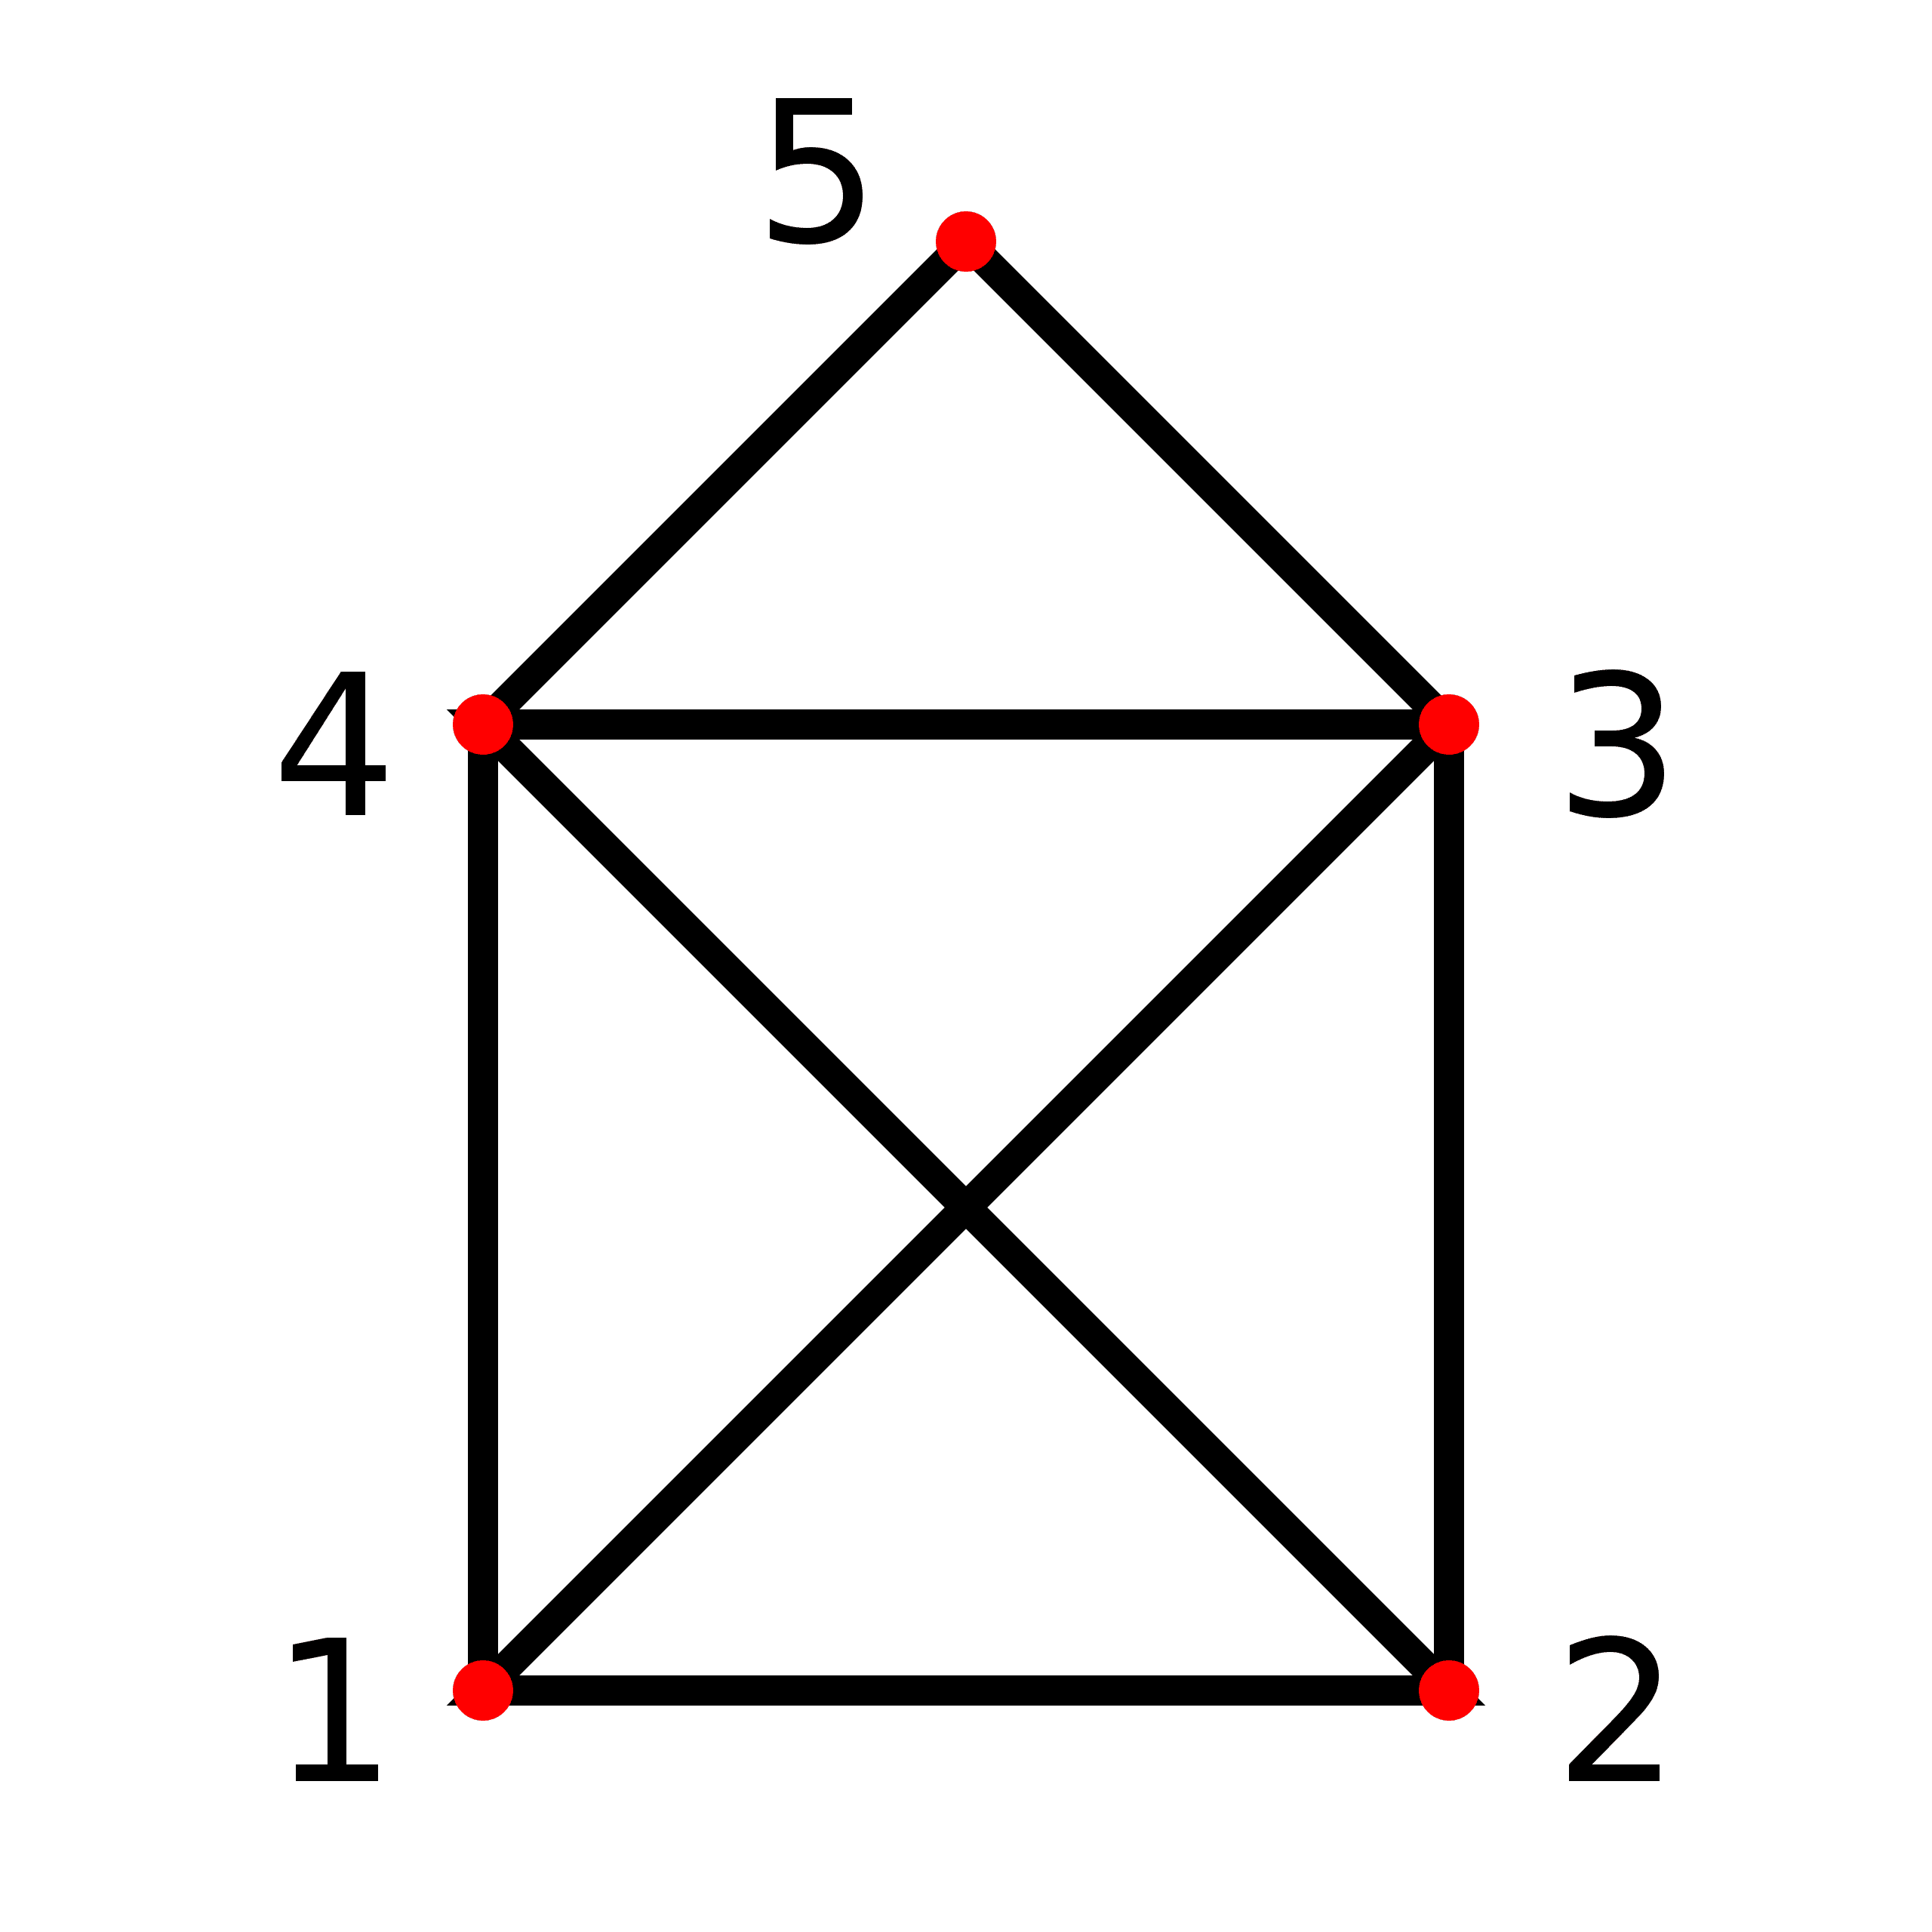
\includegraphics[width=0.25\textwidth,height=\textheight]{fig/nikolaus.png}
\caption{\label{fig:nikolaus} The house of Santa Claus}
\end{figure}

\begin{figure}
\centering

\includegraphics[width=0.2\textwidth,height=\textheight]{fig/pingo666528.png}
\caption{\label{fig:pingo} PINGO}
\end{figure}

Answer the question here:
\url{https://pingo.coactum.de/}
Code: 666528

Please find solution to the exercise \protect\hyperlink{sol:santa}{in the appendix}

\begin{center}\rule{0.5\linewidth}{0.5pt}\end{center}

\end{exercise}

\hypertarget{what-defines-a-decision}{%
\section{What defines a decision?}\label{what-defines-a-decision}}

The statement of \citet{Eilon1969What} still holds true:

\begin{quote}
``An examination of the literature reveals the somewhat perplexing fact that most books on management and decision theory do not contain a specific definition of what is meant by a decision. One can find detailed descriptions of decision trees, discussions of game theory and analyses of various statistical treatments of payoffs matrices under conditions of uncertainty, but the definition of the decision activity itself is often taken for granted and is associated with making a choice between alternative courses of action.''
\end{quote}

The word \emph{decision} stems from the latin verb \emph{decidere} which can have different meanings\footnote{See \url{http://www.latin-dictionary.net/search/latin/decidere}} including make explicit, put an end to, bring to conclusion, settle/decide/agree (on), die, end up, fail, fall in ruin, fall/drop/hang/flow down/off/over, sink/drop, cut/notch/carve to delineate, detach, cut off/out/down, fell, flog thoroughly.

Wikipedia defines \textbf{decision making} as follows:

\begin{quote}
``In psychology, decision-making {[}\ldots{]} is regarded as the cognitive process resulting in the selection of a belief or a course of action among several alternative possibilities. Decision-making is the process of identifying and choosing alternatives based on the values, preferences and beliefs of the decision-maker. Every decision-making process produces a final choice, which may or may not prompt action. {[}\ldots{]} Decision-making can be regarded as a problem-solving activity yielding a solution deemed to be optimal, or at least satisfactory. It is therefore a process which can be more or less rational or irrational\ldots{}''
\end{quote}

Businessdictionary.com defines a \textbf{decision} as

\begin{quote}
``A choice made between alternative courses of action in a situation of uncertainty.''
\end{quote}

Let's agree on the following working definition that is symbolized in figure \ref{fig:decisionm}:

\begin{quote}
A decision is the point at which a choice is made between alternative---and usually competing---options. As such, it may be seen as a stepping-off point---the moment at which a commitment is made to one course of action to the exclusion of others. (Fitzgerald, 2002, p.~8)
\end{quote}

\begin{figure}
\centering
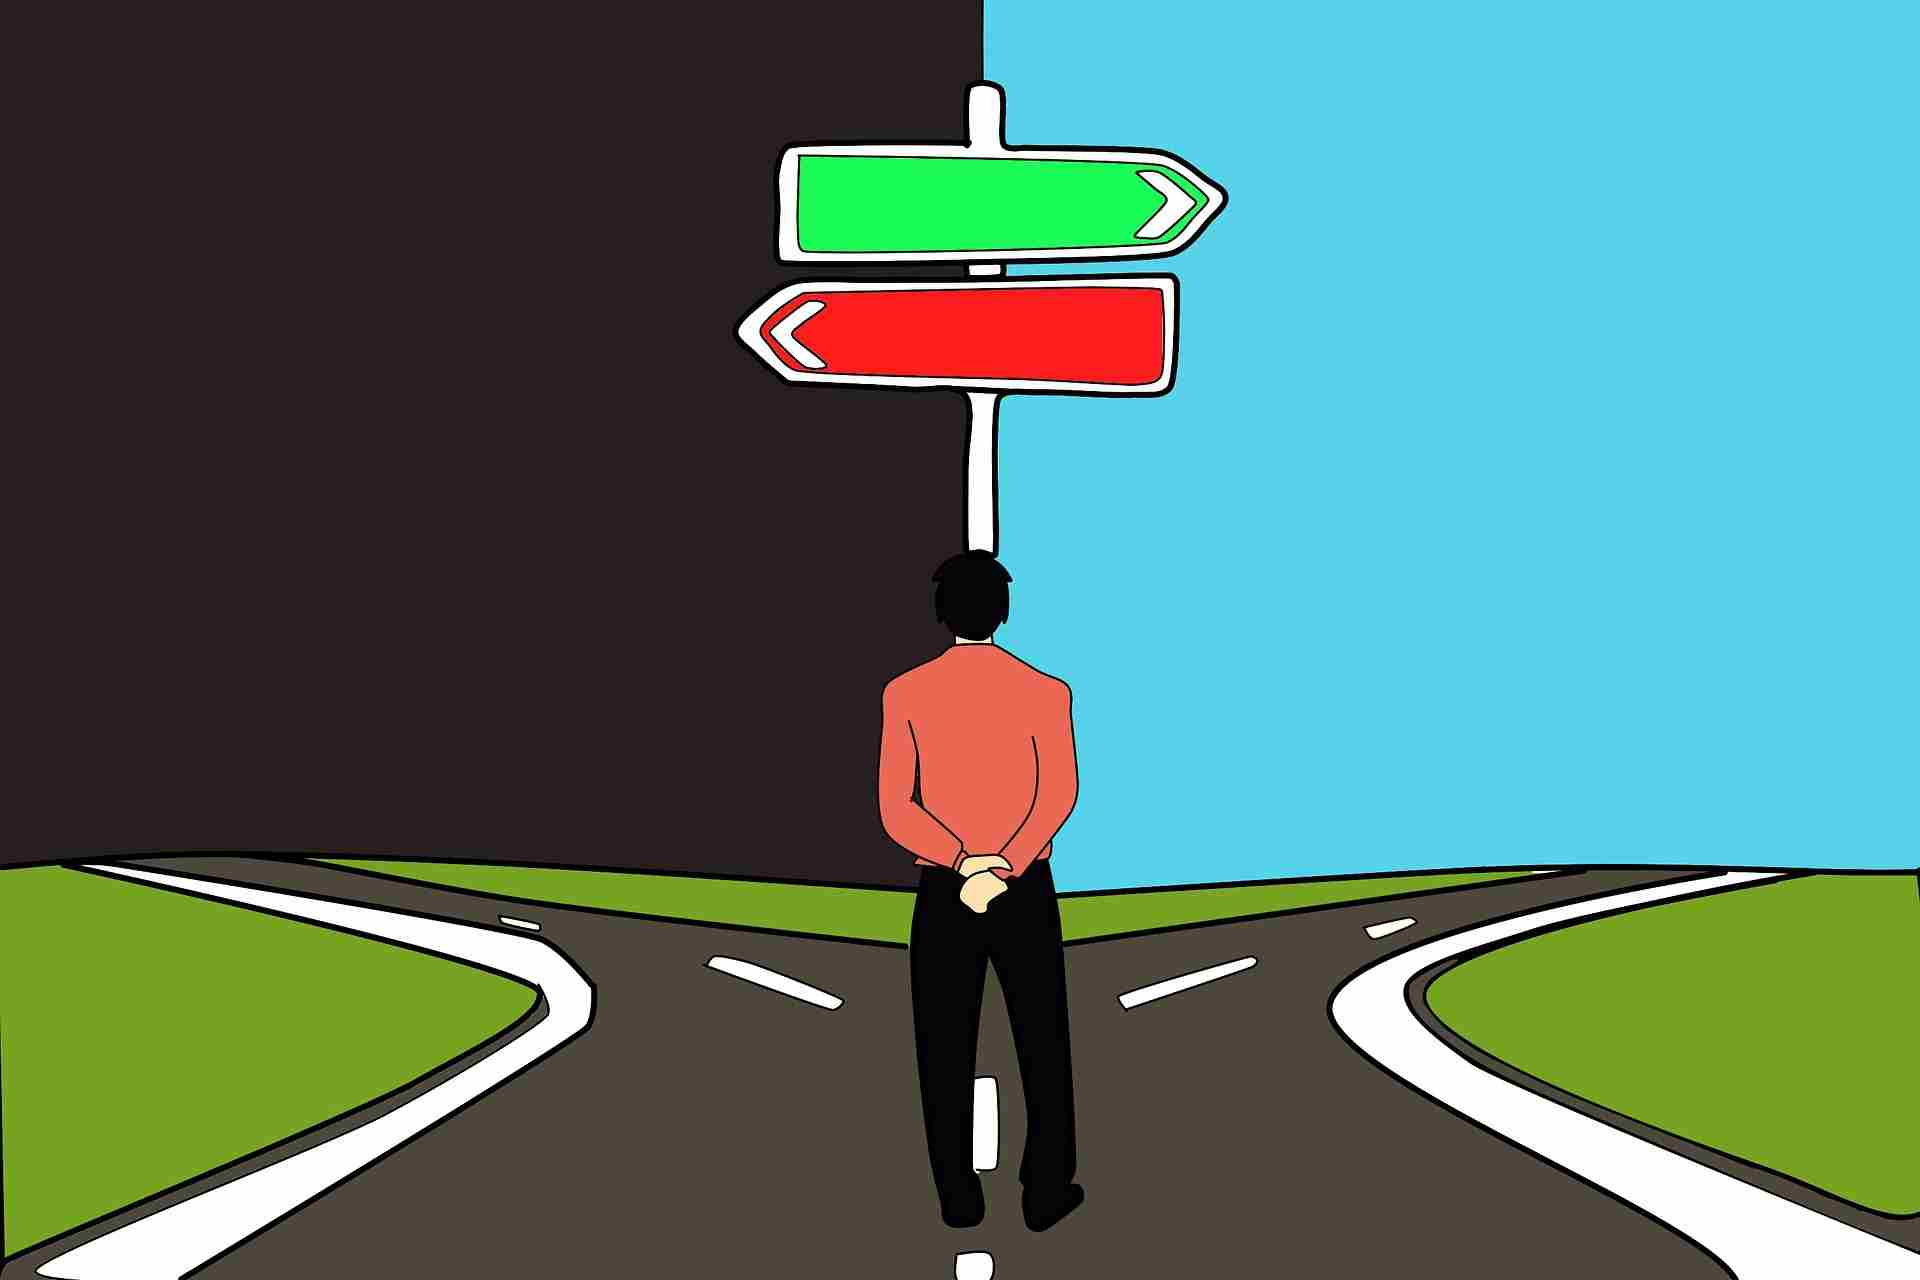
\includegraphics[width=0.5\textwidth,height=\textheight]{fig/decision-making.jpg}
\caption[\label{fig:decisionm} Decision-making]{\label{fig:decisionm} Decision-making\footnotemark{}}
\end{figure}
\footnotetext{Picture is taken from \url{https://pixabay.com/de/illustrations/entscheidung-auswahl-pfad-stra\%C3\%9Fe-1697537/}}

\hypertarget{types-of-decisions}{%
\section{Types of decisions}\label{types-of-decisions}}

Decision making is a process of investing time and effort to make a decision that will lead to (good) results. In the following, we discuss some types of decisions that can help to design an appropriate decision making process.

According to \citet[p.~9f]{Fitzgerald2002Decision} decisions can be roughly divided into two generic types:

\begin{itemize}
\tightlist
\item
  \textbf{routine decisions}: Decisions that must be made at regular intervals.
\item
  \textbf{non-routine}: Unique, random, non-recurring decision situations.
\end{itemize}

Another common method of dividing decisions into two categories is as follows:

\begin{itemize}
\tightlist
\item
  \textbf{Operative decisions}: This type of decision usually involves day-to-day business operations. There is a lot of overlap with the routine category here. Examples of this type of decision include setting production levels, deciding whether to hire or deciding whether to close a particular plant. When it comes to decisions in our daily lives, an example would be where, what, when, and what we eat for lunch.
\item
  \textbf{Strategic decisions}: This type of decision is usually about company policy and direction over a long period of time. Examples of strategic decisions include entering a new market, acquiring a competitor, or withdrawing from an industry. Renting an apartment near the university or commuting to our parents is an example of a strategic decision in our personal lives.
\end{itemize}

People often distinguish between decisions at work and private decisions. Private decisions affect fewer people on average, but usually the people involved are closer to you personally. However, both types of decisions involve the same things such as people (human resources), money (budgeting), buying and selling (marketing), how we do something (operations) or how we want to do it in the future (strategy and planning).

Some decisions are more important than others because the potential impact of a decision varies, i.e., the \textbf{scope of a decision}. For example, decisions can affect one person or millions, one pound/dollar or millions, one product/service or an entire market, one day or ten years, etc.

However, it is not entirely clear how to validate the scope. It depends heavily on the perspective of the decision-maker. For a small company, for example, an investment of 10,000 euros may be a big decision, while for a multinational cooperation it is a drop in the bucket. So the scope for decisions is relative, not absolute. It depends entirely on the context in which the decision is made and on the characteristics of the person(s) making it.

\hypertarget{three-conditions-of-decision-making}{%
\section{Three conditions of decision making}\label{three-conditions-of-decision-making}}

\begin{figure}
\centering
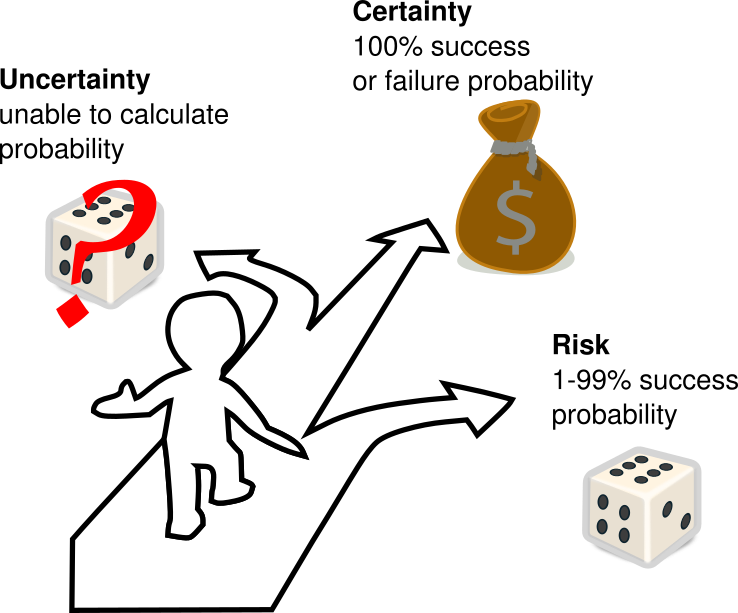
\includegraphics[width=0.5\textwidth,height=\textheight]{fig/risk-certainty-uncertainty.png}
\caption[\label{fig:3conditions} Conditions of decision making]{\label{fig:3conditions} Conditions of decision making\footnotemark{}}
\end{figure}
\footnotetext{Source: \citet{CEOpedia2021Rational}}

There are three general conditions (see \ref{fig:3conditions}) that determine the design of the optimal decision making process: certainty, risk and uncertainty.

\textbf{Certainty:}
A condition under which taking a decision involves reasonable degree of certainty about its result, what are the opportunities and what conditions accompany this decision.

\textbf{Risk:}
A condition under which taking a decision involves reasonable degree of certainty about its result, what are the opportunities and what conditions accompany this decision.

\textbf{Uncertainty:}
A condition in which decision maker does not know all the choices, as well as risks associated with each of them and possible consequences.

\hypertarget{decision-making-strategies}{%
\section{Decision making strategies}\label{decision-making-strategies}}

\begin{exercise}
\protect\hypertarget{exr:decisionstrategy}{}\label{exr:decisionstrategy}

Different schemes of a decision making process

\begin{enumerate}
\def\labelenumi{\alph{enumi})}
\item
  Google for \emph{``decision making strategies''} and look at the images that Google suggests you.
\item
  Read \citet{IET202312} and discuss the twelve decision making strategies. The article can be found \href{https://www.indeed.com/career-advice/career-development/decision-making-strategies?utm_campaign=earnedsocial\%3Acareerguide\%3Asharedirectshare\%3AUS\&utm_content=12\%20Decision-Making\%20Strategies\&utm_medium=social\&utm_source=directshare}{here}.
\item
  Compare these strategies to the scheme shown in figure \ref{fig:decision}.
\end{enumerate}

\begin{figure}
\centering
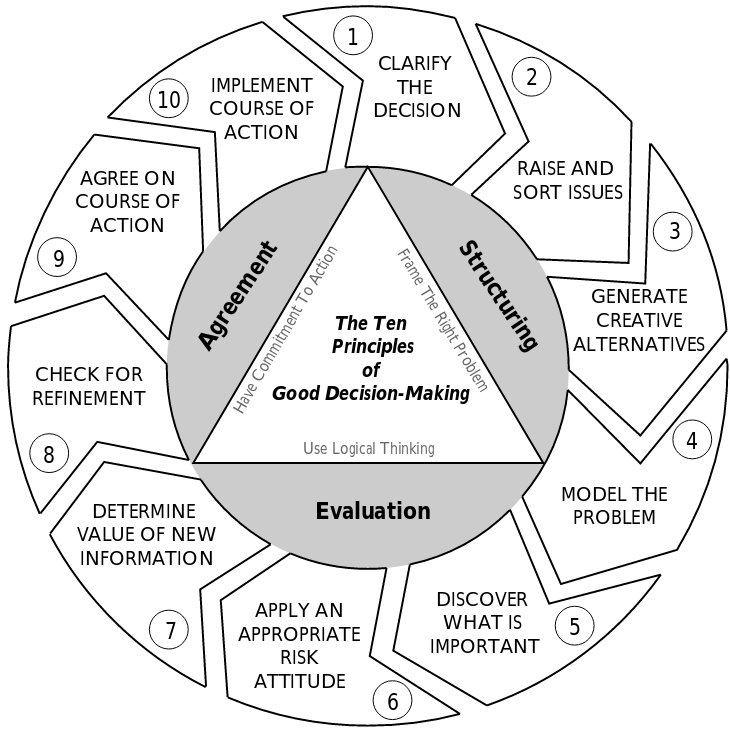
\includegraphics[width=0.5\textwidth,height=\textheight]{fig/tenprincipals_png.png}
\caption[\label{fig:decision} Decision-making]{\label{fig:decision} Decision-making\footnotemark{}}
\end{figure}
\footnotetext{Picture is taken from \url{https://pixabay.com/de/illustrations/entscheidung-auswahl-pfad-stra\%C3\%9Fe-1697537/}}

\begin{enumerate}
\def\labelenumi{\alph{enumi})}
\setcounter{enumi}{3}
\item
  Choose a problem of your choice and try to solve the problem using the two illustrations above by making a good decision.
\item
  Discuss in class whether the diagram or the strategies in \citet{IET202312} are helpful in making a wise decision or solving a problem.
\item
  Watch \url{https://youtu.be/pPIhAm_WGbQ} and answer the following questions: How is the nature of decisions discussed here? Does it contain a rational model of problem solving? Reflect on which ways to solve a problem and come to a decision, respectively, have been addressed.
\end{enumerate}

\end{exercise}

\begin{exercise}
\protect\hypertarget{exr:fisherman}{}\label{exr:fisherman}The businessman and the fisherman

A classic tale that exist in different version\^{}{[}This one stems from \href{https://thestorytellers.com/the-businessman-and-the-fisherman}{thestorytellers.com}. A famous version stems from Paulo Coelho\^{}{[}See \href{https://paulocoelhoblog.com/2015/09/04/the-fisherman-and-the-businessman/}{https://paulocoelhoblog.com} and it goes like this:

\begin{quote}
One day a fisherman was lying on a beautiful beach, with his fishing pole propped up in the sand and his solitary line cast out into the sparkling blue surf. He was enjoying the warmth of the afternoon sun and the prospect of catching a fish.

About that time, a businessman came walking down the beach, trying to relieve some of the stress of his workday. He noticed the fisherman sitting on the beach and decided to find out why this fisherman was fishing instead of working harder to make a living for himself and his family. ``You aren't going to catch many fish that way'', said the businessman to the fisherman.

``You should be working rather than lying on the beach!'' The fisherman looked up at the businessman, smiled and replied, ``And what will my reward be?'' ``Well, you can get bigger nets and catch more fish!'' was the businessman's answer. ``And then what will my reward be?'' asked the fisherman, still smiling. The businessman replied, ``You will make money and you'll be able to buy a boat, which will then result in larger catches of fish!'' ``And then what will my reward be?'''' asked the fisherman again.

The businessman was beginning to get a little irritated with the fisherman's questions. ``You can buy a bigger boat, and hire some people to work for you!'' he said. ``And then what will my reward be?'' repeated the fisherman. The businessman was getting angry. ``Don't you understand? You can build up a fleet of fishing boats, sail all over the world, and let all your employees catch fish for you!''

Once again the fisherman asked, ``And then what will my reward be?'' The businessman was red with rage and shouted at the fisherman, ``Don't you understand that you can become so rich that you will never have to work for your living again! You can spend all the rest of your days sitting on this beach, looking at the sunset. You won't have a care in the world!''

The fisherman, still smiling, looked up and said, ``And what do you think I'm doing right now?''
\end{quote}

Define the cost and benefits of both persons. Who do you think has a better life overall.
Who is acting rationally here? In other words, who is maximizing utility here? The fishermen or the businessmen? Both? None?
\end{exercise}

\hypertarget{the-rational-model}{%
\section{The rational model}\label{the-rational-model}}

Economists view the choices that people make as \emph{rational}. A rational choice is one that compares costs and benefits and achieves the greatest benefit over cost for the person making the choice. Whatever the benefits and the costs maybe, a decision maker have to consider all and make a decision. Of course, in reality it is often difficult if not impossinle to sum up benefits and costs as the nature of both may be totally different. To get rid of these problems economists use a theoretical concept that measures both in \emph{utility}. That is a general and abstract measure to model worth or value. Its usage has evolved significantly over time. The term was introduced initially as a measure of pleasure or happiness within the theory of utilitarianism. It represents the satisfaction or pleasure that people receive for consuming a bundle of goods and services, for example.

According to \citet{CEOpedia2021Rational} rational decision making is a style of decision making based on objective data and a formal process of analysis. It excludes acting based on subjective feelings and intuitive approach. The model assumes that deducting decisions with full information and all alternatives allows for the creation of cognitive skills that allow the evaluation of all possible options and then the selection of the best one.

It essentially consists of a logical sequence of steps. Here is an example taken from \citet[p.~13]{Fitzgerald2002Decision}:

\begin{enumerate}
\def\labelenumi{\arabic{enumi}.}
\item
  \textbf{Clearly identify the problem}. A \emph{problem} can be defined as a perceived gap between the current reality and the desired reality.
\item
  \textbf{Generate potential solutions}. For routine decisions, various alternatives can be identified relatively easily using predetermined decision rules, but non-routine decisions require a creative process to find new alternatives.
\item
  Using appropriate analytical approaches, select a solution from the available alternatives, preferably the one with the largest expected value. In decision theory, this is called \textbf{maximizing the expected utility of the outcomes}.
\item
  \textbf{Implement the solution}. Managers often undermine implementation by not ensuring that those responsible for implementation understand and accept what they need to do, and that they have the motivation and resources needed for successful implementation.
\item
  \textbf{Evaluate the effectiveness of the implemented decision}
\end{enumerate}

While these rational models may be helpful, they can also be criticized in a number of ways. In particular, it is a belief that managers actually optimize their decision behavior based on rationality because they consciously select and implement the best alternatives. This is a misconception because any rational optimization is based on a number of dubious assumptions. For example, (Fitzgerald, 2002, p.~13):

\begin{itemize}
\tightlist
\item
  it is hardly possible to know in advance all possible alternative solutions and to know in advance the specific outcomes that will result from each of them;
\item
  there is actually an optimal solution, and this solution is among the alternatives identified;
\item
  it is possible to accurately and numerically weight the various alternatives, the probabilities of their outcomes, and the relative desirability of these alternatives and outcomes;
\item
  the decision makers always act rationally and therefore the decision making is free of emotion, bias, and politics; and
\item
  business decisions are driven entirely by the desire to maximize profits.
\end{itemize}

The \textbf{rational model can be considered normative} because it prescribes a strict logical sequence of steps to be followed in any decision-making situation. The rational models are based on the assumption that human behavior is logical and therefore predictable under certain circumstances. This is not necessarily what actually happens in the real world. Consider, for example, the findings in the field of behavioral economics, which clearly show that homo economicus is a (useful) concept that is weak in several aspects.

\hypertarget{bounded-rationality}{%
\section{Bounded rationality}\label{bounded-rationality}}

\begin{figure}
\centering
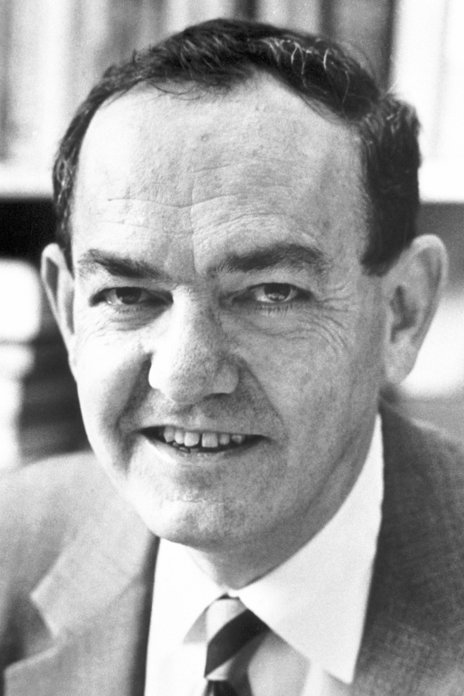
\includegraphics[width=0.2\textwidth,height=\textheight]{fig/herbert-simon.jpg}
\caption[\label{fig:simon} Herbert A. Simon]{\label{fig:simon} Herbert A. Simon\footnotemark{}}
\end{figure}
\footnotetext{Picture is taken from \href{https://www.nobelprize.org/images/simon-13300-portrait-mini-2x.jpg}{Nobel Foundation archive}}

Herbert A. Simon (1916-2001) shown in figure \ref{fig:simon} received the Nobel Memorial Prize in Economic Sciences in 1978 and the Turing Award\footnote{The Turing Award is an annual prize given by the Association for Computing Machinery (ACM) for contributions of lasting and major technical importance to the computer field. It is generally recognized as the highest distinction in computer science and is known as or often referred to as `Nobel Prize of Computing'.} in 1975. According to \citet{NobelPrize.org2021Herbert}, he

\begin{quote}
``combined different scientific disciplines and considered new factors in economic theories. Established economic theories held that enterprises and entrepreneurs all acted in completely rational ways, with the maximization of their own profit as their only goal. In contrast, Simon held that when making choices all people deviate from the strictly rational, and described companies as adaptable systems, with physical, personal, and social components. Through these perspectives, he was able to write about decision-making processes in modern society in an entirely new way''.
\end{quote}

In particular, he proposed \textbf{bounded rationality} as an alternative basis for the mathematical and neoclassical economic modelling of decision-making, as used in economics, political science, and related disciplines.

\begin{figure}
\centering
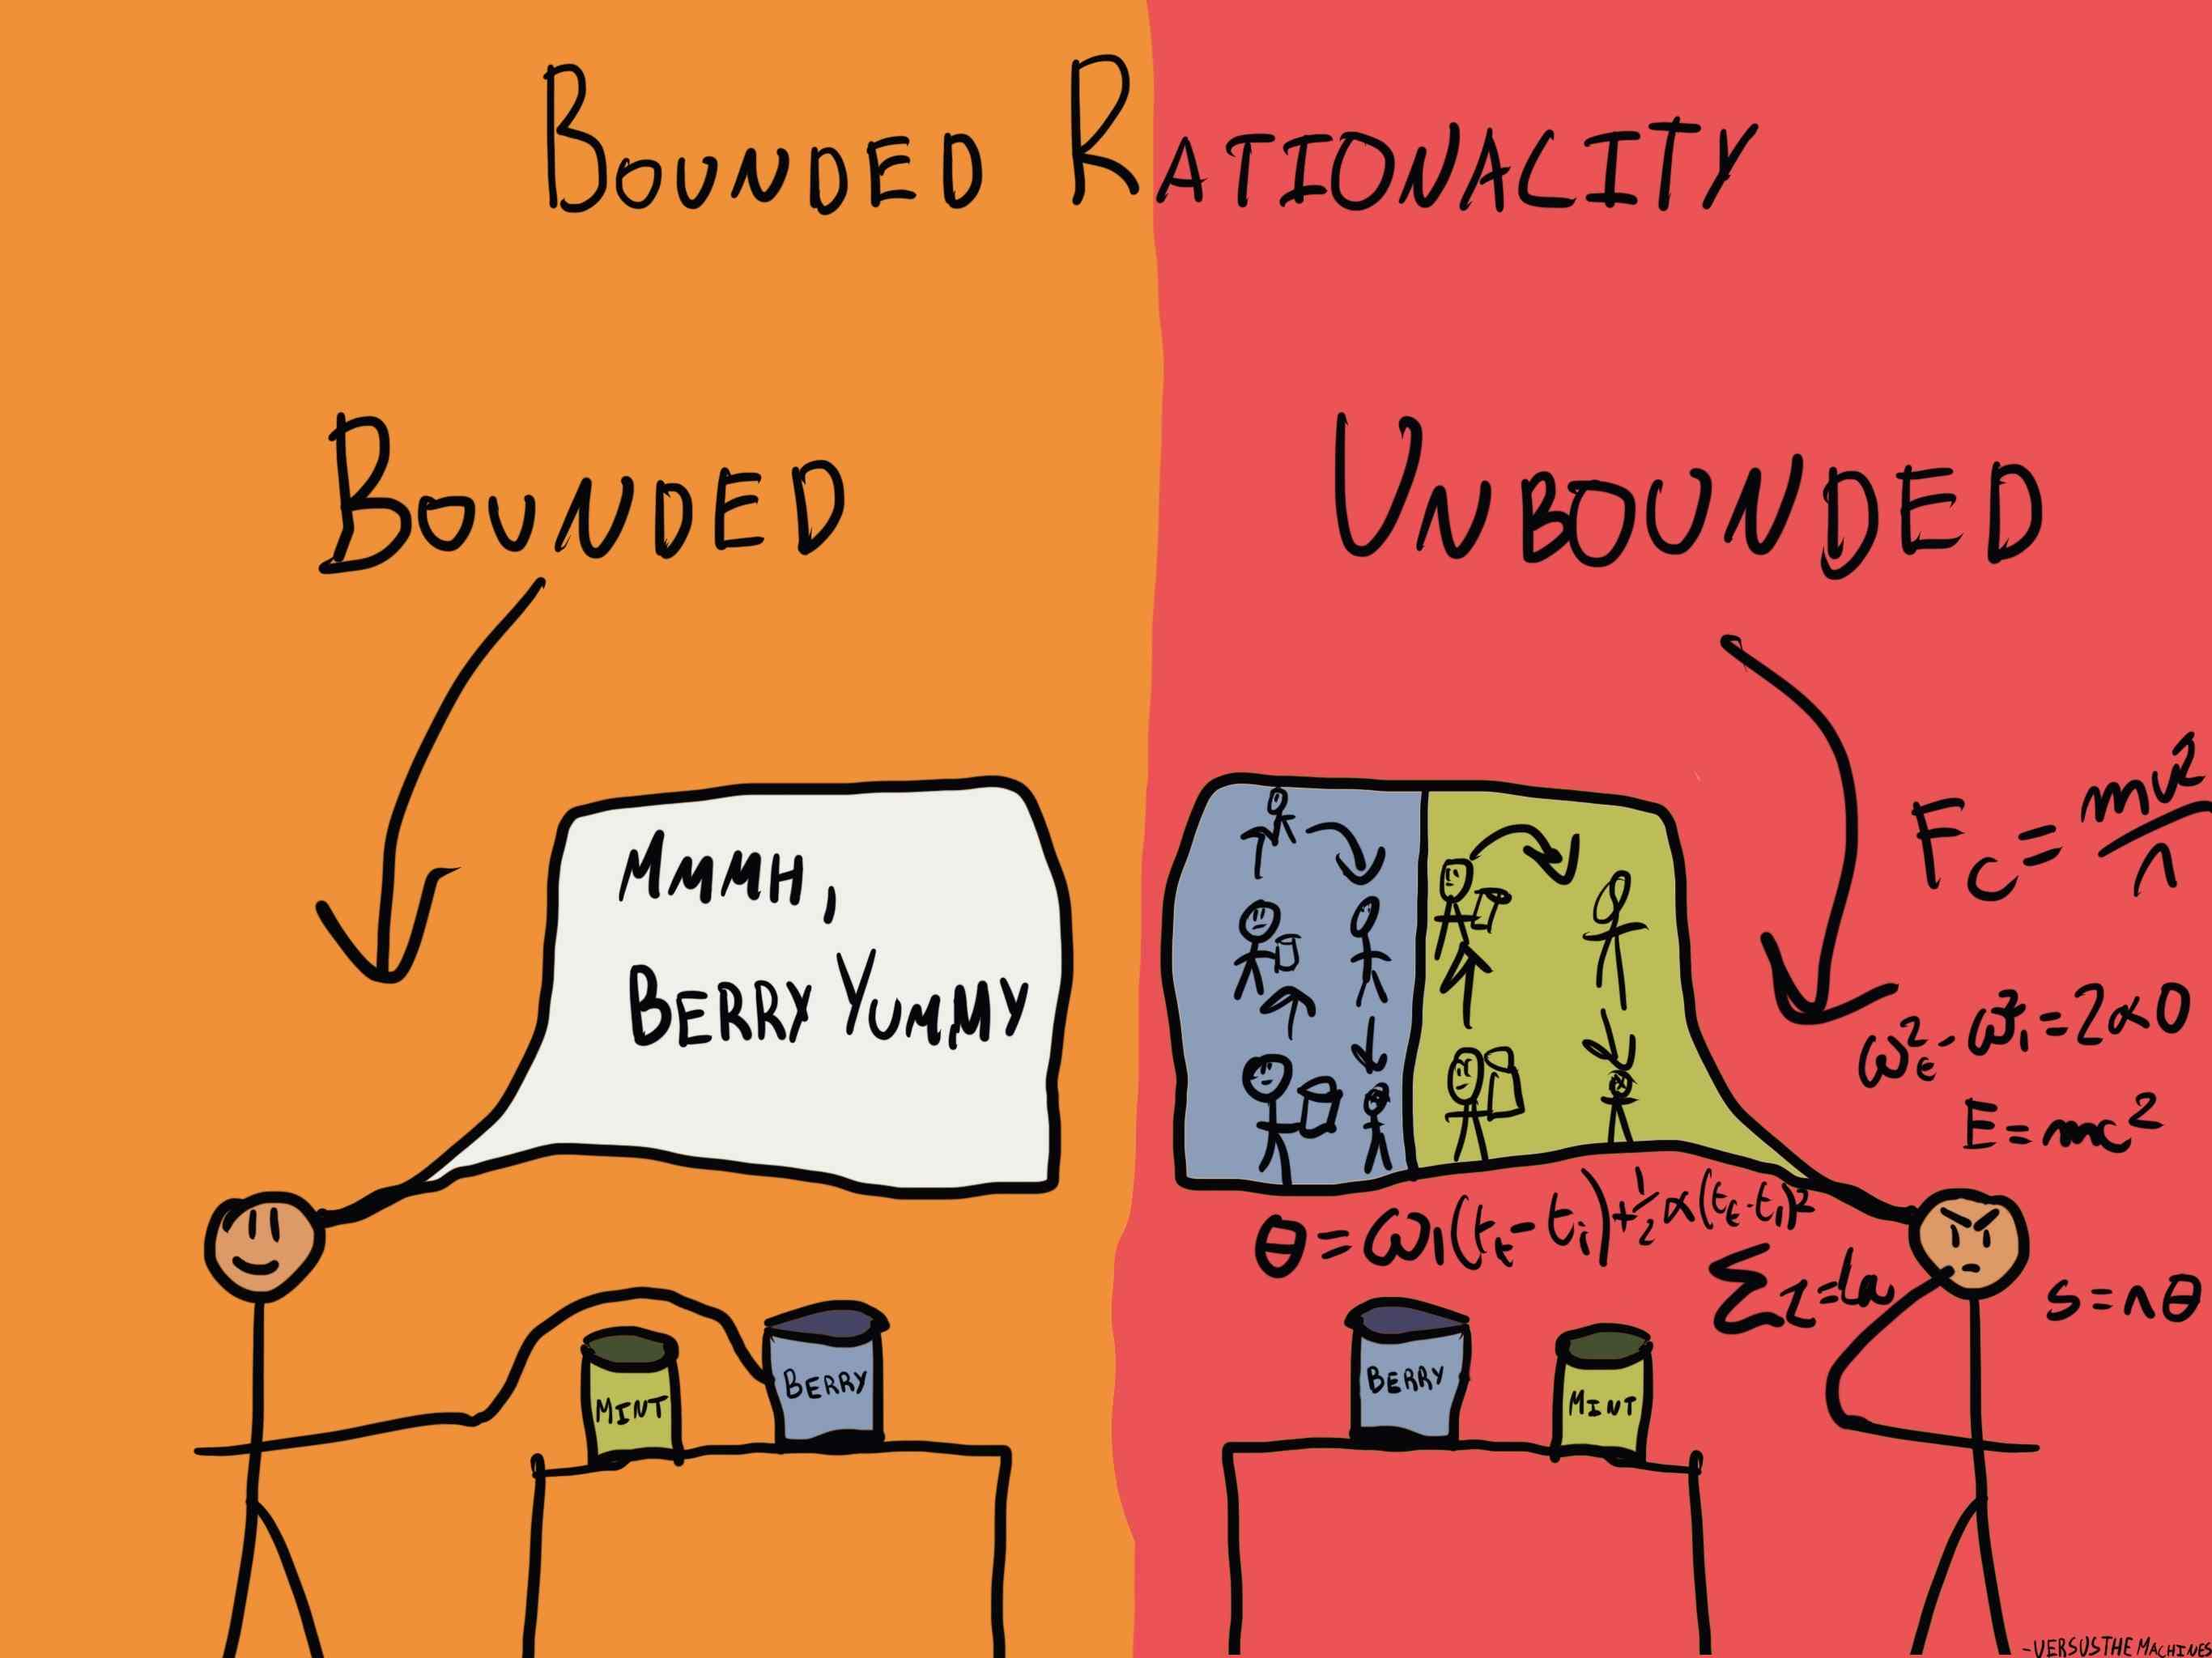
\includegraphics[width=0.5\textwidth,height=\textheight]{fig/bounded-rationality.jpg}
\caption[\label{fig:boundedrationality} Bounded rationality]{\label{fig:boundedrationality} Bounded rationality\footnotemark{}}
\end{figure}
\footnotetext{Picture is taken from \url{https://thedecisionlab.com/wp-content/uploads/2019/08/Bounded-Rationality.jpg}}

Bounded rationality proposes that decision making is constrained by managers' ability to process information, i.e., the rationally is \emph{bounded} (see figure \ref{fig:boundedrationality}). Managers use shortcuts and rules of thumb which are based on their prior experience with similar problems and scenarios. Given the constraints of managers in their position, they do not actually \emph{optimize} their choice given the available information. It is more like finding a \emph{satisfactory} solution, not necessarily the \emph{best} or the \emph{optimal} solution.

\begin{exercise}
\protect\hypertarget{exr:opti-sati}{}\label{exr:opti-sati}

Optimal vs.~satisfactory solution

Using the images \ref{fig:picA} to \ref{fig:picD}, explain the idea of bounded rationality in the context of decision making.

\begin{figure}
\centering

\includegraphics[width=0.45\textwidth,height=\textheight]{fig/seeking.jpg}
\caption{\label{fig:picA} Picture A}
\end{figure}

\begin{figure}
\centering

\includegraphics[width=0.45\textwidth,height=\textheight]{fig/thumb.jpg}
\caption{\label{fig:picB} Picture B}
\end{figure}

\begin{figure}
\centering
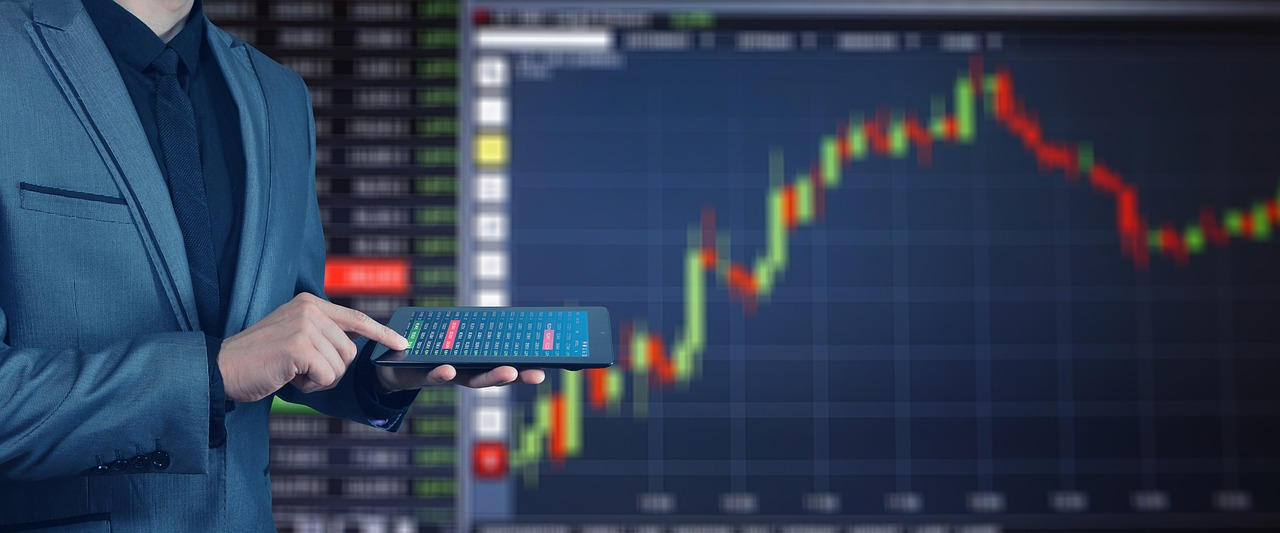
\includegraphics[width=0.45\textwidth,height=\textheight]{fig/stock.jpg}
\caption{\label{fig:picC} Picture C}
\end{figure}

\begin{figure}
\centering
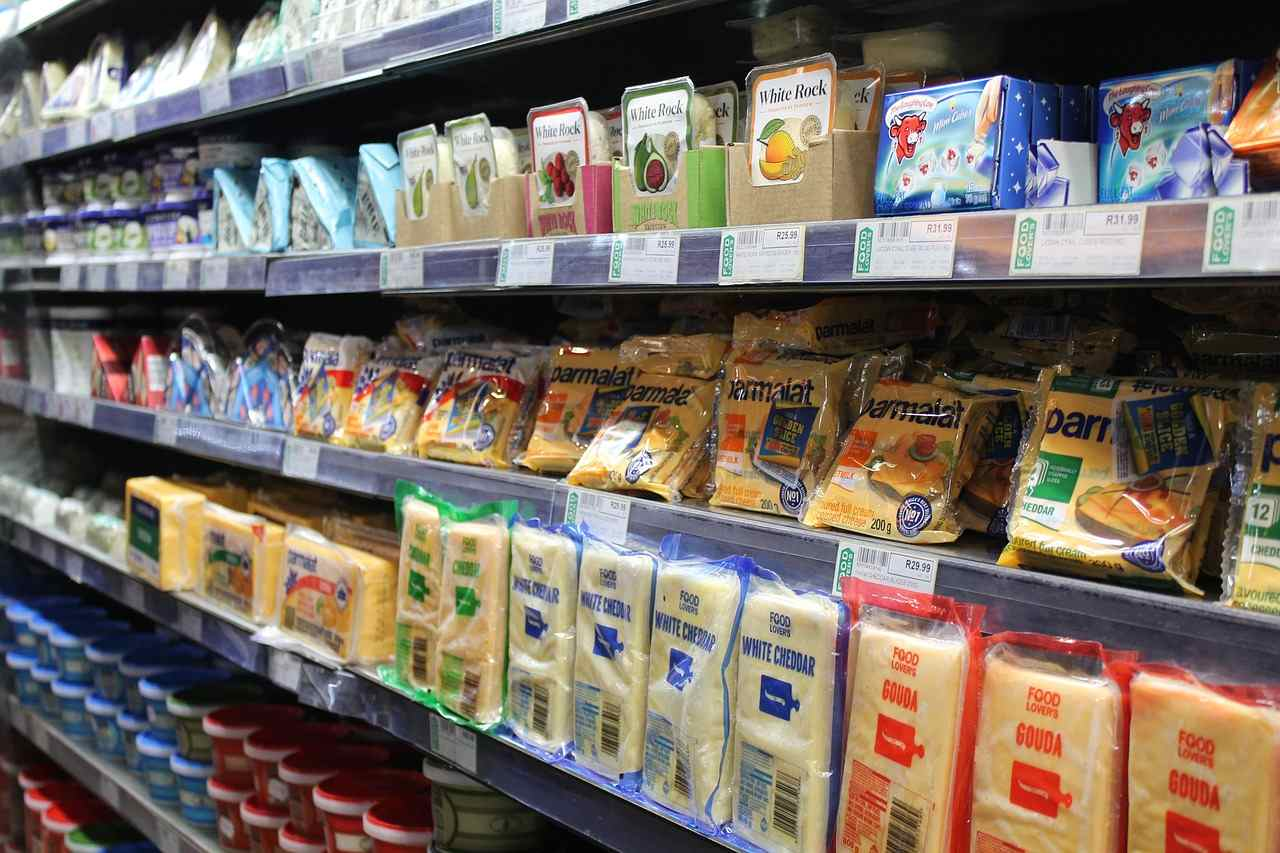
\includegraphics[width=0.45\textwidth,height=\textheight]{fig/supermarket.jpg}
\caption{\label{fig:picD} Picture D}
\end{figure}

Please find solution to the exercise \protect\hyperlink{sol:opti-sati}{in the appendix.}

\begin{center}\rule{0.5\linewidth}{0.5pt}\end{center}

\end{exercise}

\begin{exercise}
\protect\hypertarget{exr:irrational}{}\label{exr:irrational}

Are we irrational?

Discuss the following statement:

\begin{quote}
Since the rationality of individuals is bounded and it is obvious that individuals do not make optimal decisions, we can say that individuals act irrationally.
\end{quote}

\end{exercise}

\hypertarget{homo-economicus}{%
\section{Homo economicus}\label{homo-economicus}}

The so-called \emph{homo economicus} is often modeled by the assumption of perfect rationality. Actors are assumed to always act in a way that maximizes their utility (as consumers) and profit (as producers), and to this end they are capable of arbitrarily complex reasoning. That is, it is assumed that they are always capable of thinking through all possible outcomes and choosing the course of action that leads to the best possible outcome.

Of course, the assumption of \emph{homo economicus} is heroic, and I doubt that any serious economist has ever assumed that this assumption can be found one-to-one in reality. However, it is an assumption that helps to make predictions and explain the behavior of people and societies to some extent. I mean, what would happen if microeconomics went to the other extreme assuming irrationally acting individuals. The result would be, more or less, that we would not be able to make predictions and the future would be a random walk.

Nevertheless, economists and anyone who wants to make, apply, or think about economic theories should be aware of all the pitfalls that arise in our decision making and know that our ability to act rationally is limited. In real life, we often use heuristics to solve problems and make decisions.

A \textbf{heuristic} is any approach to solving a problem that uses a practical method that is not guaranteed to be optimal, perfect, or rational. However, a heuristic should--at best--be sufficient to achieve an immediate, short-term goal or approximation. Overall, people use heuristics because they either cannot act completely rationally or want to act rationally but do not have the time it would take to compute the perfect solution. Moreover, the effort is probably not worth it or simply not possible given the time constraints under which the problem must be solved.
A heuristic is a mental shortcut or rule of thumb to make decisions and solve problems quickly and efficiently. It helps individuals to arrive at a solution without extensive analysis or evaluation of all available information. Heuristics are usefull when time, resources, or information are limited.

While heuristics can be helpful in many situations, they can also lead to errors and biases, particularly when they are overused or misapplied. We will discuss some of these biases in section \ref{cognitive-biases} in greater detail.

\hypertarget{decision-trees}{%
\section{Decision trees}\label{decision-trees}}

When we decide under certain conditions, decision trees can be a helpful tool, as explained in \citep{Finne1998three}. If you want to know more about the use of decision trees I recommend reading \citet[ch.~4]{Bonanno2017Decision}.

\hypertarget{payoff-table}{%
\section{Payoff table}\label{payoff-table}}

A payoff table, also known as a decision matrix, can be a helpful tool for decision making, as shown in the table below. It presents the available alternatives denoted by \(A_i\), along with the possible future states of nature or goals denoted by \(N_j\).

The payoff or outcome depends on both the chosen alternative and the future state of nature that occurs. For instance, if alternative \(A_i\) is chosen and state of nature \(N_j\) occurs, the resulting payoff is \(O_{ij}\). Our goal is to choose the alternative \(A_i\) that yields the most favorable outcome \(O_{ij}\).

\begin{longtable}[]{@{}
  >{\raggedright\arraybackslash}p{(\columnwidth - 12\tabcolsep) * \real{0.3143}}
  >{\raggedright\arraybackslash}p{(\columnwidth - 12\tabcolsep) * \real{0.1571}}
  >{\raggedright\arraybackslash}p{(\columnwidth - 12\tabcolsep) * \real{0.1000}}
  >{\raggedright\arraybackslash}p{(\columnwidth - 12\tabcolsep) * \real{0.1143}}
  >{\raggedright\arraybackslash}p{(\columnwidth - 12\tabcolsep) * \real{0.1143}}
  >{\raggedright\arraybackslash}p{(\columnwidth - 12\tabcolsep) * \real{0.1143}}
  >{\raggedright\arraybackslash}p{(\columnwidth - 12\tabcolsep) * \real{0.0857}}@{}}
\caption{Payoff matrix}\tabularnewline
\toprule\noalign{}
\endfirsthead
\endhead
\bottomrule\noalign{}
\endlastfoot
State of nature (\(N_j\)) & \(N_1\) & \(N_2\) & \(\cdots\) & \(N_j\) & \(\cdots\) & \(N_n\) \\
Probability (p) & \(p_1\) & \(p_2\) & \(\cdots\) & \(p_j\) & \(\cdots\) & \(p_n\) \\
Alternative (\(A_i\)) & & & & & & \\
\(A_1\) & \(O_{11}\) & \(O_{12}\) & \(\cdots\) & \(O_{1j}\) & \(\cdots\) & \(O_{1n}\) \\
\(A_2\) & \(O_{21}\) & \(O_{22}\) & \(\cdots\) & \(O_{2j}\) & \(\cdots\) & \(O_{2n}\) \\
\(\cdots\) & \(\cdots\) & \(\cdots\) & \(\cdots\) & \(\cdots\) & \(\cdots\) & \(\cdots\) \\
\(A_i\) & \(O_{i1}\) & \(O_{i2}\) & \(\cdots\) & \(O_{ij}\) & \(\cdots\) & \(O_{in}\) \\
\(\cdots\) & \(\cdots\) & \(\cdots\) & \(\cdots\) & \(\cdots\) & \(\cdots\) & \(\cdots\) \\
\(A_m\) & \(O_{m1}\) & \(O_{m2}\) & \(\cdots\) & \(O_{mj}\) & \(\cdots\) & \(O_{mn}\) \\
\end{longtable}

If we assume that all objectives are independent from each other and that we are certain about the state of nature, the decision is rather trivial: just go for the alternative with the best outcome for each state of nature. However, most real-world scenarios are not that simple because most states of nature are more complex and needs further to be considered.

\hypertarget{review}{%
\section{Review}\label{review}}

\begin{itemize}
\tightlist
\item
  Decision analysis is about using information in order to come to a decision.
\item
  A structured and rational process can help improve the chances of receiving good decision outcomes.
\item
  As decision problems are often (too) complex to fully capture or solve rationally. Thus, a good decision analysis should try to use the available information and the existing understanding of the problem as transparent, consistent, and logical as possible.
\item
  A complex decision problem should be simplified and hence decomposed into its basic and most important components.
\item
  There are hundred of different \emph{schemes} or \emph{strategies} how to make decisions in certain circumstances. Many heuristics exist how to think, behave, and calculate to come to a wise decision.
\item
  Mostly decisions are based on subjective expectations. These expectations are difficult to validate.
\item
  Articulating exact expectation and preferences is a difficult task and the information that stems from these articulation is full of biases. Decision analytic tools need to take that into consideration.
\end{itemize}

\begin{exercise}
\protect\hypertarget{exr:lisapregnant}{}\label{exr:lisapregnant}

Lisa is pregnant

The following question stems from a study carried out by \citet{Kahneman1972Subjective}: Lisa is thirty-three and is pregnant for the first time. She is worried about birth defects such as Down syndrome. Her doctor tells her that she need not worry too much because there is only a 1 in 1,000 chance that a woman of her age will have a baby with Down syndrome. Nevertheless, Lisa remains anxious about this possibility and decides to obtain a test, known as the Triple Screen, that can detect Down syndrome. The test is moderately accurate: When a baby has Down syndrome, the test delivers a positive result 86 percent of the time. There is, however, a small `false positive' rate: 5 percent of babies produce a positive result despite not having Down syndrome. Lisa takes the Triple Screen and obtains a positive result for Down syndrome.

Given this test result, what are the chances that her baby has Down syndrome?

\begin{enumerate}
\def\labelenumi{\alph{enumi})}
\tightlist
\item
  0-20 percent chance
\item
  21-40 percent chance
\item
  41-60 percent chance
\item
  61-80 percent chance
\item
  81-100 percent chance
\end{enumerate}

Think about the question and put your answer here:

\url{https://pingo.coactum.de/} Code: 666528

Please find solution to the exercise \protect\hyperlink{sol:lisapregnant}{in the appendix.}

\begin{center}\rule{0.5\linewidth}{0.5pt}\end{center}

\end{exercise}

\hypertarget{decision-making-theory}{%
\chapter{Decision making theory}\label{decision-making-theory}}

\hypertarget{decision-making-under-certainty}{%
\section{Decision making under certainty}\label{decision-making-under-certainty}}

\begin{center}\rule{0.5\linewidth}{0.5pt}\end{center}

After successful completion of the module, students are able to:

\begin{itemize}
\tightlist
\item
  Distinguish different theories of decision making.
\item
  Calculate the optimal decision under certainty, uncertainty, and under risk.
\item
  Describe and use various criteria of decision making.
\item
  Simplify complex decision making situations and use formal approaches of decision making to guide the decision making behavior of managers.
\item
  Avoid common mistakes when applying heuristics in decision making.
\item
  Use investment calculus to make good financial decisions.
\end{itemize}

\begin{center}\rule{0.5\linewidth}{0.5pt}\end{center}

Decision making under certainty means that we assume that we are certain about the future state of nature, i.e., we have complete information about the alternative actions and their consequences. Making decisions under certainty may seem like a trivial exercise. However, many problems are so complex that sophisticated mathematical techniques are sometimes needed to find the best solution.

\hypertarget{decision-making-with-complex-state-of-natures}{%
\subsection{Decision making with complex state of natures}\label{decision-making-with-complex-state-of-natures}}

Suppose you have to decide between four different restaurants where you want to go out to eat (\(a_1\), \(a_2\), \(a_3\), \(a_4\)). The restaurants have different characteristics such as the quality of the food k1, the quality of the music played \(k_2\), the price \(k_3\), the quality of the service \(k_4\), and the environment \(k_5\). The corresponding payoff table is given below. High numbers represent good quality. In other words, \(a_i\) refer to competing alternatives where to eat for dinner, and \(k_i\) are certain characteristics of the respective restaurant, and the numbers given in the table indicate the output.

\begin{longtable}[]{@{}cccccc@{}}
\caption{Weighting scheme}\tabularnewline
\toprule\noalign{}
& \(k_1\) & \(k_2\) & \(k_3\) & \(k_4\) & \(k_5\) \\
\midrule\noalign{}
\endfirsthead
\toprule\noalign{}
& \(k_1\) & \(k_2\) & \(k_3\) & \(k_4\) & \(k_5\) \\
\midrule\noalign{}
\endhead
\bottomrule\noalign{}
\endlastfoot
\(a_1\) & 3 & 0 & 7 & 1 & 4 \\
\(a_2\) & 4 & 1 & 4 & 2 & 1 \\
\(a_3\) & 4 & 0 & 3 & 2 & 1 \\
\(a_4\) & 5 & 1 & 2 & 3 & 1 \\
\end{longtable}

\hypertarget{domination}{%
\subsection*{Domination}\label{domination}}

Some alternative can be excluded because they are \textbf{dominated} by other alternatives. In the scheme above you can see that alternative 2 is always superior to alternative 3, i.e., alternative 3 is dominated by alternative 2. Thus, it does not make sense to think about alternative 3:

\begin{longtable}[]{@{}cccccc@{}}
\caption{Alternative 3 is dominated by alternative 2}\tabularnewline
\toprule\noalign{}
& \(k_1\) & \(k_2\) & \(k_3\) & \(k_4\) & \(k_5\) \\
\midrule\noalign{}
\endfirsthead
\toprule\noalign{}
& \(k_1\) & \(k_2\) & \(k_3\) & \(k_4\) & \(k_5\) \\
\midrule\noalign{}
\endhead
\bottomrule\noalign{}
\endlastfoot
\(a_1\) & 3 & 0 & 7 & 1 & 4 \\
\(a_2\) & 4 & 1 & 4 & 2 & 1 \\
\(a_3\) & \st{4} & \st{0} & \st{3} & \st{2} & \st{1} \\
\(a_4\) & 5 & 1 & 2 & 3 & 1 \\
\end{longtable}

\hypertarget{weighting}{%
\subsection*{Weighting}\label{weighting}}

As the objectives \(k_j\) of the scheme above do not represent different states of nature but represent characteristics and its corresponding utility (whatever that number may mean in particular) of one particular characteristics if we choose a respective alternative. For example, think of that you can choose one out of four restaurants, \(a_1,\dots,a_4\), in order to eat a five-course menu, \(k_1,\dots,k_5\), and the outcome represents your utility of each course, \(j\), for each restaurant, \(i\). We already know from the domination principle that restaurant \(a_3\) is a bad choice.

Suppose you have a preference for the first three courses. Specifically, suppose that your preference scheme is as follows:

\[
g_1 : g_2 : g_3 : g_4 : g_5 = 3 : 4 : 3 : 1 : 1
\]

This means, for example, that you value the second food course four times more than the last course.

\[
w_1=3/12; w_2=4/12; w_3=3/12; w_4 = w_5 =1/12.
\]

In order to find a decision criteria you can calculate the aggregated expected utility as follows:

\[
\Phi(a_i)=\sum_{p=1}^{r}w_p\cdot u_{ip} \rightarrow max
\]

The results are as follows:

\begin{longtable}[]{@{}ccccccc@{}}
\toprule\noalign{}
& \(k_1\) & \(k_2\) & \(k_3\) & \(k_4\) & \(k_5\) & \(\Phi(a_i)\) \\
\midrule\noalign{}
\endhead
\bottomrule\noalign{}
\endlastfoot
\(a_1\) & 3 & 0 & 7 & 1 & 4 & 35//12 \\
\(a_2\) & 4 & 1 & 4 & 2 & 1 & 31//12 \\
\(a_3\) & 4 & 0 & 3 & 2 & 1 & 24//12 \\
\(a_4\) & 5 & 1 & 2 & 3 & 1 & 29//12 \\
\end{longtable}

Thus, \(a_1\succ a_2 \succ a_4 \succ a_3\), i.e., you prefer alternative \(a_1\).

\hypertarget{preferences-and-decision-criteria}{%
\subsection*{Preferences and decision criteria}\label{preferences-and-decision-criteria}}

Maybe not all courses play the same role for you so you can take your decision based on your preference scheme. For example, assume some courses are more important to you than others such as \(k_1 \succ k_3 \succ k_2 \succ k_4 \succ k_5\). Now, if you decide based on your most important course you should choose restaurant 4 because this gives you the highest utility in that dish. If you further assume that you are not that hungry and you only like to have two dishes, then you should probably better go for restaurant 1 because the aggregated utility in the two preferred courses is 10 utility units and restaurants 2, 3 and 4 can only offer 8, 7 and 7 utility units in your two preferred courses.

\hypertarget{kuxf6rths-maximin-rule}{%
\subsection*{Körth's Maximin-Rule}\label{kuxf6rths-maximin-rule}}

According to this rule, we compare alternatives by the worst possible outcome under each alternative, and we should choose the one which maximizes the utility of the worst outcome. More concrete, the procedure consists of 4 steps:

\begin{enumerate}
\def\labelenumi{\arabic{enumi}.}
\tightlist
\item
  Calculate the utility maximum for each column \(j\) of the payoff matrix: \[\overline{O}_j=\max_{i=1,\dots,m}{O_{ij}}\qquad \forall j.\]
\item
  Calculate for each cell the relative utility, \[\frac{O_{ij}}{\overline{O}_j}.\]
\item
  Calculate for each row \(i\) the minimum: \[\Phi(a_i)=\min_{j=1,\dots,p}\left(\frac{O_{ij}}{\overline{O}_j}\right) \qquad \forall i.\]
\item
  Set preferences by maximizing \(\Phi(a_i)\).
\end{enumerate}

\hypertarget{linear-programming}{%
\subsection{Linear programming}\label{linear-programming}}

Linear Programming is a common technique for decision making under certainty. It allows to express a desired benefit (such as profit) as a mathematical function of several variables. The solution is the set of values for the independent variables (decision variables) that serves to maximize the benefit or to minimize the negative outcome under consideration of certain limits, a.k.a. constraints. The method usually follows a four step procedure:

\begin{enumerate}
\def\labelenumi{\arabic{enumi}.}
\tightlist
\item
  state the problem;
\item
  state the decision variables;
\item
  set up an objective function;
\item
  clarify the constraints.
\end{enumerate}

\textbf{Example:}
Consider a factory producing two products, product X and product Y. The problem is this: If
you can realize \$10.00 profit per unit of product X and \$14.00 per unit of product Y, what is the production level of x units of product X and y units of product Y that maximizes the profit P each day? Your production, and therefore your profit, is subject to resource limitations, or constraints. Assume in this example that you employ five workers---three machinists and two assemblers---and that each works only 40 hours a week.\footnote{The example is taken from \citet[p.~134f]{Morse2014Managing}.}

\begin{itemize}
\tightlist
\item
  Product X requires three hours of machining and one hour of assembly per unit.
\item
  Product Y requires two hours of machining and two hours of assembly per unit.
\end{itemize}

\begin{enumerate}
\def\labelenumi{\arabic{enumi}.}
\tightlist
\item
  \emph{State the problem:} How many of product X and product Y to produce to maximize profit?
\item
  \emph{Decision variables:} Suppose x denotes the number of product X to produce per day and y denotes number of product Y to produce per day
\item
  \emph{Objective function:} Maximize \[P = 10x + 14y\]
\item
  \emph{Constraints:}
\end{enumerate}

\begin{itemize}
\tightlist
\item
  machine time=120h
\item
  assembling time=80h
\item
  hours needed for production of one good:
\end{itemize}

\emph{machine time:} \(x\rightarrow 3h\) and \(y \rightarrow 2h\)

\emph{assembling time:} \(x\rightarrow 1h\) and \(y \rightarrow 2h\)

Thus, we get:
\[3x + 2y \leq 120 \quad \Leftrightarrow y\leq 60-\frac{3}{2}x \quad \text{(hours of machining time)}\]
\[x + 2y \leq 80 \quad \Leftrightarrow y \leq 40-\frac{1}{2}x \quad \text{(hours of assembly time)}\]
Since there are only two products, these limitations can be shown on a two-dimensional graph (\ref{fig:lpe2}). Since all relationships are linear, the solution to our problem will fall at one of the corners.

\begin{figure}
\centering
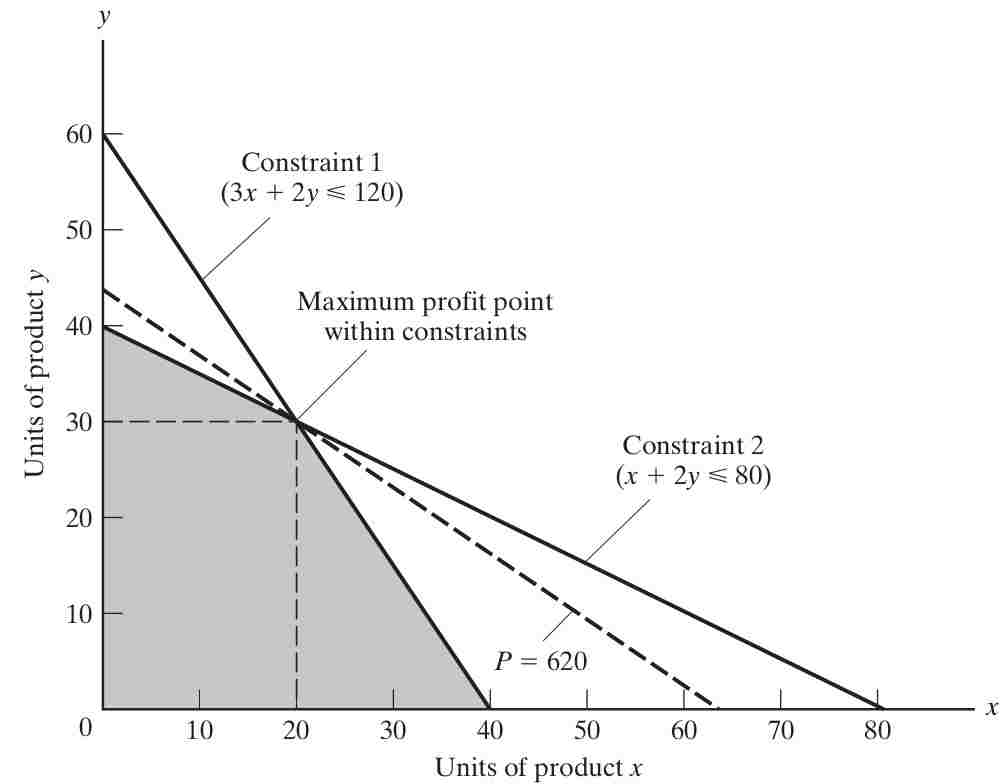
\includegraphics[width=0.75\textwidth,height=\textheight]{fig/lpe2.jpg}
\caption{\label{fig:lpe2} Linear program example: constraints and solution}
\end{figure}

To draw the isoprofit function in a plot with the good \(y\) on the y-axis and good \(x\) on the x-axis, we can re-arrange the objective function to get \[y=\frac{1}{14}P-\frac{10}{14}x\]
To illustrate the function let us consider some arbitrarily chosen levels of profit in \autoref{fig:lpe}:

\begin{itemize}
\tightlist
\item
  \$350 by selling 35 units of X or 25 units of Y
\item
  \$700 by selling 70 units of X or 50 units of Y
\item
  \$620 by selling 62 units of X or 44.3 units of Y.
\end{itemize}

\begin{figure}
\centering
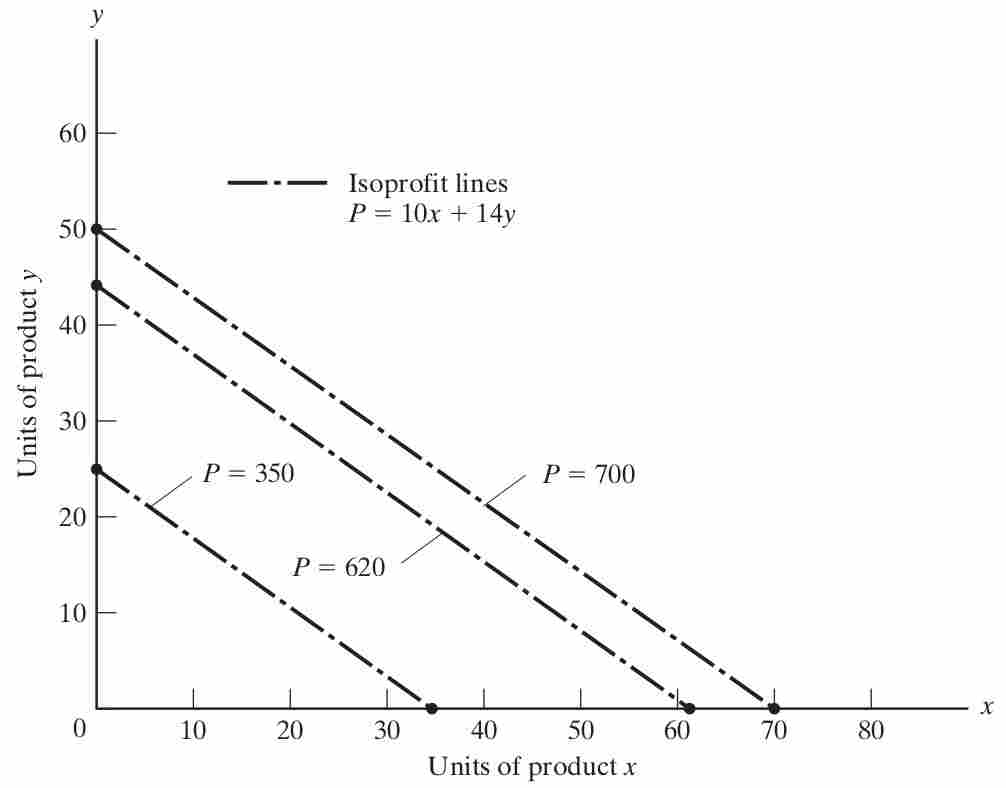
\includegraphics[width=0.75\textwidth,height=\textheight]{fig/lpe.jpg}
\caption{\label{fig:lpe} Linear program example: isoprofit lines}
\end{figure}

To find the solution, begin at some feasible solution (satisfying the given constraints) such as \((x,y) = (0,0)\), and proceed in the direction of \emph{steepest ascent} of the profit function (in this case, by increasing production of Y at \$14.00 profit per unit) until some constraint is reached. Since assembly hours are limited to 80, no more than 80/2, or 40, units of Y can be made, earning \(40 \cdot \$14.00\), or \$560 profit. Then proceed along the steepest allowable ascent from there (along the assembly constraint line) until another constraint (machining hours) is reached. At that point, (x,y) = (20,30) and profit P = (20 * +10.00) + (30 * +14.00), or \$620. Since there is no remaining edge along which profit increases, this is the optimum solution.

\begin{exercise}
\protect\hypertarget{exr:koerth-example}{}\label{exr:koerth-example}

Körth: example

For the following payoff-matrix, calculate the order of preferences based on the Körth-rule.

\begin{longtable}[]{@{}llllll@{}}
\toprule\noalign{}
\(O_{ij}\) & \(k_1\) & \(k_2\) & \(k_3\) & \(k_4\) & \(k_5\) \\
\midrule\noalign{}
\endhead
\bottomrule\noalign{}
\endlastfoot
\(a_1\) & 3 & 0 & 7 & 1 & 4 \\
\(a_2\) & 4 & 0 & 4 & 2 & 1 \\
\(a_3\) & 4 & -1 & 3 & 2 & 1 \\
\(a_4\) & 5 & 1 & 3 & 3 & 1 \\
\end{longtable}

Please find solution to the exercise \protect\hyperlink{sol:koerth-example}{in the appendix.}

\begin{center}\rule{0.5\linewidth}{0.5pt}\end{center}

\end{exercise}

\hypertarget{lagrange-multiplier-method}{%
\subsection{Lagrange multiplier method}\label{lagrange-multiplier-method}}

The method outlined below requires an understanding of how to take derivatives of functions and solve systems of equations. If readers feel they need a refresher on these topics, I recommend consulting the lecture notes \href{https://raw.githubusercontent.com/hubchev/courses/main/pdfs/cla_A4.pdf}{\emph{Calculus and Linear Algebra}} from \citet{Huber2023Mathematics}.

\begin{figure}
\centering
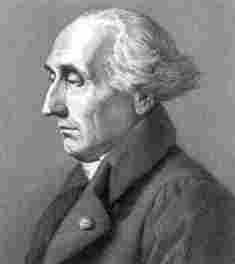
\includegraphics[width=0.3\textwidth,height=\textheight]{fig/Lagrange.jpg}
\caption[\label{fig:Lagrange} Joseph-Louis Lagrange (1736-1813)]{\label{fig:Lagrange} Joseph-Louis Lagrange (1736-1813)\footnotemark{}}
\end{figure}
\footnotetext{Picture is taken from \url{http://www-history.mcs.st-and.ac.uk/history/PictDisplay/Lagrange.html}}

The decision-making process of consumers and producers lies at the core of microeconomic research and is of significant importance for managers. I will not go into detail here, but I will show some examples of how to come to a decision when certain information is given.

Before we come to the Lagrangian multplier method, let me define what (micro)economist mean when they speak of firms and consumers.

A \emph{firm} is a productive unit. In particular, it is an organization that produces goods and services, called the \emph{output}. To do so, it uses inputs called \emph{factors of production}: labor, capital, land, skills, etc. The relationship between the inputs and the output is the production function. The goal of the firm is to achieve whatever goal its owner(s) decide to achieve. Usually, it is (and in Germany, for example, it has to be the case by law) to generate profits, i.e., total revenue minus total cost for the level of production.
Determining the optimal level of production for a firm is a multifaceted decision that encompasses various strategic aspects and is heavily influenced by the market situation of firms. This includes factors such as market power, demand function, production function, cost function, and revenue function.

A consumer is an individual that purchases goods or services to satisfy their needs. They make decisions regarding what to buy, how much to buy in order to maximize their utility. Microeconomists study consumer behavior and factors that influence it, such as prices, income, preferences, and market conditions, to understand the choices consumers make and their impact on markets and the overall economy.

For a deeper understanding of the microeconomic preliminaries related to this topic, please read section \ref{micro-pre} of the appendix.

\begin{figure}
\centering
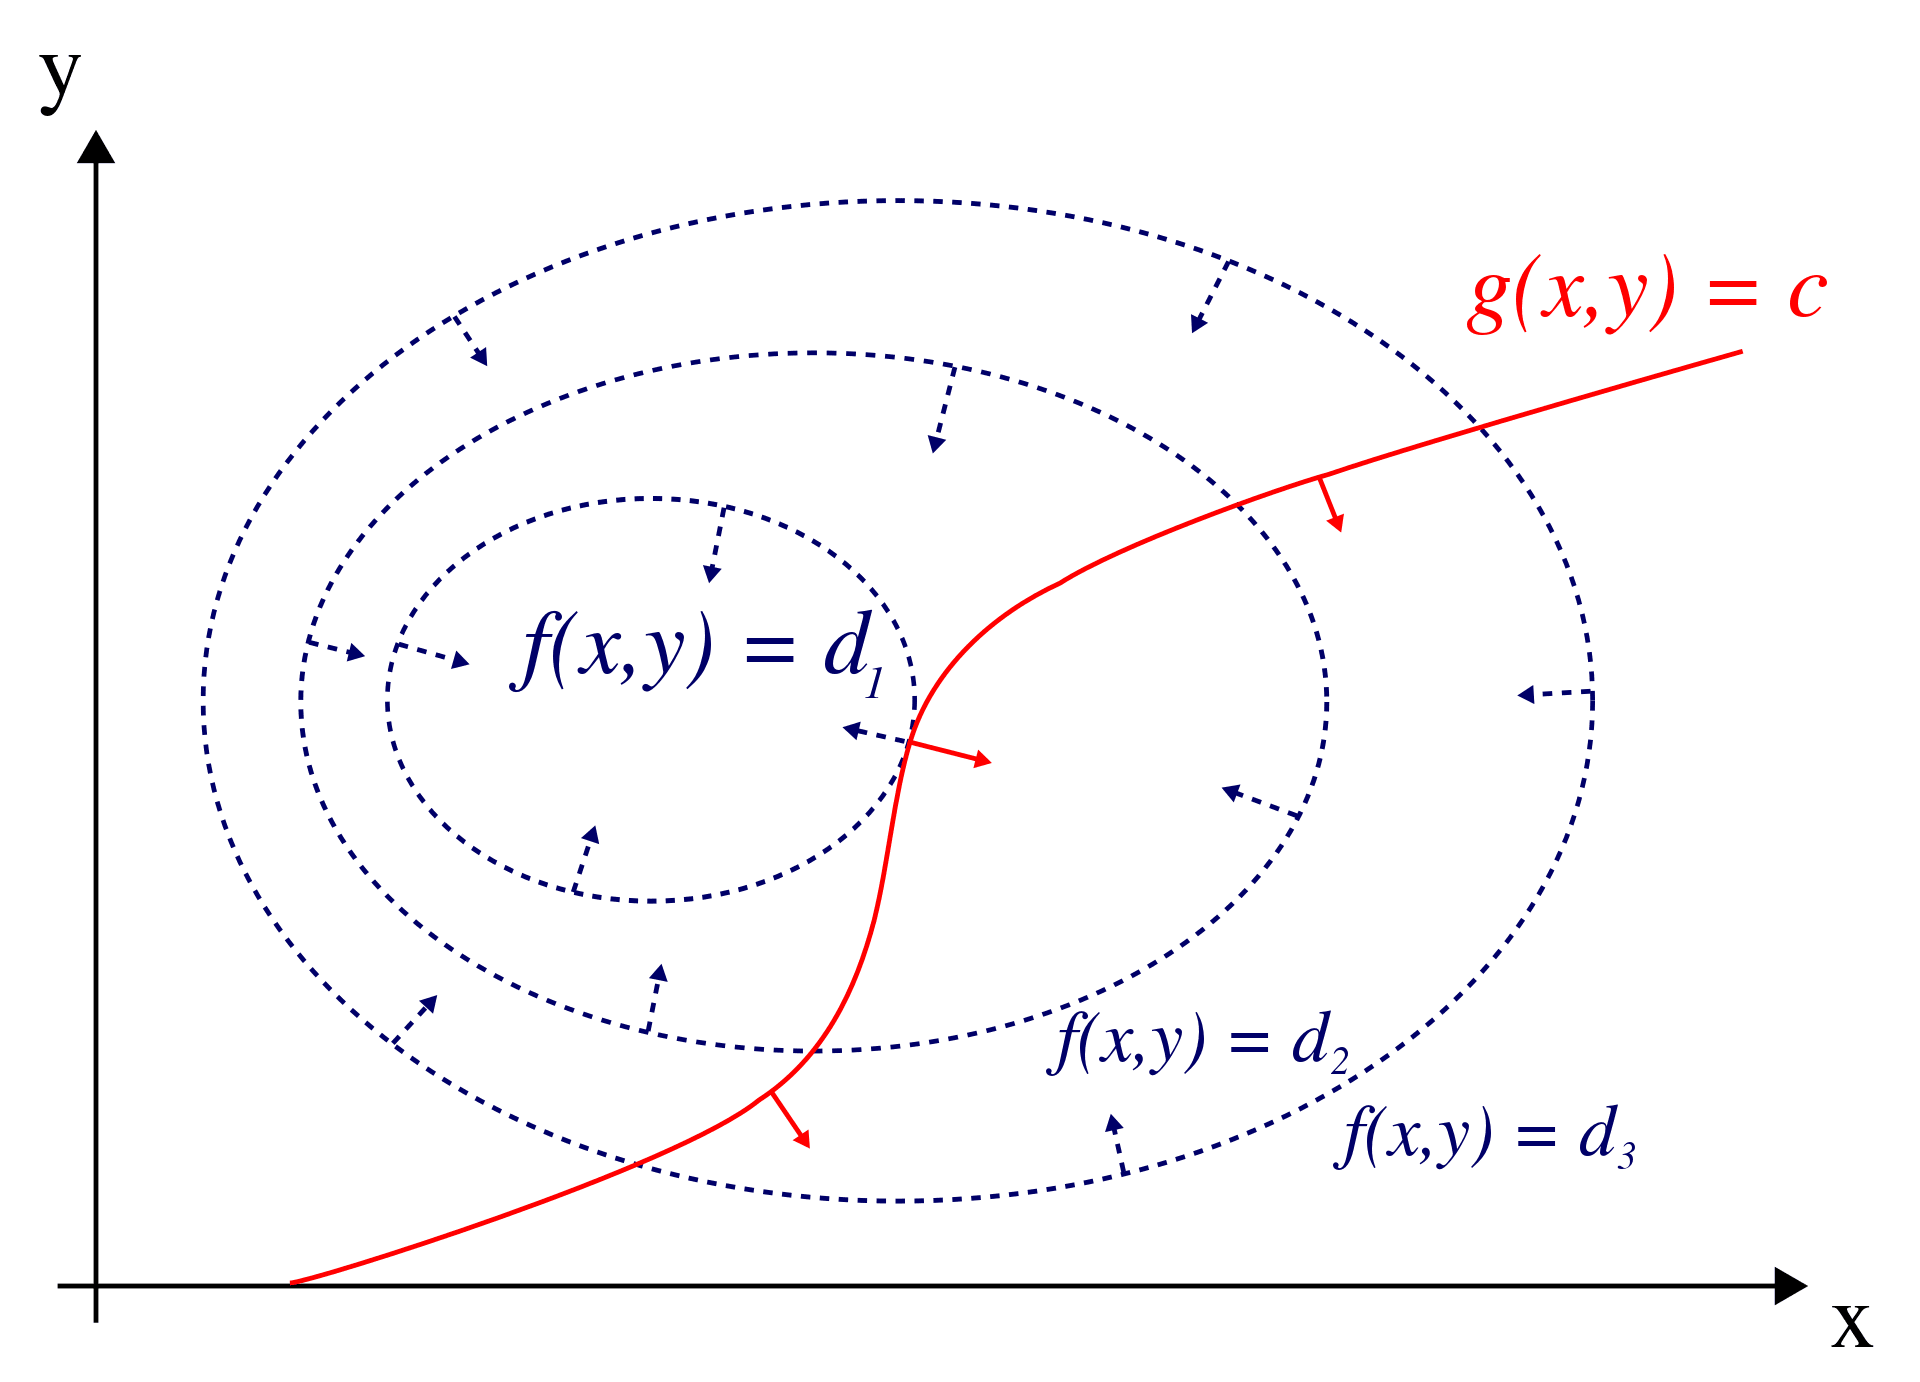
\includegraphics[width=0.7\textwidth,height=\textheight]{fig/lagr2.png}
\caption{\label{fig:lagr2} Contours of the function and the constraint in red}
\end{figure}

The Lagrange multiplier method, named after Joseph-Louis Lagrange,
is a strategy for finding the local maxima and minima of a function subject to constraints.
The red curve in Figure \ref{fig:lagr2} represents the constraint \(g(x, y) = c\),
while the blue curves depict contours of \(f(x, y)\).
The point where the red constraint tangentially intersects a blue contour
represents the maximum of \(f(x, y)\) along the constraint, as \(d1 > d2\).

For a detailed visual explanation of the method, you can watch Dr.~Trefor Bazett's
YouTube video on \href{https://youtu.be/8mjcnxGMwFo}{Lagrange Multipliers \textbar{} Geometric Meaning \& Full Example}, see figure \ref{fig:lagrange-yt}.

\begin{figure}
\centering
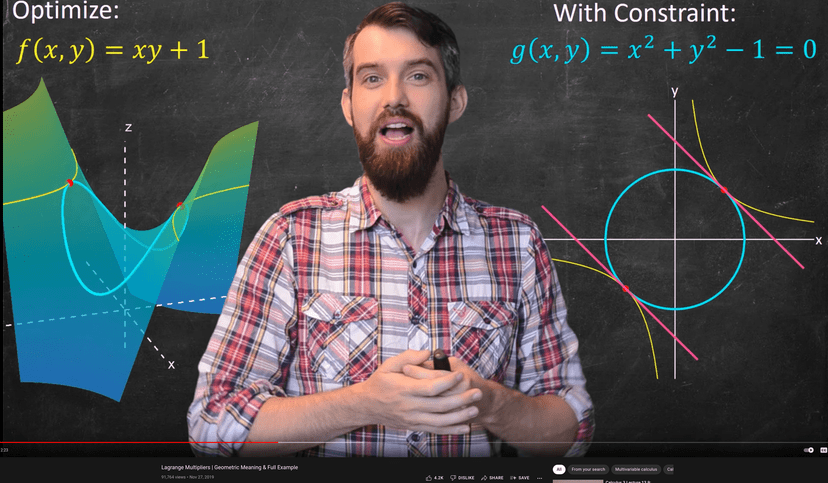
\includegraphics[width=0.4\textwidth,height=\textheight]{fig/lagrange-yt.png}
\caption[\label{fig:lagrange-yt} Lagrange Multiplier graphically explained]{\label{fig:lagrange-yt} Lagrange Multiplier graphically explained\footnotemark{}}
\end{figure}
\footnotetext{This is a snapshot of a YouTube clip, see: \url{https://youtu.be/8mjcnxGMwFo}}

The Lagrange multiplier method, named after Joseph-Louis Lagrange,
is a powerful technique for solving optimization problems with constraints.
It allows us to find the local maxima and minima of a function subject to certain conditions.
The method involves four key steps:

\textbf{Step 1: Formulate the Problem}

Define the problem you want to solve in mathematical terms.
This includes specifying the objective function to be maximized or minimized and the constraints that need to be satisfied.

The problem that we want to solve can be written in the following way,
\[
\begin{array}{ll}
    \max _{x, y} & F(x, y) \\
    \text{ s.t. } & g(x, y)=0
\end{array}
\]
where \(F(x, y)\) is the function to be maximized and \(g(x, y)=0\) is the constraint to be respected.
Notice that \(\max _{x, y}\) means that we must solve (maximize) with respect to \(x\) and \(y\).

\textbf{Step 2: Construct the Lagrangian}

Create a new function called the Lagrangian by combining the objective function
and the constraints using Lagrange multipliers. The Lagrangian introduces new variables,
known as Lagrange multipliers, to account for the constraints.
The Lagrangian, \(\mathcal{L}\), is a combination of the functions that explain the problem:
The \(\lambda\) is called the \emph{Lagrange Multiplier}.
\[
\mathcal{L}(x, y, \lambda)=F(x, y)-\lambda g(x, y)
\]

\textbf{Step 3: Determine the First-Order Conditions}

Differentiate the Lagrangian with respect to the variables of the problem (e.g., x and y)
and the Lagrange multipliers. Set the partial derivatives equal to zero to obtain
the first-order conditions. These conditions represent the necessary conditions for optimality.

Differentiate \(\mathcal{L}\) w.r.t. \(x, y,\) and \(\lambda\) and equate the partial derivatives to 0:
\begin{align*}
    \frac{\partial \mathcal{L}(x, y, \lambda)}{\partial x}=0 & \Leftrightarrow \frac{\partial F(x, y)}{\partial x}-\lambda \frac{\partial g(x, y)}{\partial x}=0 \\
    \frac{\partial \mathcal{L}(x, y, \lambda)}{\partial y}=0 & \Leftrightarrow \frac{\partial F(x, y)}{\partial y}-\lambda \frac{\partial g(x, y)}{\partial y}=0 \\
    \frac{\partial \mathcal{L}(x, y, \lambda)}{\partial \lambda}=0 & \Leftrightarrow g(x, y)=0
\end{align*}

\textbf{Step 4: Solve the System of Equations}

Solve the system of equations obtained from the first-order conditions to find the values of the variables and Lagrange multipliers that satisfy the optimality conditions. The solutions represent the optimal quantities that maximize or minimize the objective function subject to the given constraints.

By following these four steps, you can effectively apply the Lagrange multiplier method to various optimization problems with constraints. It provides a systematic approach to finding the optimal solutions while incorporating the necessary trade-offs imposed by the constraints.

\begin{exercise}
\protect\hypertarget{exr:burgerutility1}{}\label{exr:burgerutility1}Burgers and drinks

Suppose you are in a fast food restaurant and you want to buy burgers and some drinks. You have €12 to spend, a burger costs €3 and a drink costs €2.

\begin{enumerate}
\def\labelenumi{\alph{enumi})}
\tightlist
\item
  Assume that you want to spend all your money and that you can only buy complete units of each products. What are the possible choices of consumption?
\item
  Given your utility function \(U(x,y)=B^{0.6}D^{0.4}\) calculate for each possible consumption point your overall utility. How will you decide?
\item
  Assume that you want to spend all your money and that both products can be bought on a metric scale where one burger weights 200 grams and a drink is 200 ml. How much of both goods would you consume now? Hint: Use the Lagrangian multiplier method.\footnote{Also see: \url{http://www.sfu.ca/~wainwrig/5701/notes-lagrange.pdf}}
\end{enumerate}

Please find solution to the exercise \protect\hyperlink{sol:burgerutility1}{in the appendix.}
\end{exercise}

\begin{exercise}
\protect\hypertarget{exr:lama}{}\label{exr:lama}Labor and machines

Suppose you rent a factory for a month to produce as many masks as possible. After you have paid the rent, you need to decide how many machines to buy and how many workers to hire for the given month.

What is the optimal amount of workers and machines to employ for the given month, if you assume the following:

\begin{itemize}
\tightlist
\item
  \(L\) denotes the number of workers
\item
  \(K\) denotes the number of machines
\item
  \(Q\) denotes the number of masks produced
\item
  \(p_L\) denotes the price of a worker for a month
\item
  \(p_K\) denotes the price of a machine for a month
\item
  \(B\) denotes the money you can invest in the production of masks for the next month
\item
  \(B = 216\)
\item
  The production of masks can be explained by the following Cobb-Douglas production function: \(Q = K^{0.4}L^{0.6}\)
\item
  \(p_L = 2\)
\item
  \(p_K = 8\)
\end{itemize}

Please find solution to the exercise \protect\hyperlink{sol:lama}{in the appendix.}
\end{exercise}

\begin{exercise}
\protect\hypertarget{exr:cchoice}{}\label{exr:cchoice}Consumption choice

Suppose you want to spend your complete budget of €30, \[I=30,\] on the
consumption of two goods, \(A\) and \(B\). Further assume good \(A\) costs €6, \[p_A=6,\]
and good \(B\) costs €4, \[p_B=4\] and that you want to maximize your utility that
stems from consuming the two goods.
Calculate how much of both goods to buy and consume, respectively, when your utility function
is given as \[U(A,B)=A^{0.8}B^{0.2}\]

Please find solution to the exercise \protect\hyperlink{sol:cchoice}{in the appendix.}
\end{exercise}

\begin{exercise}
\protect\hypertarget{exr:costmin}{}\label{exr:costmin}Cost-minimizing combination of factors

Using two input factors \(r_1\) and \(r_2\), a firm wants to produces a fixed quantity of a product, that is \(x=20\). Given the production function
\[
    x=\frac{5}{4} r_1^{\frac{1}{2}} r_2^{\frac{1}{2}}
    \] and the factor prices
\[
    p_{r_1}=1 \quad \text{ and } p_{r_2}=4.
    \]
calculate the cost-minimizing combination of factors (\(r_1, r_2\)).

Please find solution to the exercise \protect\hyperlink{sol:costmin}{in the appendix.}
\end{exercise}

\begin{exercise}
\protect\hypertarget{exr:lagrcons}{}\label{exr:lagrcons}Lagrange with n-constraints

Write down the Lagrangian multiplier for the following minimization problem:

Minimize \(f(\mathbf{x})\) subject to:
\[\begin{aligned}
    g_1(\mathbf{x})&=0 \\
    g_2(\mathbf{x})&=0\\
    &\vdots\\
    g_n(\mathbf{x})&=0,\end{aligned}\]
where \(n\) denotes the number of constraints.
\end{exercise}

Please find solution to the exercise \protect\hyperlink{sol:lagrcons}{in the appendix.}

\hypertarget{decision-making-under-uncertainty}{%
\section{Decision making under uncertainty}\label{decision-making-under-uncertainty}}

When it comes to decision-making under uncertainty you need to have a criterion that helps you to come to a \emph{rational} decision. The choice of criteria is a matter of taste and should at best fit with overall (business) strategy.

\hypertarget{laplace-criterion}{%
\subsection*{Laplace criterion}\label{laplace-criterion}}

In case of different possible states of nature and no information on their probability of occurrences, the Laplace criterion simply assigns equal probabilities to the possible pay offs for each action and then selecting that alternative which corresponds to the maximum \emph{expected} pay off. An example is given in \citet{Finne1998three}.

\hypertarget{maximax-criterion-go-for-cup}{%
\subsection*{Maximax criterion (go for cup)}\label{maximax-criterion-go-for-cup}}

If you like to \emph{go for cup}, i.e., like to have the best out of the best possible outcome without taking into consideration the fact that this may potentially also result in the worst possible scenario, then, you can choose the alternative that gives the maximum possible output.

\hypertarget{minimax-criterion-best-of-the-worst}{%
\subsection*{Minimax criterion (best of the worst)}\label{minimax-criterion-best-of-the-worst}}

The Minimax (or maximin) criterion is a conservative criterion because it is based on making the best out of the worst possible conditions. Again, examples on how to calculate it are given in \citet{Finne1998three}..

\hypertarget{savage-minimax-criterion}{%
\subsection*{Savage Minimax criterion}\label{savage-minimax-criterion}}

This criterion aims to minimize the worst-case regret to perform as closely as possible to the optimal course. Since the minimax criterion applied here is to the regret (difference or ratio of the payoffs) rather than to the payoff itself, it is not as pessimistic as the ordinary minimax approach. For more details, please read \citet{Finne1998three}.

\hypertarget{hurwicz-criterion}{%
\subsection*{Hurwicz criterion}\label{hurwicz-criterion}}

The Hurwicz criterion allows the decision maker to calculates a weighted average between the best and worst possible payoff for each decision alternative. Then, the alternative with the maximum weighted average is chosen.

For each decision alternative, the weight \(\alpha\) is used to compute Hurwicz the value:
\[H_i=\alpha \cdot \overline{O}_i + (1-\alpha)\cdot \underline{O}_i\]
where \(\overline{O}_i=\max_{j=1,\dots,p}{O_{ij}}\qquad \forall i\) and \(\underline{O}_i=\min_{j=1,\dots,p}{O_{ij}}\qquad \forall i\), i.e., the respective maximum and minimum Output for each alternative, \(i\).
The example that is shown in Figure 7 of \citet[p.401]{Finne1998three} contains some errors. Here is the \emph{correct table} including the Hurwicz-values (we assume a \(\alpha=.5\)):

\begin{longtable}[]{@{}lccc@{}}
\toprule\noalign{}
\(O_{ij}\) & \(min(\theta_1)\) & \(max(\theta_2)\) & \(H_i\) \\
\midrule\noalign{}
\endhead
\bottomrule\noalign{}
\endlastfoot
\(a_1\) & 36 & 110 & 73 \\
\(a_2\) & 40 & 100 & 70 \\
\(a_3\) & 58 & 74 & 66 \\
\(a_4\) & 61 & 66 & 63.5 \\
\end{longtable}

Thus, the order of preference is \(a_4\succ a_3 \succ a_1 \succ a_2\).

\begin{exercise}
\protect\hypertarget{exr:finne}{}\label{exr:finne}

Three categories

Read \citet{Finne1998three} and answer the following questions:

\begin{enumerate}
\def\labelenumi{\alph{enumi})}
\tightlist
\item
  Explain the three categories of decision making.
\item
  Give examples of the three categories of decision making.
\item
  Explain the four criteria for decision making under uncertainty.
\end{enumerate}

\end{exercise}

\hypertarget{decision-making-under-risk}{%
\section{Decision making under risk}\label{decision-making-under-risk}}

When some information is given about the probability of occurrence of states of nature, we speak of \emph{decision-making under risk}. The most straight forward technique to make a decision here is to maximize the expected outcome for each alternative given the probability of occurrence, \(p_j\).

However, the expected utility hypothesis states that the subjective value associated with an individual's gamble is the statistical expectation of that individual's valuations of the outcomes of that gamble, where these valuations may differ from the Euro value of those outcomes. Thus, you should better look on the utility of a respective outcome rather than on the outcome itself because the utility and outcome do not have to be linked in a linear way. The St.~Petersburg Paradox by Daniel Bernoulli in 1738 is considered the beginnings of the hypothesis.

\hypertarget{st.-petersburg-paradox}{%
\subsection{St.~Petersburg Paradox}\label{st.-petersburg-paradox}}

\hypertarget{ininite-st.-petersburg-lotteries}{%
\subsubsection{Ininite St.~Petersburg lotteries}\label{ininite-st.-petersburg-lotteries}}

Suppose a casino offers a game of chance for a single player, where a fair coin is tossed at each stage. The first time head appears the player gets \$1. From then onwards, every time a head appears, the stake is doubled. The game continues until the first tails appears, at which point the player receives \(\$ 2^{k-1}\), where k is the number of tosses (number of heads) plus one (for the final tails).
For instance, if tails appears on the first toss, the player wins \$0. If tails appears on the second toss, the player wins \$2. If tails appears on the third toss, the player wins \$4, and so on. The extensive form of the game is given in figure \ref{fig:spextensiveform}.

\begin{figure}
\centering
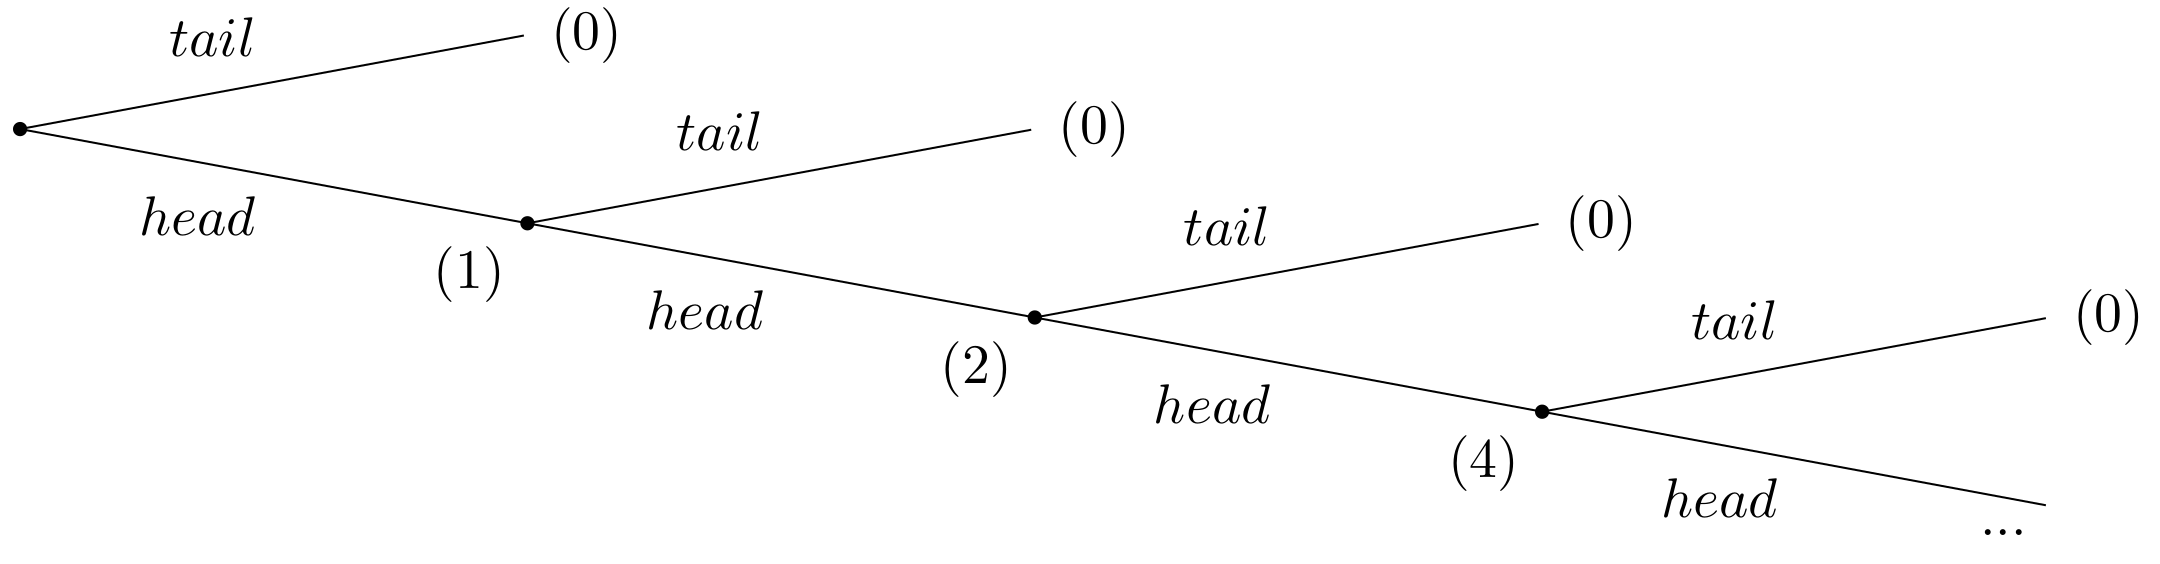
\includegraphics[width=0.8\textwidth,height=\textheight]{fig/spextensiveform.png}
\caption{\label{fig:spextensiveform} Extensive form of the St.~Petersburg paradox}
\end{figure}

Given the rules of the game, what would be a fair price for the player to pay the casino in order to enter the game?

To answer this question, one needs to consider the expected payout: The player has a 1/2 probability of winning \$1, a 1/4 probability of winning \$2, a 1/8 probability of winning \$4, and so on. Thus, the overall expected value can be calculated as follows:
\[
E = \frac{1}{2} \cdot 1 + \frac{1}{4} \cdot 2 + \frac{1}{8} \cdot 4+ \frac{1}{16} \cdot 8 + \dots 
\]
This can be simplified as:
\[
E = \frac{1}{2} + \frac{1}{2} + \frac{1}{2} + \frac{1}{2} + \dots = + \infty.
\]
That means the expected win for playing this game is an infinite amount of money. Based on the expected value, a risk-neutral individual should be willing to play the game at any price if given the opportunity.
The willingness to pay of most people who have given the opportunity to play the game deviates dramatically from the objectively calculable expected payout of the lottery. This describes the apparent paradox.

In the context of the St.~Petersburg Paradox, it becomes evident that relying solely on expected values is inadequate for certain games and for making well-informed decisions. Expected utility, on the other hand, has been the prevailing concept used to reconcile actual behavior with the notion of rationality thus far.

\hypertarget{finite-st.-petersburg-lotteries}{%
\subsubsection*{Finite St.~Petersburg lotteries}\label{finite-st.-petersburg-lotteries}}
\addcontentsline{toc}{subsubsection}{Finite St.~Petersburg lotteries}

Let us assume that at the beginning, the casino and the player agrees upon how many times the coin will be tossed. So we have a finite number I of lotteries with \(1 \leq I \leq \infty\).

To calculate the expected value of the game, the probability \(p(i)\) of throwing any number \(i\) of consecutive head is crucial. This probability is given by
\[
p(i)=\underbrace{\frac{1}{2} \cdot \frac{1}{2} \cdot \cdots \frac{1}{2}}_{i \text { factors}}=\frac{1}{2^{i}}
\]
The payoff \(W(I)\) is, if head appears \(I\)-times in a row by
\[
W(I)=2^{I-1}
\]
The expected payoff \(E(W(I))\) if the coin is flipped \(I\) times is then given by
\[
E(W(I))=\sum_{i=1}^{I} p(i) \cdot W(i)=\sum_{i=1}^{I} \frac{1}{2^{i}} \cdot 2^{i-1}=\sum_{i=1}^{I} \frac{1}{2}=\frac{I}{2}
\]

Thus, the expected payoff grows proportionally with the maximum number of rolls. This is because at any point in the game, the option to keep playing has a positive value no matter how many times head has appeared before.
Thus, the expected value of the game is infinitely high for an unlimited number of tosses but not so for a limited number of tosses. Even with a very limited maximum number of tosses of, for example, \(I = 100\), only a few players would be willing to pay
\$50 for participation. The relatively high probability to leave the game with no or very low winnings leads in general to a subjective rather low evaluation that is below the expected value.

In the real world, we understand that money is limited and the casino offering this game also operates within a limited budget.
Let's assume, for example, that the casino's maximum budget is \$20,000,000. As a result, the game must conclude after 25 coin tosses because \(2^{25} = 33,554,432\) would exceed the casino's financial capacity. Consequently, the expected value of the game in this scenario would be significantly reduced to just \$12.50.
Interestingly, if you were to ask people, most would still be willing to pay less than \$12.50 to participate. How can we explain this? Well, it is not the expected outcome that matters but the utility that stems from the outcome.

\hypertarget{the-impact-of-output-on-utility-matters}{%
\subsubsection{The impact of output on utility matters}\label{the-impact-of-output-on-utility-matters}}

\emph{Daniel Bernoulli} (1700 - 1782) worked on the paradox while being a professor in St.~Petersburg. His solution builds on the conceptual separation of the expected payoff and its utility. He describes the basis of the paradox as follows:

\begin{quote}
``Until now scientists have usually rested their hypothesis on the assumption that all gains must be evaluated exclusively in terms of themselves, i.e., on the basis of their intrinsic qualities, and that these gains will always produce a utility directly proportionate to the gain.'\,' \citep[p.~27]{Bernoulli1954Exposition}
\end{quote}

The relationship between gain and utility, however, is not simply directly proportional but rather more complex. Therefore, it is important to evaluate the game based on expected utility rather than just the expected payoff.
\[
E(u(W(I)))=\sum_{i=1}^{I} p(i) \cdot u(W(i))=\sum_{i=1}^{I} \frac{1}{2^{i}} \cdot u\left(2^{i-1}\right)
\]
Daniel Bernoulli himself proposed the following logarithmic utility function:
\[
u(W)=a \cdot \ln (W),
\]
where \(a\) is a positive constant. Using this function in the expected utility, we get
\[
E(u(W(I)))=\sum_{i=1}^{I} \frac{1}{2^{i}} \cdot a \cdot \ln \left(2^{i-1}\right)=a \cdot \sum_{i=1}^{I} \frac{i-1}{2^{i}} \ln 2=a \cdot \ln 2 \cdot \sum_{i=1}^{I} \frac{i-1}{2^{i}}.
\]
The infinite series, \(\sum_{i=1}^{I} \frac{i-1}{2^{i}}\), converges to 1 (\(\lim _{I \rightarrow \infty} \sum_{i=1}^{I} \frac{i-1}{2^{i}}=1\)). Thus, given an ex ante unbounded number of throws, the expected utility of the game is given by
\[
E(u(W(\infty)))=a \cdot \ln 2 .
\]

In experiments in which people were offered this game, their willingness to pay was roughly between 2 and 3 Euro. Thus, the suggests logarithmic utility function seems to be a pretty realistic specification.
The main reason is mathematically that the increasing expected payoff has decreasing marginal utility and hence the utility function reflects the risk aversion of many people.

\begin{exercise}
\protect\hypertarget{exr:ratrisk}{}\label{exr:ratrisk}

Rationality and risk

There are 90 balls in an box. It is known that 30 of them are red, the remaining 60 are blue or green. An individual can choose between the following lotteries:

\begin{longtable}[]{@{}
  >{\centering\arraybackslash}p{(\columnwidth - 4\tabcolsep) * \real{0.3333}}
  >{\centering\arraybackslash}p{(\columnwidth - 4\tabcolsep) * \real{0.3333}}
  >{\centering\arraybackslash}p{(\columnwidth - 4\tabcolsep) * \real{0.3333}}@{}}
\toprule\noalign{}
\begin{minipage}[b]{\linewidth}\centering
\end{minipage} & \begin{minipage}[b]{\linewidth}\centering
Payoff
\end{minipage} & \begin{minipage}[b]{\linewidth}\centering
probability
\end{minipage} \\
\midrule\noalign{}
\endhead
\bottomrule\noalign{}
\endlastfoot
Lottery 1 & 100 Euro if a red ball is drawn 0 Euro else & \(p=\frac{1}{3}\) \\
Lottery 2 & 100 Euro if a blue ball is drawn 0 Euro else & \(0 \leq p \leq \frac{2}{3}\) \\
\end{longtable}

In a second variant it has the choice between the following lotteries:

\begin{longtable}[]{@{}
  >{\raggedright\arraybackslash}p{(\columnwidth - 4\tabcolsep) * \real{0.3333}}
  >{\raggedright\arraybackslash}p{(\columnwidth - 4\tabcolsep) * \real{0.3333}}
  >{\raggedright\arraybackslash}p{(\columnwidth - 4\tabcolsep) * \real{0.3333}}@{}}
\toprule\noalign{}
\begin{minipage}[b]{\linewidth}\raggedright
\end{minipage} & \begin{minipage}[b]{\linewidth}\raggedright
Payoff
\end{minipage} & \begin{minipage}[b]{\linewidth}\raggedright
probability
\end{minipage} \\
\midrule\noalign{}
\endhead
\bottomrule\noalign{}
\endlastfoot
Lottery 3 & 100 Euro if a red or green ball is drawn or 0 Euro else & \(\frac{1}{3} \leq p \leq 1\) \\
Lottery 4 & 100 Euro if a blue or green ball is drawn or 0 Euro else & \(p=\frac{2}{3}\) \\
\end{longtable}

\begin{enumerate}
\def\labelenumi{\alph{enumi})}
\tightlist
\item
  Which of the lotteries does the individual choose on the basis of expected values (risk neutral)?
\item
  Which of the lotteries does the individual choose on the basis of expected utility if the utility of a payoff of \(x\) is given by \(u(x) = x^2\)?
\item
  Empirical studies, e.g.~\cite{Camerer1992Recent}, show, however, that most individuals will usually choose lotteries 1 and 4. will. Discuss: Is this consistent with rational behavior?
\end{enumerate}

\end{exercise}

\hypertarget{decision-making-with-conditional-probabilities-bayes-theorem}{%
\section{Decision making with conditional probabilities (Bayes' theorem)}\label{decision-making-with-conditional-probabilities-bayes-theorem}}

\begin{center}\rule{0.5\linewidth}{0.5pt}\end{center}

After successful completion of the module, students are able to:

\begin{itemize}
\tightlist
\item
  Understand and use the terminology of probability.
\item
  Determine whether two events are mutually exclusive and whether two events are independent.
\item
  Calculate probabilities using the addition rules and multiplication rules.
\item
  Calculate with conditional probabilities using Bayes Theorem.
\item
  Construct and interpret venn and tree diagrams.
\item
  Apply their knowledge of probability theory to decision making in business.
\end{itemize}

\begin{center}\rule{0.5\linewidth}{0.5pt}\end{center}

\begin{figure}
\centering
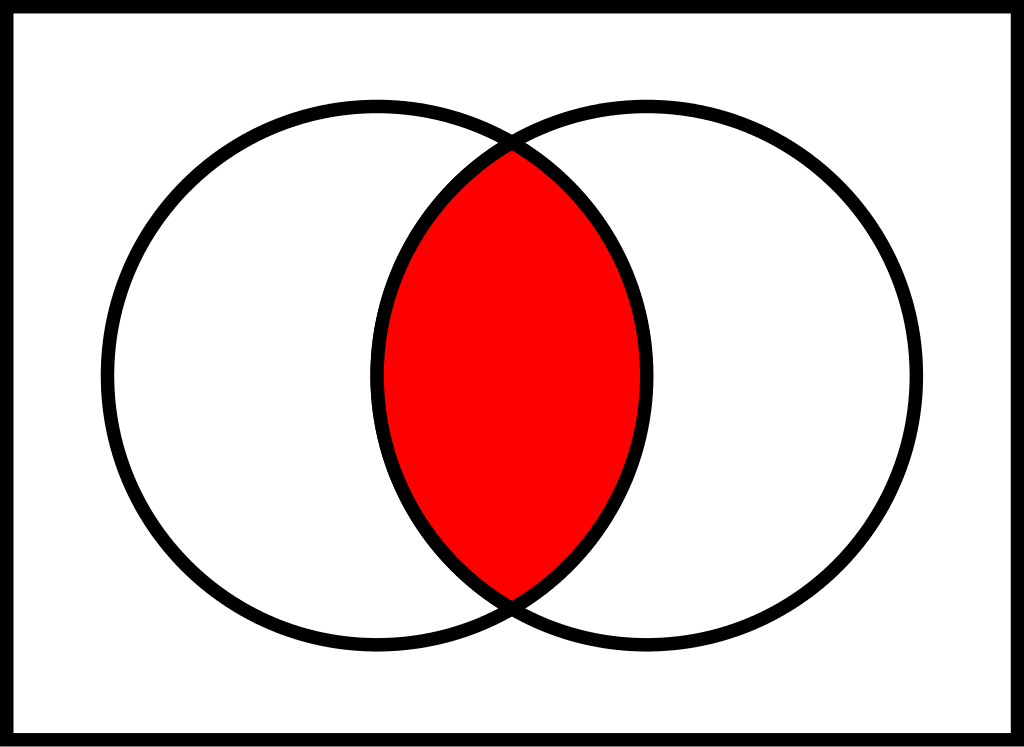
\includegraphics[width=0.3\textwidth,height=\textheight]{fig/intersection.png}
\caption{\label{fig:afig} Intersection: \(A \cap B\)}
\end{figure}

\begin{figure}
\centering
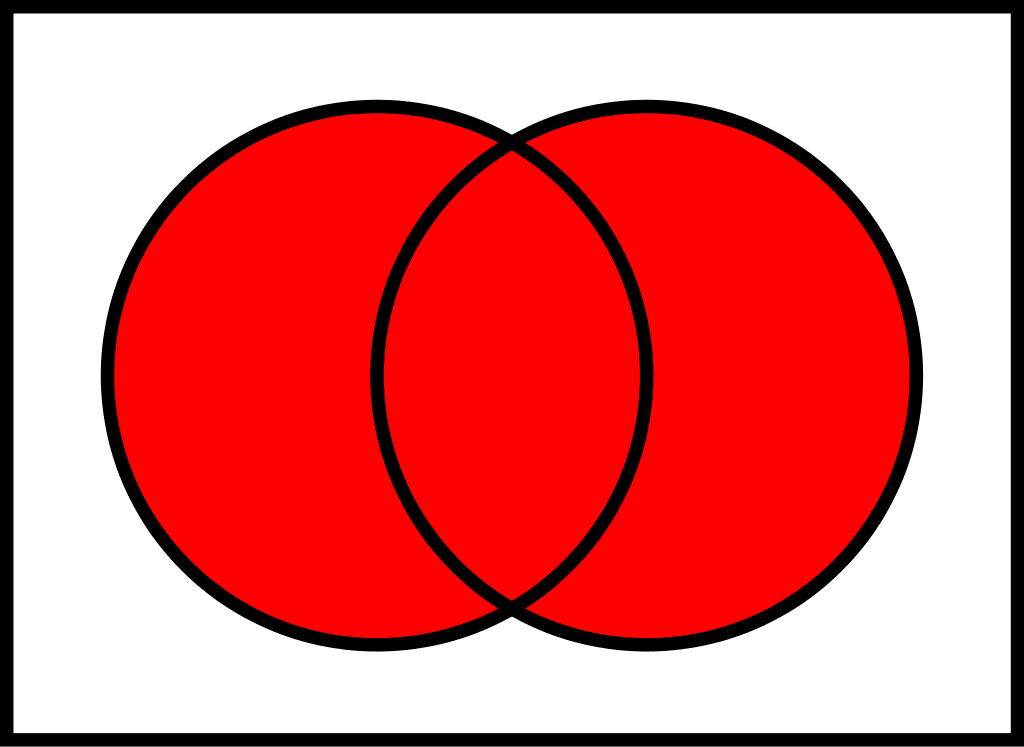
\includegraphics[width=0.3\textwidth,height=\textheight]{fig/union.png}
\caption{\label{fig:bfig} Union: \(A \cup B\)}
\end{figure}

\begin{figure}
\centering
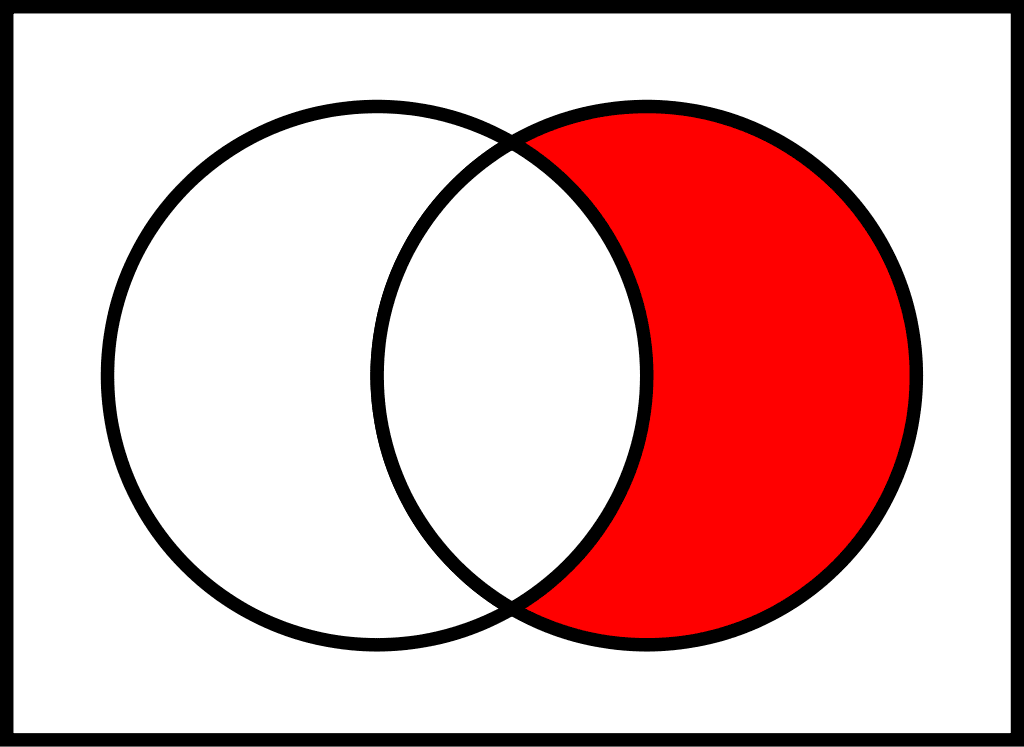
\includegraphics[width=0.3\textwidth,height=\textheight]{fig/notA.png}
\caption{\label{fig:cfig} Relative complement: \(\neg A \cup B\)}
\end{figure}

\hypertarget{school-stuff}{%
\subsubsection*{School Stuff}\label{school-stuff}}

The next chapter will deal with stochastics. In Germany, stochastics is taught in the Gymnasium. If you are not from Germany, it was probably also part of your school experience. When I moved to Cologne in 2020, I found the following page shown in figure \ref{fig:inschool} that I had received from my high school math teacher. It was September 1993 and I was a desperate fifth grader in my fourth week. Perhaps you'd like to share your experiences with stochastics?

\begin{figure}
\centering
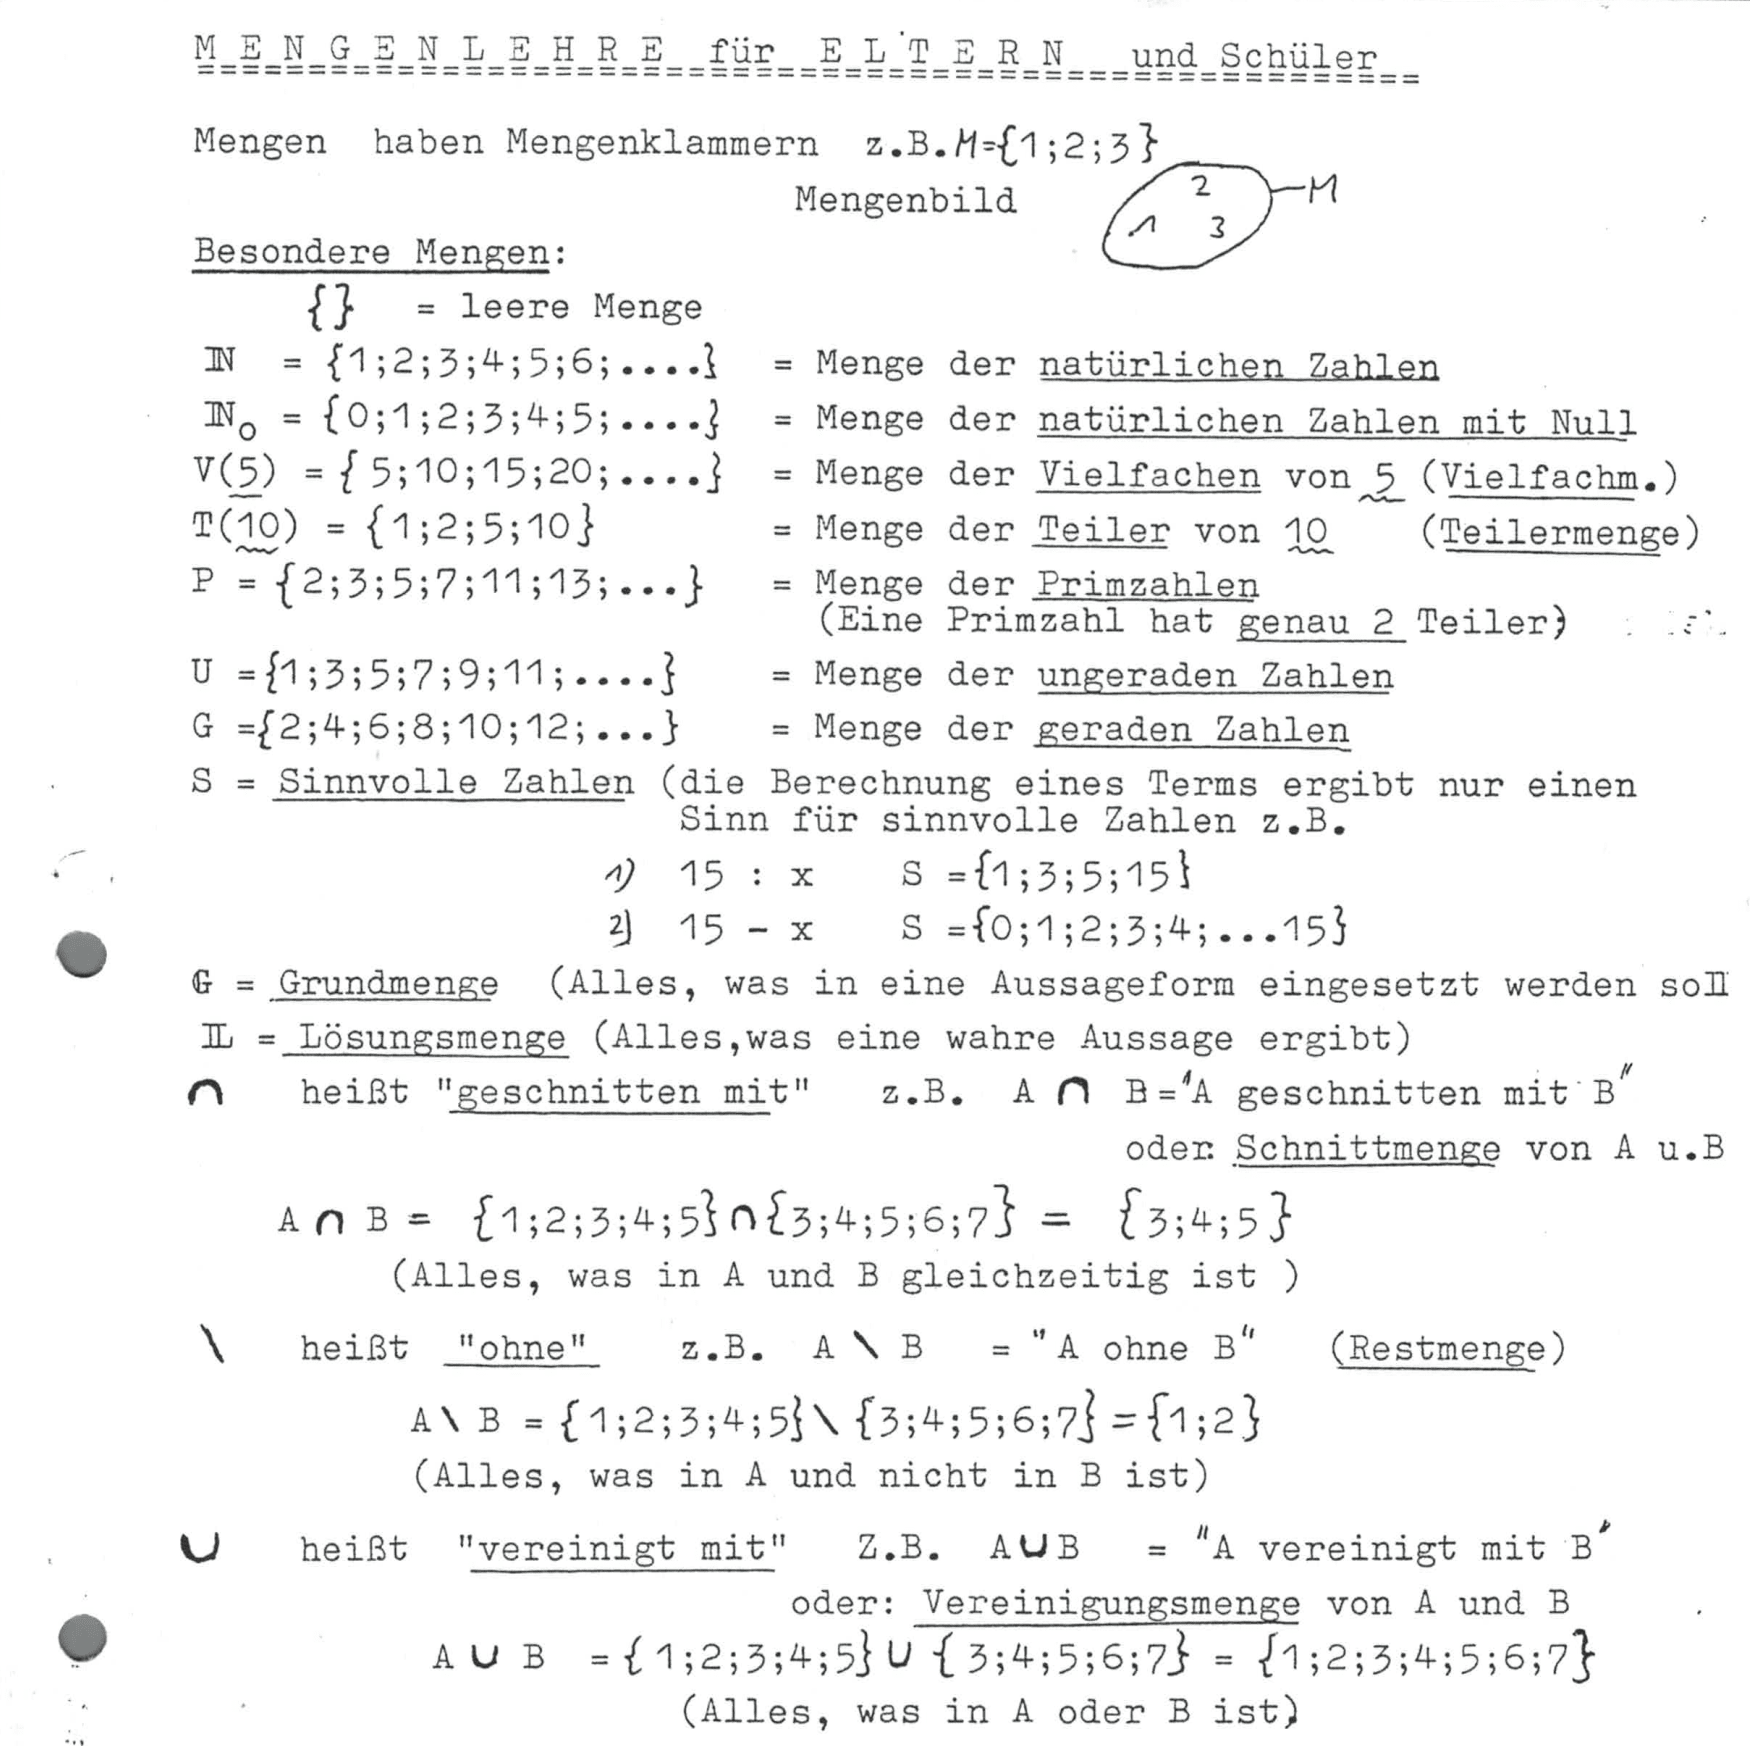
\includegraphics[width=0.9\textwidth,height=\textheight]{fig/mengenlehre-5.png}
\caption{\label{fig:inschool} Relative complement: \(\neg A \cup B\)}
\end{figure}

\hypertarget{terminology-pa-pab-omega-cap-neg}{%
\subsection{\texorpdfstring{Terminology: \(P(A)\), \(P(A|B)\), \(\Omega\), \(\cap\), \(\neg\), \ldots{}}{Terminology: P(A), P(A\textbar B), \textbackslash Omega, \textbackslash cap, \textbackslash neg, \ldots{}}}\label{terminology-pa-pab-omega-cap-neg}}

\hypertarget{sample-space}{%
\subsubsection{Sample space}\label{sample-space}}

A result of an \emph{experiment} is called an \emph{outcome}. An experiment is a planned operation carried out under controlled conditions. Flipping a fair coin twice is an example of an experiment.
The \emph{sample space} of an experiment is the set of all possible outcomes.
The Greek letter \(\Omega\) is often used to denote the sample space. For example, if you flip a fair coin, \(\Omega = \{H, T\}\) where the outcomes heads and tails are denoted with \(H\) and \(T\), respectively.

\textbf{Example: Sample space}
Find the sample space for the following experiments:

\begin{enumerate}
\def\labelenumi{\alph{enumi})}
\tightlist
\item
  One coin is tossed.
\item
  Two coins are tossed once.
\item
  Two dices are tossed once.
\item
  Picking two marbles, one at a time, from a bag that contains many blue, \(B\), and red marbles, \(R\).
\end{enumerate}

\textbf{Solutions:}

\begin{enumerate}
\def\labelenumi{\alph{enumi})}
\tightlist
\item
  \(\Omega = \{head, tail\}\)
\item
  \(\Omega = \{(head, head), (tail, tail),(head, tail),(tail, head)\}\)
\item
  Overall, 36 different outcomes:
  \(\{  (1,1),(1,2),(1,3),(1,4),(1,5),(1,6),(2,1),(2,2),\dots,(6,6)  \}\)
\item
  \(\Omega = \{(B,B), (B,R), (R,B), (R,R)\}\).
\end{enumerate}

Overall, there are three ways to represent a sample space:

\begin{enumerate}
\def\labelenumi{\arabic{enumi}.}
\tightlist
\item
  to list the possible outcomes (see example above),
\item
  to create a tree diagram (see \ref{fig:decisiontree}), or
\item
  to create a Venn diagram (see \ref{fig:venndiagramm}).
\end{enumerate}

\begin{figure}
\centering
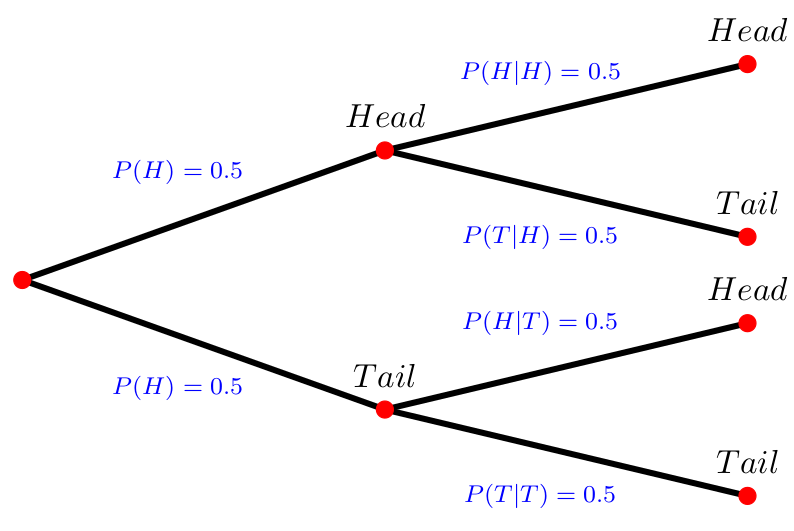
\includegraphics[width=0.5\textwidth,height=\textheight]{fig/treedia.png}
\caption{\label{fig:decisiontree} Tree diagramm}
\end{figure}

\begin{figure}
\centering
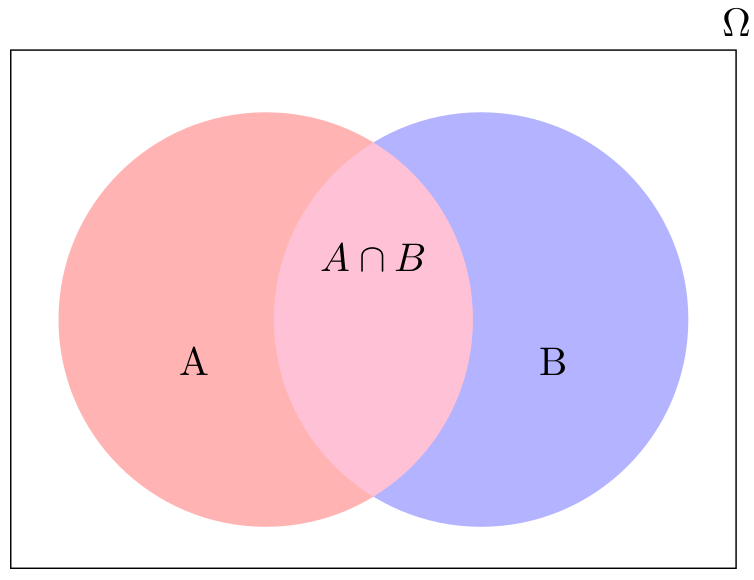
\includegraphics[width=0.25\textwidth,height=\textheight]{fig/venndia.png}
\caption{\label{fig:venndiagramm} Venn diagramm}
\end{figure}

\hypertarget{probability}{%
\subsubsection{Probability}\label{probability}}

Probability is a measure that is associated with how certain we are of outcomes of a particular experiment or activity. The probability of an event \(A\), written \(P(A)\), is defined as
\[
P(A)=\frac{\text{Number of outcomes favorable to the occurrence of } A}{\text{Total number of equally likely outcomes}}=\frac{n(A)}{n(\Omega)}
\]
For example, A dice has 6 sides with 6 different numbers on it. In particular, the set of \emph{elements} of a dice is \(M=\{1,2,3,4,5,6\}\). Thus, the probability to receive a 6 is 1/6 because we look for one wanted outcome in six possible outcomes.

\textbf{Example: Probability}

When a fair dice is thrown, what is the probability of getting

\begin{enumerate}
\def\labelenumi{\alph{enumi})}
\tightlist
\item
  the number 5,
\item
  a number that is a multiple of 3,
\item
  a number that is greater than 6,
\item
  a positive number that is less than 7.
\end{enumerate}

\textbf{Solutions:} A fair dice is an unbiased dice where each of the six numbers is equally likely to turn up. The sample space is \(\Omega = \{1, 2, 3, 4, 5, 6\}\).

\begin{enumerate}
\def\labelenumi{\alph{enumi})}
\tightlist
\item
  Let A be the event of getting the number 5, \(A=\{5\}\). Then, \(P(A)=\frac{1}{6}\).
\item
  Let \(B\) be the event of getting a multiple of 3, \(B=\{3, 6\}\). Then, \(P(B)=\frac{1}{3}\).
\item
  Let \(C\) be the event of getting a number greater than 6, \(C=7,8,\dots\). Then, \(P(C)=0\) as there is no number greater than 6 in the sample space \(\Omega=\{1,2,3,4,5,6\}\). A probability of 0 means the event will never occur.
\item
  Let D be the event of getting a number less than 7, \(D=\{1,2,3,4,5,6\}\). Then, \(P=1\) as the event will always occur.
\end{enumerate}

\hypertarget{the-complement-of-an-event-neg-event}{%
\subsubsection{\texorpdfstring{The complement of an event (\(\neg-Event\))}{The complement of an event (\textbackslash neg-Event)}}\label{the-complement-of-an-event-neg-event}}

The complement of event \(A\) is denoted with a \(\neg A\) or sometimes with a superscript `c' like \(A^c\).
It consists of all outcomes that are \emph{not} in \(A\). Thus, it should be clear that \(P(A) + P(\neg A) = 1\).
For example, let the sample space be \(\Omega = \{1, 2, 3, 4, 5, 6\}\) and let \(A = \{1, 2, 3, 4\}\).
Then, \(\neg A = \{5, 6\}\); \(P(A) = \frac{4}{6}\); \(P(\neg A) = \frac{2}{6}\); and \(P(A) + P(\neg A) = \frac{4}{6}+\frac{2}{6} = 1\).

\hypertarget{independent-events-and-events}{%
\subsubsection{Independent events (AND-events)}\label{independent-events-and-events}}

Two events are independent when the outcome of the first event does not influence the outcome of the second event.
For example, if you throw a dice and a coin, the number on the dice does not affect whether the result you get on the coin.
More formally, two events are independent if the following are true:
\begin{align*}
    P(A|B) &= P(A)\\
    P(B|A) &= P(B)\\
    P(A \cap B) &= P(A)P(B)
\end{align*}

To calculate the probability of two independent events (\(X\) and \(Y\)) happen, the probability of the first event, \(P(X)\), has to be multiplied with the probability of the second event, \(P(Y)\):
\[ P(X \text{ and } Y)=P(X \cap Y)=P(X)\cdot P(Y),\]
where \(\cap\) stands for `and'.
For example, let \(A\) and \(B\) be \(\{1, 2, 3, 4, 5\}\) and \(\{4, 5, 6, 7, 8\}\), respectively. Then \(A \cap B = \{4, 5\}\).

\textbf{Example: Three dices}

Suppose you have three dice. Calculate the probability of getting three times a 4.

\textbf{Solutions:}
The probability of getting a \(4\) on one dice is 1/6. The probability of getting three \(4\) is:
\[
P(4 \cap 4 \cap 4) = \frac{1}{6}\cdot \frac{1}{6}\cdot \frac{1}{6}= \frac{1}{216}
\]

\hypertarget{dependent-events--events}{%
\subsubsection{\texorpdfstring{Dependent events (\(|\)-Events)}{Dependent events (\textbar-Events)}}\label{dependent-events--events}}

Events are dependent when one event affects the outcome of the other. If \(A\) and \(B\) are dependent events then the probability of both occurring is the product of the probability of \(A\) and the probability of \(A\) \emph{after} \(B\) has occurred:
\begin{align*}
    P(A \cap B)&=P(A)\cdot P(B|A),\\
    \Leftrightarrow P(B|A)&=\frac{P(A \cap B)}{P(A)}\cdot 
\end{align*}
where \(|A\) stands for \texttt{after\ A\ has\ occurred\textquotesingle{},\ or}given A has occurred'. In other words, \(P(B|A)\) is the probability of \(B\) given \(A\). This equation is also known as the \textbf{Multiplication Rule}.

The conditional probability of A given B is written \(P(A|B)\). \(P(A|B)\) is the probability that event A will occur given that the event B has already occurred. A conditional reduces the sample space. We calculate the probability of A from the reduced sample space B. The formula to calculate \(P(A|B)\) is \[ P(A|B) = \frac{P\left(A\cap B\right)}{P\left(B\right)}\] where \(P(B)\) is greater than zero.
This formula is also known as \textbf{Bayes' Theorem}, which is a simple mathematical formula used for calculating conditional probabilities, states that
\[
P(A)P(B|A)=P(B)P(A|B)
\]
This is true since \(P(A \cap B)=P(B \cap A)\) and due to the fact that \(P(A\cap B)=P(B\mid A)P(A)\), we can write Bayes' Theorem as
\[P(A\mid B)={\frac {P(B\mid A)P(A)}{P(B)}}.\]
The box below summarizes the important facts w.r.t. Bayes' Theorem.

For example, suppose we toss a fair, six-sided die. The sample space is
\(\Omega = \{1, 2, 3, 4, 5, 6\}\). Let \(A\) be 2 and 3 and let \(B\) be even (2, 4, 6). To calculate \(P(A|B)\), we count the number of outcomes 2 or 3 in the sample space \(B = \{2, 4, 6\}\). Then we divide that by the number of outcomes \(B\) (rather than \(\Omega\)).

We get the same result by using the formula. Remember that \(\Omega\) has six outcomes.
\[P(A\mid B)=\frac{P(B\cap A)}{P(B)} = \frac{\frac{\text{number of outcomes that are 2 or 3 AND even}}{6}}{\frac{\text{number of outcomes that are even}}{6}}=\frac{\frac{1}{6}}{\frac{3}{6}}=\frac{1}{3} \]

\hypertarget{bayes-theorem}{%
\subsection{Bayes' Theorem}\label{bayes-theorem}}

The theorem states that
\[P(A\mid B)={\frac {P(B\mid A)P(A)}{P(B)}} \]
if \(P(B)\neq 0\) and \(A\) and \(B\) are events. It simply uses the following logical facts:
\[P(B\cap A)=P(A\cap B),\]
\[P(A\mid B)=\frac {P(A\cap B)}{P(B)},  \text{ and}\]
\[P(B\mid A)=\frac {P(A\cap B)}{P(A)},\]
or, to put it in one line:
\[  P(A\cap B)= P(B\cap A)=P(A\mid B)P(B)=P(B\mid A)P(A).   \]
Sometimes, it is helpful to re-write the Theorem as follows:
\[P(A)=P(A|B)P(B)+P(A|\neg B)P(\neg B),  \text{ and}\]
\[P(B)=P(B|A)P(A)+P(B|\neg A)P(\neg A),\]

\textbf{Example: Purse}

A purse contains four € 5 bills, five € 10 bills and three € 20 bills. Two bills are selected randomly without the first selection being replaced. Find the probability that two € 5 bills are selected.

\textbf{Solutions:} There are four € 5 bills. There are a total of twelve bills.
The probability to select at first a € 5 bill then is \(P(\text{€} 5) = \frac{4}{12}\).
As the the result of the first draw affects the probability of the second draw, we have to consider that there are only three € 5 bills left and there are a total of eleven bills left. Thus,
\[
P(\text{€} 5 | \text{€} 5)=\frac{3}{11}
\]
and
\[
P(\text{€} 5 \cap \text{€} 5) = P(\text{€} 5) \cdot P(\text{€} 5 | \text{€} 5) = \frac{4}{12} \cdot \frac{3}{11}=\frac{1}{11}.
\]
The probability of drawing a € 5 bill and then another € 5 bill is \(\frac{1}{11}\).

For a deeper understanding of Bayes theorem, I recommd watching the following videos:

\begin{itemize}
\tightlist
\item
  \href{https://youtu.be/HZGCoVF3YvM}{Bayes theorem} and
\item
  \href{https://youtu.be/U_85TaXbeIo}{The quick proof of Bayes' theorem}
\end{itemize}

Moreover, \href{https://www.skobelevs.ie/BayesTheorem/}{this interactive tool} can be helpful.

\begin{exercise}
\protect\hypertarget{exr:tobevacornot}{}\label{exr:tobevacornot}

To be vaccinated or not to be

\begin{figure}
\centering
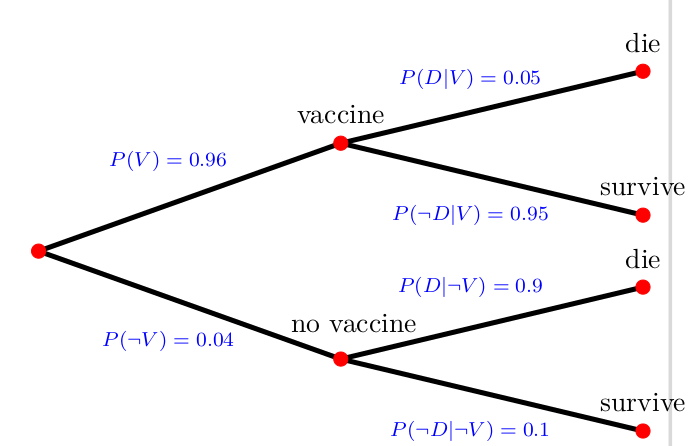
\includegraphics[width=0.5\textwidth,height=\textheight]{fig/diesurvive.png}
\caption{\label{fig:diesurvive} Tree diagramm vaccinated or not}
\end{figure}

The \emph{Tree Diagram} in figure \ref{fig:diesurvive} shows probabililties of people to have a vaccine for some disease. Moreover, it shows the conditional probabilities of people to die given the fact they were vaccinated or not.
\(D\) denotes the event of \emph{die} and \(\neg D\) denotes \emph{not die}, i.e., survive; \(V\) denotes the event of \emph{vaccinated} and \(\neg V\) \emph{not vaccinated}.

\begin{enumerate}
\def\labelenumi{\alph{enumi})}
\tightlist
\item
  Calculate the overall probability to die, \(P(D)\)
\item
  Calculate the probability that a person that has died was vaccinated, \(P(V|D)\).
\end{enumerate}

Please find solution to the exercise \protect\hyperlink{sol:tobevacornot}{in the appendix.}

\begin{quote}
Disclaimer: The case presented here is fictitious. The data given here are purely fictitious and serve only to practice the method.
\end{quote}

\begin{center}\rule{0.5\linewidth}{0.5pt}\end{center}

\end{exercise}

\begin{exercise}
\protect\hypertarget{exr:todieornot}{}\label{exr:todieornot}To die or not to die

You read on Facebook that in the year 2021 about over 80\% of people that died were vaccinated. You are shocked by this high probability that a dead person was vaccinated, \(P(V|D)\). You decide to check this fact. Reading the study to which the Facebook post is referring, you find out that the study only refers to people above the age of 90. Moreover, you find the following \emph{Tree Diargram}. It allows checking the fact as it describes the vaccination rates and the conditional probabilities of people to die given the fact they were vaccinated or not.
In particular, \(D\) denotes the event of \emph{die} and \(\neg D\) denotes \emph{not die}, i.e., survive; \(V\) denotes the event of \emph{vaccinated} and \(\neg V\) \emph{not vaccinated}.
\end{exercise}

\begin{figure}
\centering
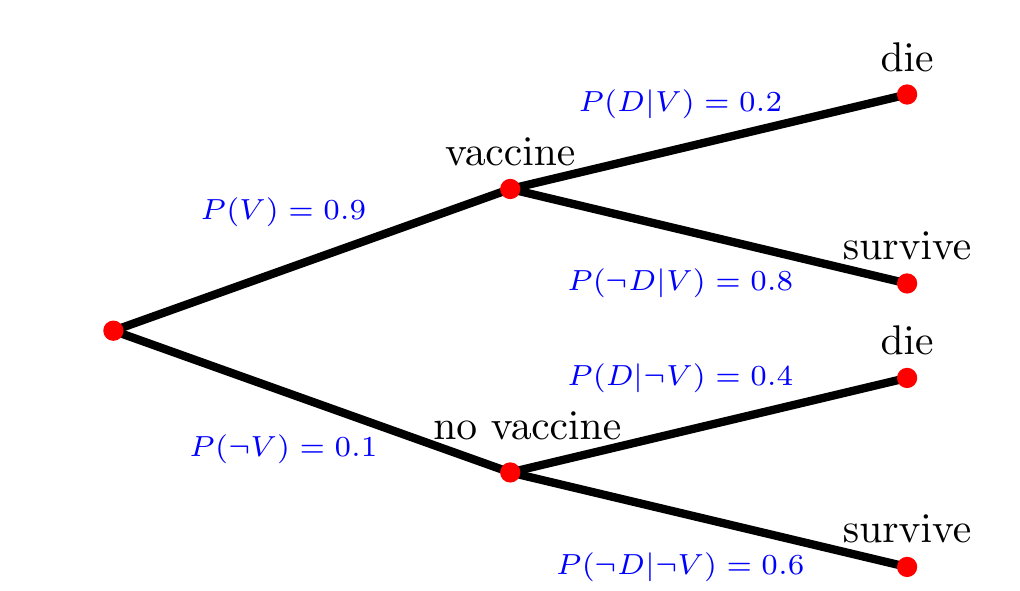
\includegraphics{_main_files/figure-latex/tikz-ex2-1.png}
\caption{\label{fig:tikz-ex2}Tree: To die or not to die}
\end{figure}

\begin{enumerate}
\def\labelenumi{\alph{enumi})}
\tightlist
\item
  Calculate the overall probability to die, \(P(D)\)
\item
  Calculate the probability that a person that has died was vaccinated, \(P(V|D)\).
\item
  Your calculations shows that the fact used in the statement on Facebook is indeed true. Discuss whether this number should have an impact to get vaccinated or not.
\end{enumerate}

\begin{quote}
Disclaimer: The case presented here is fictitious. The data given here are purely fictitious and serve only to practice the method.
\end{quote}

Please find solution to the exercise \protect\hyperlink{sol:todieornot}{in the appendix.}

\begin{center}\rule{0.5\linewidth}{0.5pt}\end{center}

\begin{verbatim}
\end{verbatim}

\begin{exercise}
\protect\hypertarget{exr:falspos}{}\label{exr:falspos}

Corona false positive

Suppose that Corona infects one out of every 1000 people in a population and that the test for it comes back positive in 99\% of all cases if a person has Corona. Moreover, the test also produces some false positive, that is about 2\% of uninfected patients also tested positive.

Now, assume you are tested positive and you want to know the chances of having the disease.
Then, we have two events to work with:

\textbf{A}: you have Corona

\textbf{B}: your test indicates that you have Corona

and we know that
\begin{align*}
    P(A)&=.001  \qquad \rightarrow \text{one out of 1000 has Corona}\\
    P(B|A)&=.99 \qquad \rightarrow \text{probability of a positive test, given infection}\\
    P(B|\neg A)&=.02 \qquad \rightarrow \text{probability of a false positive, given no infection}
\end{align*}

As you don`t like to go into quarantine, you are interested in the probability of having the disease given a positive test, that is \(P(A|B)\)?

\begin{quote}
Disclaimer: The case presented here is fictitious. The data given here are purely fictitious and serve only to practice the method.
\end{quote}

Please find solution to the exercise \protect\hyperlink{sol:falspos}{in the appendix.}

\begin{center}\rule{0.5\linewidth}{0.5pt}\end{center}

\end{exercise}

\hypertarget{cognitive-biases}{%
\section{Cognitive biases in decision making}\label{cognitive-biases}}

In section \ref{bounded-rationality}, we discussed how human beings have limited cognitive abilities to arrive at optimal solutions. Behavioral economics, pioneered by Amos Tversky (1937-1996) and 2002 Nobel Prize winner Daniel Kahnemann (*1934), has identified several biases that explain why and when people fail to act perfectly rationally. In the following sections, we will explore some of the most prominent biases that arise from humans relying on heuristics in decision-making. Specifically, we will describe biases result from the use of availability, representative, and confirmation heuristics and can lead to flawed decision-making and negative outcomes for individuals and organizations. By recognizing and accounting for these biases, we can make better decisions.

\hypertarget{availability-heuristic}{%
\subsection{Availability heuristic}\label{availability-heuristic}}

The \textbf{availability heuristic} refers to our tendency to make judgments or decisions based on information that is easily retrievable from memory. For example, if someone hears a lot of news about a particular stock or investment, they may be more likely to invest in it, even if there are other better investment options available. This bias can also lead individuals to overestimate the frequency of certain events, such as the likelihood of a market crash, based on recent media coverage.

\hypertarget{representative-heuristic}{%
\subsection{Representative heuristic}\label{representative-heuristic}}

The \textbf{representative heuristic} refers to our tendency to make judgments based on how similar something is to a stereotype or preconceived notion. For example, an investor might assume that a company with a flashy website and marketing materials is more successful than a company with a more low-key image, even if the latter is actually more profitable. This bias can also lead to assumptions about the performance of certain investment strategies based on their resemblance to other successful strategies.

\hypertarget{confirmation-heuristic}{%
\subsection{Confirmation heuristic}\label{confirmation-heuristic}}

The \textbf{confirmation heuristic} refers to our tendency to seek out information that confirms our existing beliefs and ignore information that contradicts them. For example, an investor who strongly believes in the potential of a particular investment might only read news and analysis that supports their belief and ignore any information that suggests otherwise. This can lead to a failure to consider potential risks and downsides of an investment.

\begin{exercise}
\protect\hypertarget{exr:bazermanbias}{}\label{exr:bazermanbias}

Twelve cognitive biases

In the textbook of \citet{Bazerman2017Judgement} twelve cognitive biases that are described. Read chapter 2 of the book and summarize the twelve biases in a sentence.

Please find solution to the exercise \protect\hyperlink{sol:bazermanbias}{in the appendix.}

\begin{center}\rule{0.5\linewidth}{0.5pt}\end{center}

\end{exercise}

\hypertarget{decision-making-and-money}{%
\section{Decision making and money}\label{decision-making-and-money}}

\hypertarget{financial-literacy}{%
\subsection{Financial literacy}\label{financial-literacy}}

You are financially literate if you understand and manage personal finances effectively. It involves having a basic understanding of financial concepts, such as budgeting, saving, investing, and managing debt. Financial literacy also includes knowledge of financial products and services, such as bank accounts, credit cards, loans, and insurance.
Being financially literate means having the skills and knowledge to make informed financial decisions, and being able to assess risks and opportunities when it comes to managing money. It is an important life skill that can help individuals achieve their financial goals, build wealth, and avoid financial pitfalls.

Being better-educated was always associated with having more financial knowledge (Figure
1) across the countries we examined,3 yet we also found that education is not enough. That
is, even well-educated people are not necessarily savvy about money.

Unfortunately, financial illiteracy is widespread. While being better-educated is associated with making better financial decisions on average, ``even well-educated people are not necessarily savvy about money'' \citep[p.~3]{Mitchell2015Financial}.

There are various attempts to assess the levels of financial literacy. See \url{https://www.oecd.org/finance/financial-education/measuringfinancialliteracy.htm} for example.

\begin{exercise}
\protect\hypertarget{exr:flmeasure}{}\label{exr:flmeasure}

S\&P Global FinLit Survey

One example of a comprehend way to measure financial literacy stems from the \emph{Standard \& Poor`s Ratings Services Global Financial Literacy Survey} \citep[see][]{Klapper2020Financial}. They ask the following multiple-choice questions:

\begin{enumerate}
\def\labelenumi{\arabic{enumi}.}
\tightlist
\item
  Suppose you have some money. Is it safer to put your money into one business or investment, or to put your money into multiple businesses or investments?

  \begin{enumerate}
  \def\labelenumii{\alph{enumii})}
  \tightlist
  \item
    One business or investment
  \item
    Multiple businesses or investments
  \item
    Don`t know
  \item
    Refused to answer
  \end{enumerate}
\item
  Suppose over the next 10 years the prices of the things you buy double. If your income also doubles, will you be able to buy less than you can buy today, the same as you can buy today, or more than you can buy today?

  \begin{enumerate}
  \def\labelenumii{\alph{enumii})}
  \tightlist
  \item
    Less
  \item
    The same
  \item
    More
  \item
    Don`t know
  \item
    Refused to answer
  \end{enumerate}
\item
  Suppose you need to borrow \$100. Which is the lower amount to pay back: \$105 or \$100 plus 3\%?

  \begin{enumerate}
  \def\labelenumii{\alph{enumii})}
  \tightlist
  \item
    \$105
  \item
    \$100 plus 3\%
  \item
    Don`t know
  \item
    Refused to answer
  \end{enumerate}
\item
  Suppose you put money in the bank for 2 years and the bank agrees to add 15\% per year to your account. Will the bank add more money to your account the second year than it did the first year, or will it add the same amount of money both years?

  \begin{enumerate}
  \def\labelenumii{\alph{enumii})}
  \tightlist
  \item
    More
  \item
    The same
  \item
    Don`t know
  \item
    Refused to answer
  \end{enumerate}
\item
  Suppose you had \$100 in a savings account and the bank adds 10\% per year to the account. How much money would you have in the account after 5 years if you did not remove any money from the account?

  \begin{enumerate}
  \def\labelenumii{\alph{enumii})}
  \tightlist
  \item
    More than \$150
  \item
    Exactly \$150
  \item
    Less than \$150
  \item
    Don`t know
  \item
    Refused to answer
  \end{enumerate}
\end{enumerate}

These questions cover four fields of financial literacy, i.e., risk diversification, inflation and purchasing power, numeracy (simple calculations related to interest rates), and compound interest (interest payments increase exponentially over time). Knowledge in these concepts is important to make good financial decisions and to manage risk.

Try to answer these quesions and compare your performance with the results shown in \citet{Klapper2020Financial}.

Please find solution to the exercise \protect\hyperlink{sol:flmeasure}{in the appendix.}

\begin{center}\rule{0.5\linewidth}{0.5pt}\end{center}

\end{exercise}

\begin{exercise}
\protect\hypertarget{exr:bigthreeiq}{}\label{exr:bigthreeiq}

The \emph{big three} questions

Referring to \citet{Mitchell2015Financial}, only 21.7\% of individuals in Germany with a lower secondary education and 72\% of those with tertiary education can correctly answer all three of the following questions. Try it yourself!

\begin{enumerate}
\def\labelenumi{\arabic{enumi}.}
\tightlist
\item
  Suppose you had \$100 in a savings account and the interest rate was 2\% per year. After 5 years, how much do you think you would have in the account if you left the money to grow?

  \begin{enumerate}
  \def\labelenumii{\alph{enumii})}
  \tightlist
  \item
    More than \$102
  \item
    Exactly \$102
  \item
    Less than \$102
  \item
    Do not know
  \item
    Refuse to answer
  \end{enumerate}
\item
  Imagine that the interest rate on your savings account was 1\% per year and inflation was 2\% per year. After 1 year, how much would you be able to buy with the money in this account?

  \begin{enumerate}
  \def\labelenumii{\alph{enumii})}
  \tightlist
  \item
    More than today
  \item
    Exactly the same
  \item
    Less than today
  \item
    Do not know
  \item
    Refuse to answer
  \end{enumerate}
\item
  Please tell me whether this statement is true or false: \emph{``Buying a single company's stock usually provides a safer return than a stock mutual fund.''}

  \begin{enumerate}
  \def\labelenumii{\alph{enumii})}
  \tightlist
  \item
    True
  \item
    False
  \item
    Do not know
  \item
    Refuse to answer
  \end{enumerate}
\end{enumerate}

These three questions are designed to measure
\citet{Lusardi2014Economic} reports that in many countries the financial illiteracy is considerably high as the following table shows:

\begin{longtable}[]{@{}lcc@{}}
\caption{Financial literacy around the World}\tabularnewline
\toprule\noalign{}
& \% all correct & \% none correct \\
\midrule\noalign{}
\endfirsthead
\toprule\noalign{}
& \% all correct & \% none correct \\
\midrule\noalign{}
\endhead
\bottomrule\noalign{}
\endlastfoot
Germany & 57 & 10 \\
Netherlands & 46 & 11 \\
United States & 35 & 10 \\
Italy & 28 & 20 \\
Sweden & 27 & 11 \\
Japan & 27 & 17 \\
New Zealand & 27 & 4 \\
Russia & 3 & 28 \\
\end{longtable}

Please find solution to the exercise \protect\hyperlink{sol:bigthreeiq}{in the appendix.}

\begin{center}\rule{0.5\linewidth}{0.5pt}\end{center}

\end{exercise}

\hypertarget{common-investment-mistakes}{%
\subsection{Common investment mistakes}\label{common-investment-mistakes}}

Investing can be a daunting task, but avoiding some common investment mistakes can help set you on the right path to financial success.
The following list list shows according to \citet{Stammers2016Tips} the \emph{Top 20 common investment mistakes} without the explanations provided in the paper:

\begin{itemize}
\tightlist
\item
  Expecting too much or using someone else's expectations
\item
  Not having clear investment goals
\item
  Failing to diversify enough
\item
  Focusing on the wrong kind of performance
\item
  Buying high and selling low
\item
  Trading too much and too often
\item
  Paying too much in fees and commissions
\item
  Focusing too much on taxes
\item
  Not reviewing investments regularly
\item
  Taking too much, too little, or the wrong risk
\item
  Not knowing the true performance of your investments
\item
  Reacting to the media
\item
  Chasing yield
\item
  Trying to be a market timing genius
\item
  Not doing due diligence
\item
  Working with the wrong adviser
\item
  Letting emotions get in the way
\item
  Forgetting about inflation
\item
  Neglecting to start or continue
\item
  Not controlling what you can
\end{itemize}

\begin{exercise}
\protect\hypertarget{exr:commistakes}{}\label{exr:commistakes}

Common investment mistakes

Read the paper and summarize the 20 mistakes.

Please find solution to the exercise \protect\hyperlink{sol:commistakes}{in the appendix.}

\begin{center}\rule{0.5\linewidth}{0.5pt}\end{center}

\end{exercise}

\hypertarget{simple-financial-mathematics}{%
\subsection{Simple financial mathematics}\label{simple-financial-mathematics}}

I discuss financial mathematics in the following chapter just briefly. If you want to gather a deeper understanding, I recommend the open textbook of \citet{Dahlquist2022Principles} or the respective chapters of \citet{Wilkinson2022Managerial}.

\hypertarget{simple-interest}{%
\subsubsection{Simple Interest}\label{simple-interest}}

Suppose \(r\) denotes annual interest rates, \(P\) denotes the initial deposit which earns the interest, \(A\) denotes the value of the deposit at the end of an investment. Then, the relationship of these for a single year is

\[
A=P+Pr=P(1+r)
\]

and for many years, \(t\), it is

\[
A=P(1+rt)
\]

which is the simple interest formula. It gives the amount due when the annual interests does not become part of the deposit \(P\).

\hypertarget{compound-interest}{%
\subsubsection{Compound interest}\label{compound-interest}}

If the annual interest, \(P(1+r)\), is added to \(P\), we need a formula that takes this into account, and for two periods this is

\[
A=P\cdot  [(1+r)\cdot(1+r)]=P(1+r)^2
\]

and for t periods

\[
A=P(1+r)^t.
\]

Compound interest is the addition of interest to the principal sum of a loan or deposit, or in other words, interest on principal plus interest. It is the result of reinvesting interest, or adding it to the loaned capital rather than paying it out, or requiring payment from borrower, so that interest in the next period is then earned on the principal sum plus previously accumulated interest.

\[
A=P\left(1+\frac{r}{n}\right)^{nt}
\]

\hypertarget{example}{%
\paragraph*{Example}\label{example}}
\addcontentsline{toc}{paragraph}{Example}

Suppose a principal amount of \$1,500 is deposited in a bank paying an annual interest rate of 4.3\%, compounded quarterly. Then the balance after 6 years is found by using the formula above, with \(P = 1500\), \(r = 0.043\) (4.3\%), \(n = 4\), and \(t = 6\):

\[
A=1500\times\left(1+\frac{0.043}{4}\right)^{4\times 6}\approx 1938.84
\]

So the amount \(A\) after 6 years is approximately \$1,938.84.

Subtracting the original principal from this amount gives the amount of interest received: \(1938.84-1500=438.84\)

\hypertarget{continuously-compounded-interest}{%
\subsubsection{Continuously compounded interest}\label{continuously-compounded-interest}}

As \(n\), the number of compounding periods per year, increases without limit, the case is known as continuous compounding, in which case the effective annual rate approaches an upper limit of \(e^r- 1\), where \(e\) is a mathematical constant that is the base of the natural logarithm.

Continuous compounding can be thought of as making the compounding period infinitesimally small, achieved by taking the limit as \(n\) goes to infinity. The amount after \(t\) periods of continuous compounding can be expressed in terms of the initial amount \(P\) as

\[
A=Pe^{rt}
\]

\hypertarget{present-value}{%
\subsubsection{Present value}\label{present-value}}

The present is the value of an expected income stream determined as of the date of valuation. The present value is usually less than the future value because money has interest-earning potential, a characteristic referred to as the time value of money, except during times of zero- or negative interest rates, when the present value will be equal or more than the future value. Time value can be described with the simplified phrase, ``A dollar today is worth more than a dollar tomorrow'`. Here, 'worth more' means that its value is greater than tomorrow. A dollar today is worth more than a dollar tomorrow because the dollar can be invested and earn a day's worth of interest, making the total accumulate to a value more than a dollar by tomorrow.

\[
P=Ae^{-rt}
\]

\hypertarget{net-present-value-and-internal-rate-of-return}{%
\subsection{Net present value and internal rate of return}\label{net-present-value-and-internal-rate-of-return}}

When making decisions about financial products such as investments or loans, it is important to consider their long-term impact on your finances. \emph{Net Present Value} (NPV) and \emph{Internal Rate of Return} (IRR) are two key indicators that can help guide decision making and determine whether a financial product is a good investment.

Net Present Value (NPV) is the difference between the present value of all cash inflows and the present value of all cash outflows over a given time period. The formula to calculate NPV is:

\[ NPV = \sum_{n=1}^{N} \frac{C_n}{(1+r)^n} - C_0 \]

where \(C_n\) denotes net cash inflow during the period \(n\), \(r\) the discount rate, or the cost of capital, \(n\) the number of periods, and \(C_0\) the initial investment.

In other words, NPV helps determine the current value of future cash flows, adjusted for the time value of money. A positive NPV indicates that an investment is expected to generate a return greater than the cost of capital, while a negative NPV suggests that the investment is likely to result in a loss.

Internal Rate of Return (IRR), on the other hand, is the discount rate that makes the NPV of all cash inflows equal to the NPV of all cash outflows. The formula to calculate IRR is:

\[ 0 = \sum_{n=0}^{N} \frac{C_n}{(1+IRR)^n}  \]

where \(C_n\) denotes the net cash inflow during the period \(n\), \(IRR\) the internal rate of return, \(n\) the number of periods, and \(C_0\) the initial investment.

IRR can be thought of as the rate of return an investment generates over time, taking into account the time value of money. When comparing different investment opportunities, a higher IRR generally indicates a more profitable investment.

Both NPV and IRR are important tools to help individuals make informed decisions about financial products. By comparing the NPV and IRR of different investment options, individuals can determine which investments are likely to generate the greatest returns over time, and which products may not be worth the initial investment.

It is worth noting that while NPV and IRR are useful indicators for decision making, they are not the only factors to consider. Individuals should also consider other important factors such as risk, liquidity, and diversification when evaluating different financial products. By taking a holistic approach and considering all relevant factors, individuals can make informed decisions that are best suited to their financial goals and circumstances.

\begin{exercise}
\protect\hypertarget{exr:invcase}{}\label{exr:invcase}

Investment case

You deposit 1,000 euros today into a savings account with an annual interest rate of 5\% for 2 years. What is the balance after 2 years with annual, semi-annual (4 interest payments per year), and continuous compounding?

Please find solution to the exercise \protect\hyperlink{sol:invcase}{in the appendix.}

\begin{center}\rule{0.5\linewidth}{0.5pt}\end{center}

\end{exercise}

\begin{exercise}
\protect\hypertarget{exr:presentvalueC}{}\label{exr:presentvalueC}

Present value

You want to have 100,000 in 10 years, and you can save money with an interest rate of 5\% p.a. How much do you need to invest today for annual, semi-annual (4 interest periods), and continuous compounding to achieve your goal?

Please find solution to the exercise \protect\hyperlink{sol:presentvalueC}{in the appendix.}

\begin{center}\rule{0.5\linewidth}{0.5pt}\end{center}

\end{exercise}

\begin{exercise}
\protect\hypertarget{exr:invaorb}{}\label{exr:invaorb}

Invest in A or B

You are considering investing in project A or B.

\textbf{Project A:} It costs 50,000 today and is expected to generate cash flows of 20,000 per year for the next 5 years. You have a required rate of return of 8\%.

\textbf{Project B:} It costs 50,000 today and you get 100,000 back in 5 years.

Calculate the value of your invest after five years. Which investment is the better one?

Please find solution to the exercise \protect\hyperlink{sol:invaorb}{in the appendix.}

\begin{center}\rule{0.5\linewidth}{0.5pt}\end{center}

\end{exercise}

\begin{exercise}
\protect\hypertarget{exr:netpresentvalue}{}\label{exr:netpresentvalue}

Net present value

You are considering investing in project A or B.

\textbf{Project A:} It costs 50,000 today and is expected to generate cash flows of 20,000 per year for the next 5 years. You have a required rate of return of 8\%.

\textbf{Project B:} It costs 50,000 today and you get 100,000 back in 5 years.

Calculate the net present value of both projects and decide where to invest.

Please find solution to the exercise \protect\hyperlink{sol:netpresentvalue}{in the appendix.}

\begin{center}\rule{0.5\linewidth}{0.5pt}\end{center}

\end{exercise}

\begin{exercise}
\protect\hypertarget{exr:irr}{}\label{exr:irr}

Internal rate of return

You are considering investing in project A or B.

\textbf{Project A:} It costs 50,000 today and is expected to generate cash flows of 20,000 per year for the next 5 years. You have a required rate of return of 8\%.

\textbf{Project B:} It costs 50,000 today and you get 100,000 back in 5 years.

Calculate the internal rate of return of both projects with the help of a software package such as \emph{Excel} or \emph{Libre Calc} and decide where to invest.

Please find solution to the exercise \protect\hyperlink{sol:irr}{in the appendix.}

\begin{center}\rule{0.5\linewidth}{0.5pt}\end{center}

\end{exercise}

\begin{exercise}
\protect\hypertarget{exr:rule70}{}\label{exr:rule70}

Rule of 70

The \emph{Rule of 70} is often used to approximate the time required for a growing series to double. To understand this rule calculate how many periods it takes to double your money when it growth at a constant rate of 1\% each period.

Please find solution to the exercise \protect\hyperlink{sol:rule70}{in the appendix.}

\begin{center}\rule{0.5\linewidth}{0.5pt}\end{center}

\end{exercise}

\hypertarget{a-note-on-growth-rates-and-the-logarithm}{%
\subsection{A note on growth rates and the logarithm}\label{a-note-on-growth-rates-and-the-logarithm}}

Most data are recorded for discrete periods of time (e.g., quarters, years). Consequently, it is often useful to model economic dynamics in discrete periods of time. A good linear approximation to a growth rate from time \(t=0\) to \(t=1\) in \(x\) is \(\ln x_0 - \ln x_1\):

\[
\frac{x_1 - x_0}{x_0} \approx \ln x_1 - \ln x_0
\]

Let us prove that with some numbers of per capita real GDP for the US and Japan in 1950 and 1989:

\begin{center}
    \begin{tabular}{ccc}\toprule
        1950 & 1950 & 1989 \\ \midrule
        US & 8611 & 18317 \\ 
        Japan & 1563 & 15101 \\ \bottomrule
    \end{tabular} 
\end{center}

What are the annual average growth rates over this period for the US and Japan? Here is one way to answer this question:

\[
Y_{1989} = (1 + g)^{39} \cdot Y_{1950}
\]

Consequently, \(g\) can be calculated as:

\[
(1 + g) = \left(\frac{Y_{1989}}{Y_{1950}}\right)^{\frac{1}{39}}
\]

Yielding \(g = 0.0195\) for the US and \(g = 0.0597\) for Japan. The US grew at an average growth rate of about 2\% annually over the period, while Japan grew at about 6\% annually.

The following method gives a close approximation to the answer above and will be useful in other contexts. A useful approximation is that for any small number \(x\): \(\ln (1 + x) \approx x\)

Now, we can take the natural log of both sides of:

\[
\frac{Y_{1989}}{Y_{1950}} = (1 + g)^{39}
\]

to get:

\[
\ln (Y_{1989}) - \ln (Y_{1950}) = 39 \cdot \ln (1 + g)
\]

which rearranges to:

\[
\ln (1 + g) = \frac{\ln (Y_{1989}) - \ln (Y_{1950})}{39}
\]

and using our approximation:

\[
g \approx \frac{\ln (Y_{1989}) - \ln (Y_{1950})}{39}
\]

In other words, log growth rates are good approximations for percentage growth rates. Calculating log growth rates for the data above, we get \(g \approx 0.0194\) for the US and \(g \approx 0.0582\) for Japan. The approximation is close for both.

\hypertarget{plotting-growth-using-the-logarithm}{%
\subsubsection*{Plotting growth using the logarithm}\label{plotting-growth-using-the-logarithm}}
\addcontentsline{toc}{subsubsection}{Plotting growth using the logarithm}

Recall that, with a constant growth rate \(g\) and starting from time 0, output in time \(t\) is:

\[Y_t = (1 + g)^t \cdot Y_0\]

Taking natural logs of both sides, we have:

\[\ln Y_t = \ln Y_0 + t \cdot \ln (1 + g)\]

We see that log output is linear in time. Thus, if the growth rate is constant, a plot of log output against time will yield a straight line. Consequently, plotting log output against time is a quick way to \textbf{eyeball} whether growth rates have changed over time.

\begin{figure}
\centering
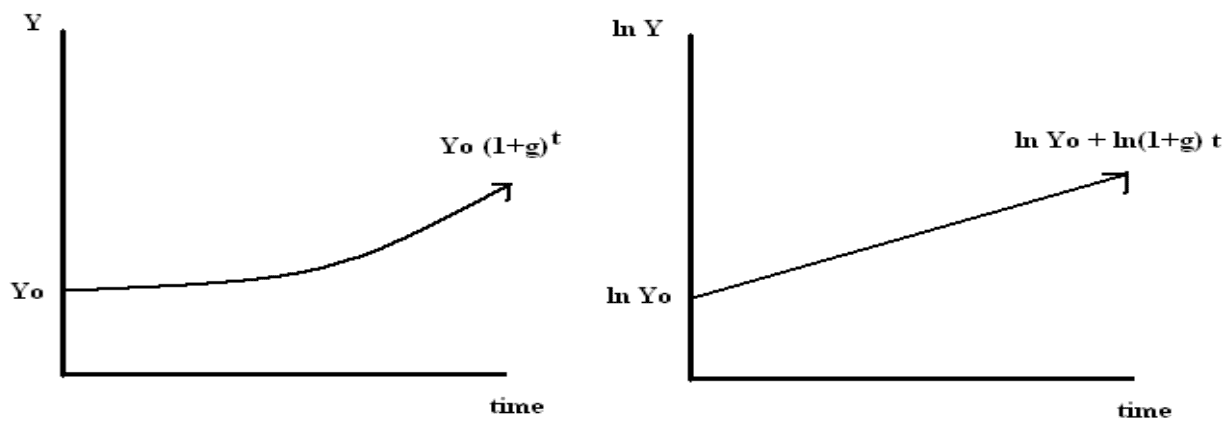
\includegraphics[width=0.5\textwidth,height=\textheight]{fig/logplot.png}
\caption{\label{fig:logplot} Log Plot}
\end{figure}

In figure \ref{fig:logplot} and \ref{fig:loginscale} you see a semi-logarithmic plot that has one axis on a logarithmic scale and the other on a linear scale. It is useful for data with exponential relationships, where one variable covers a large range of values, or to zoom in and visualize that what seems to be a straight line in the beginning is, in fact, the slow start of a logarithmic curve that is about to spike, and changes are much bigger than thought initially.

\begin{figure}
\centering
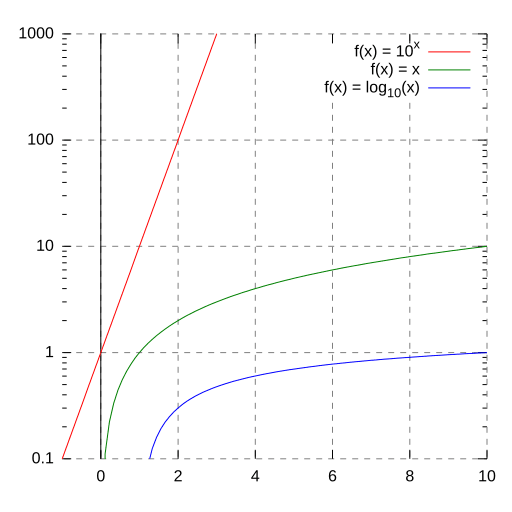
\includegraphics[width=0.5\textwidth,height=\textheight]{fig/LogLinScale.png}
\caption{\label{fig:loginscale} Log-Lin Scale}
\end{figure}

\begin{center}\rule{0.5\linewidth}{0.5pt}\end{center}

\begin{exercise}
\protect\hypertarget{exr:invovertime}{}\label{exr:invovertime}

Investments over time
Describe the formulas to describe the growth process of an investment over time when time is discrete and when time is continuous.

Please find solution to the exercise \protect\hyperlink{sol:invovertime}{in the appendix.}

\begin{center}\rule{0.5\linewidth}{0.5pt}\end{center}

\end{exercise}

\begin{exercise}
\protect\hypertarget{exr:expovertime}{}\label{exr:expovertime}

Exponential growth

Sketch a timeline for each of the following series:

\begin{itemize}
\tightlist
\item
  \(a_t=a_{t-1}+g\)
\item
  \(\ln(a_t)\)
\item
  \(b_t=b_{t-1}\cdot (1+g)\)
\item
  \(\ln b_t\)
\end{itemize}

Please find solution to the exercise \protect\hyperlink{sol:expovertime}{in the appendix.}

\begin{center}\rule{0.5\linewidth}{0.5pt}\end{center}

\end{exercise}

\begin{exercise}
\protect\hypertarget{exr:Covidcases}{}\label{exr:Covidcases}

COVID and how to plot it

I downloaded the complete \textbf{Our World in Data COVID-19} dataset from \href{https://ourworldindata.org/coronavirus/country/germany}{ourworldindata.org}. I created some graphs which I will show you below. Can you discuss the scaling and how to interpret them? What is your opinion on these graphs? Are some of them a bit misleading (at least if you don't look twice)?

\begin{figure}
\centering
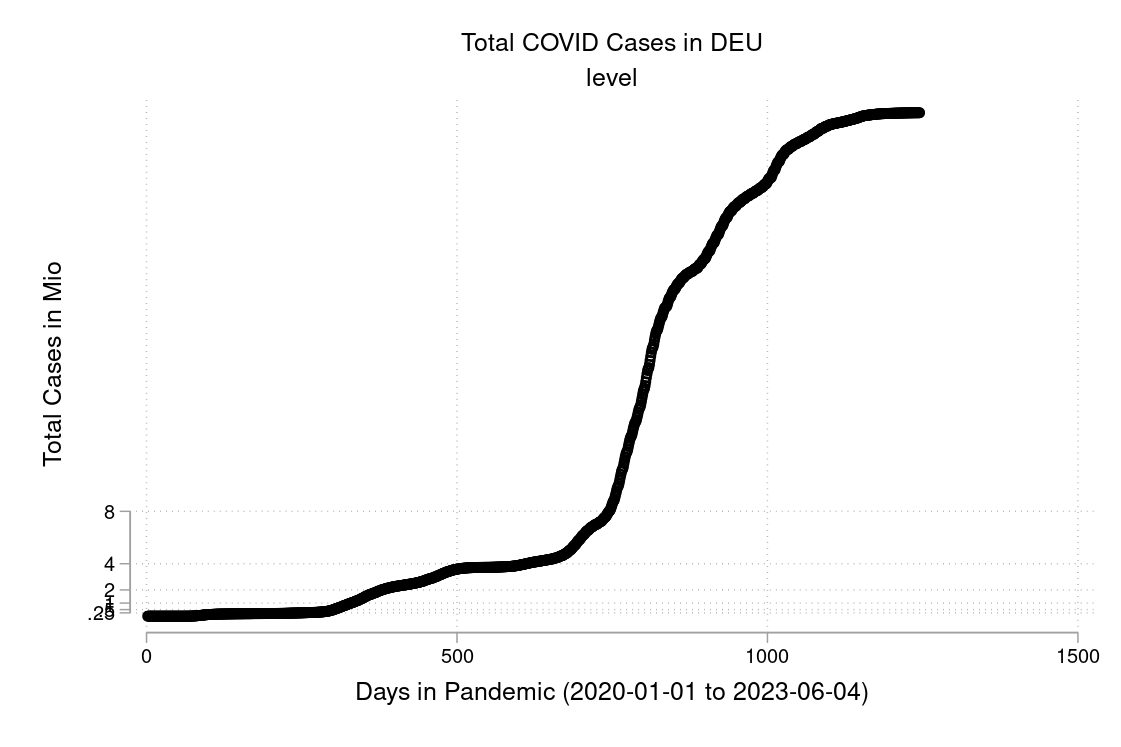
\includegraphics[width=0.5\textwidth,height=\textheight]{fig/total.png}
\caption{Total Cases}
\end{figure}

\begin{figure}
\centering
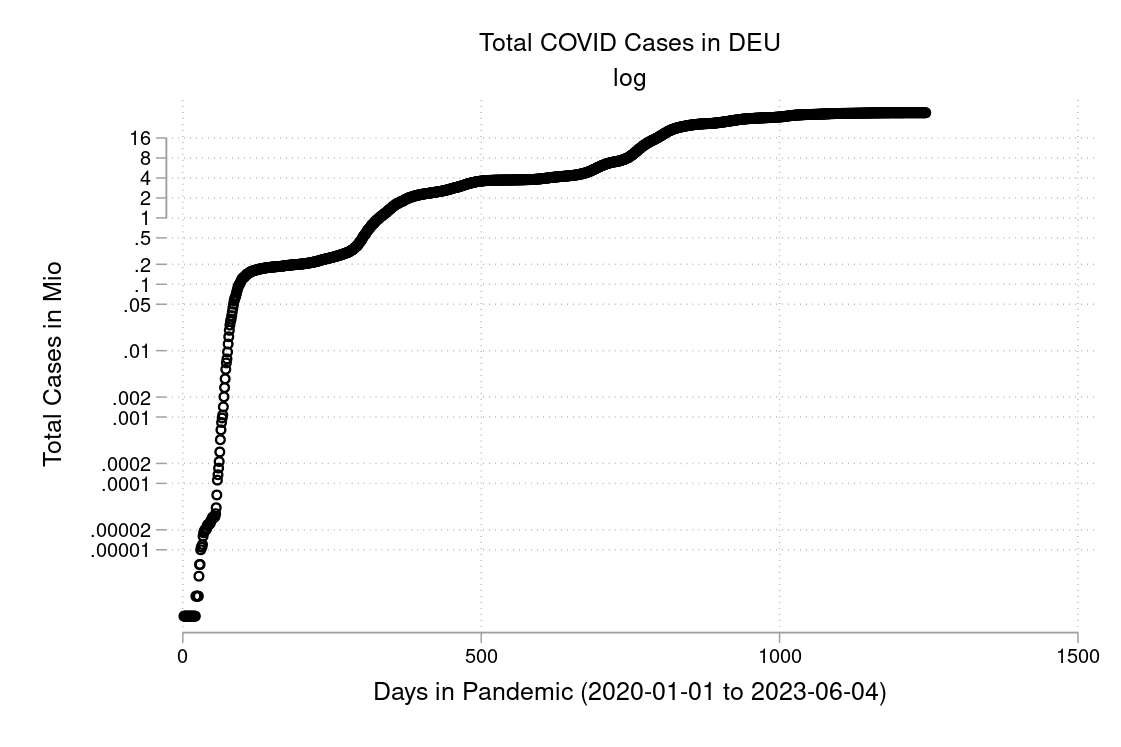
\includegraphics[width=0.5\textwidth,height=\textheight]{fig/total2.png}
\caption{Total Cases 2}
\end{figure}

\begin{figure}
\centering
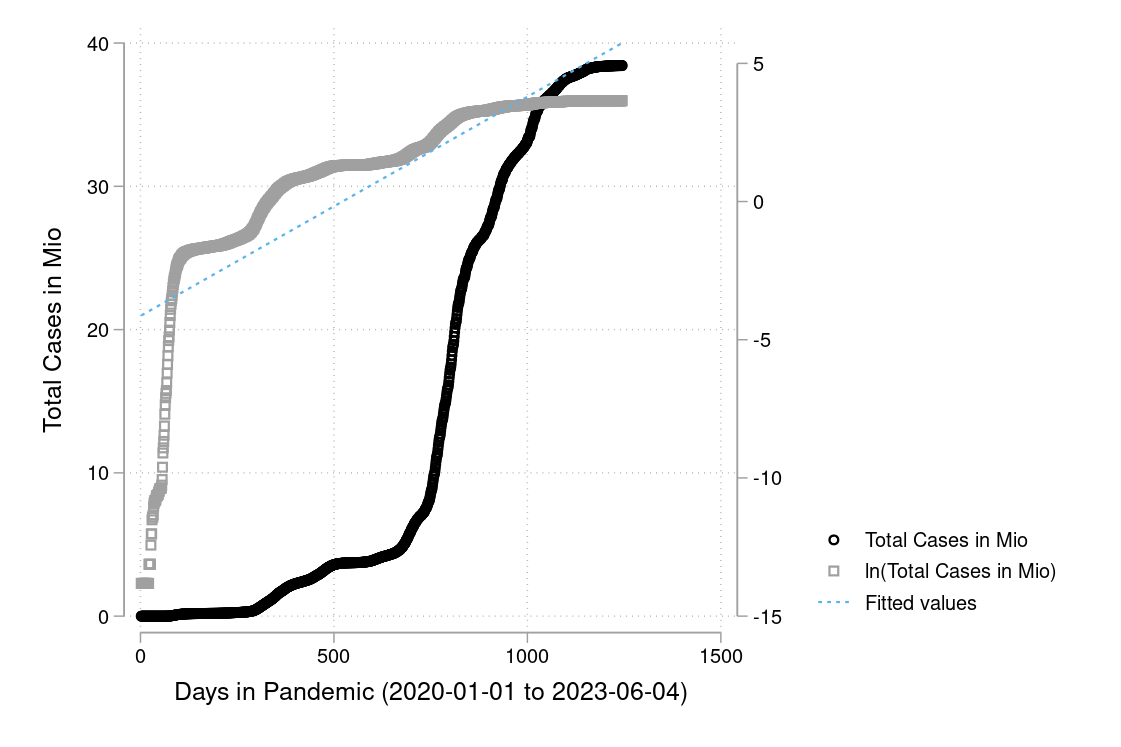
\includegraphics[width=0.5\textwidth,height=\textheight]{fig/total3.png}
\caption{Total Cases 3}
\end{figure}

\begin{figure}
\centering
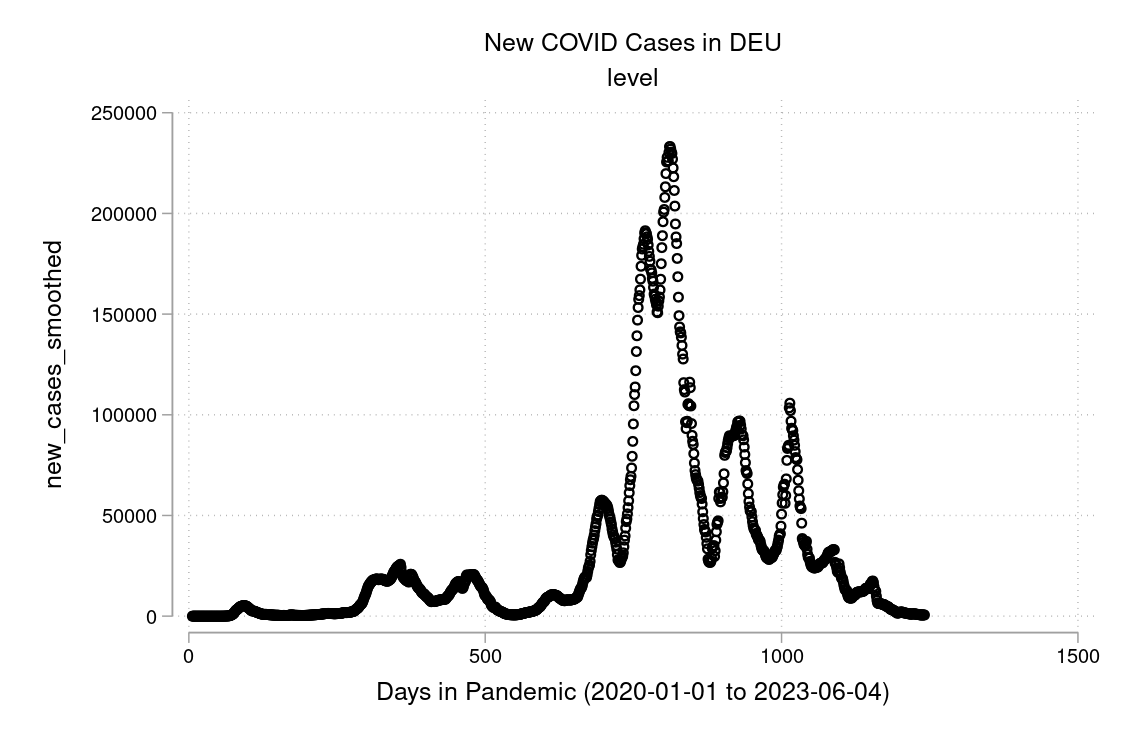
\includegraphics[width=0.5\textwidth,height=\textheight]{fig/new.png}
\caption{New Cases}
\end{figure}

\begin{figure}
\centering
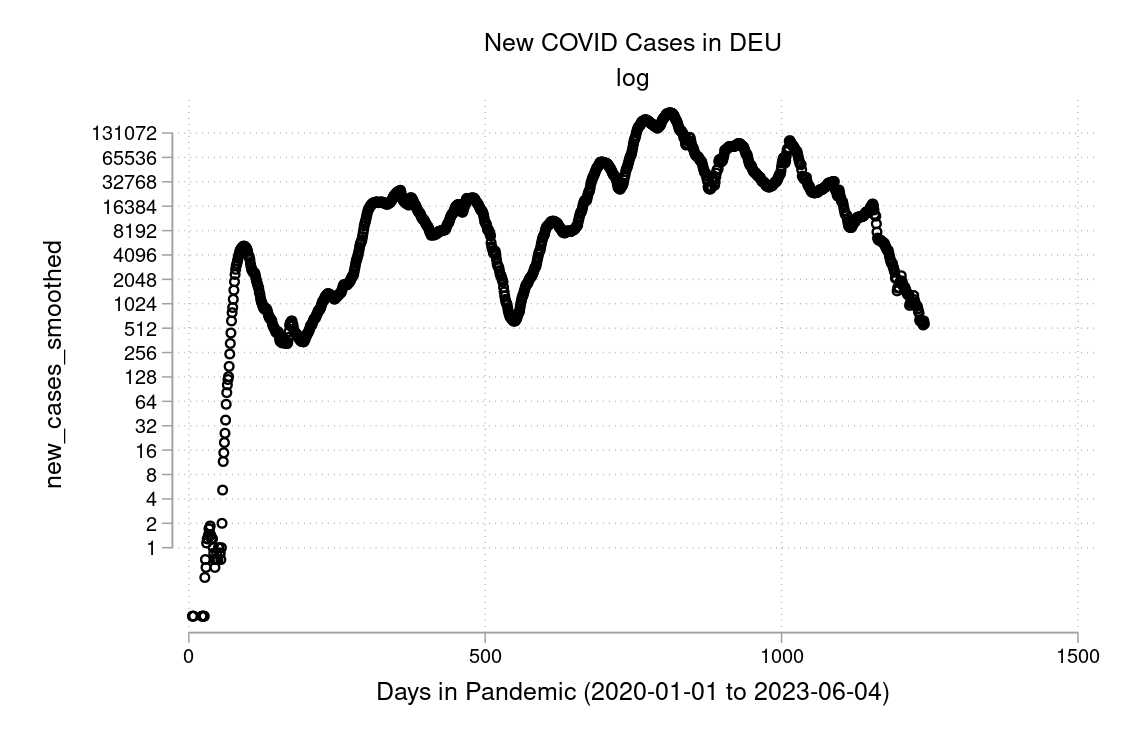
\includegraphics[width=0.5\textwidth,height=\textheight]{fig/new2.png}
\caption{New Cases 2}
\end{figure}

\begin{figure}
\centering
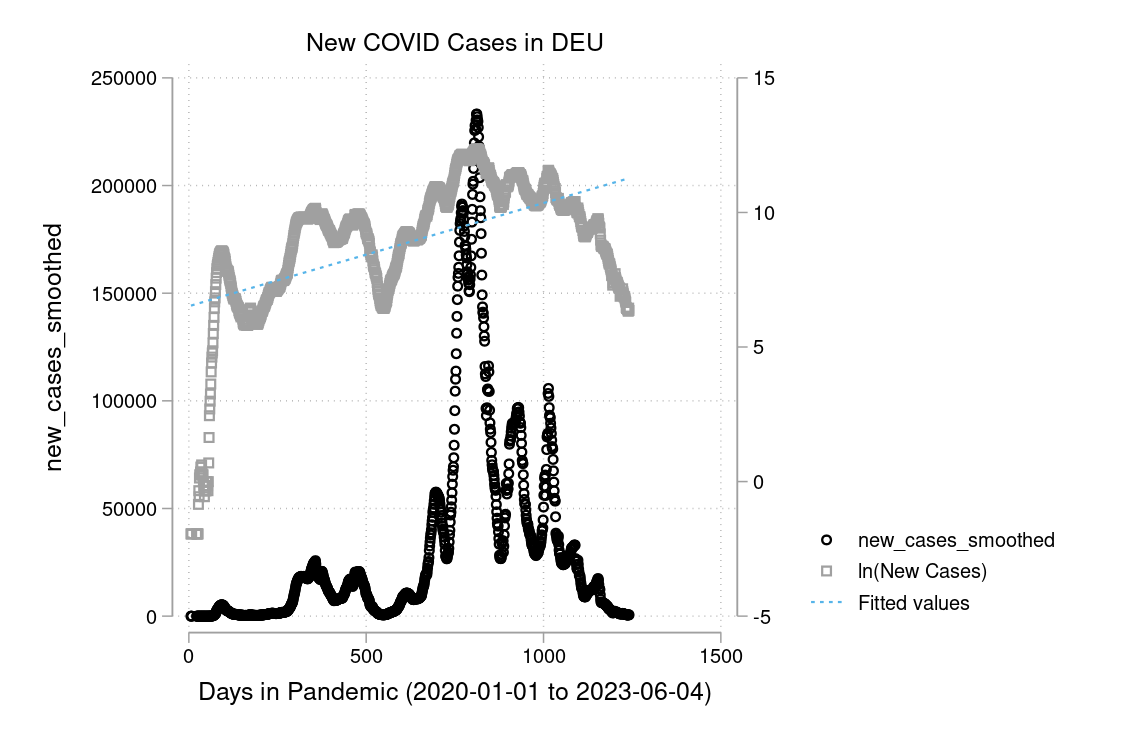
\includegraphics[width=0.5\textwidth,height=\textheight]{fig/new3.png}
\caption{New Cases 3}
\end{figure}

\begin{center}\rule{0.5\linewidth}{0.5pt}\end{center}

\end{exercise}

\hypertarget{managerial-microeconomics}{%
\chapter{Managerial microeconomics}\label{managerial-microeconomics}}

\hypertarget{consumption-and-production-choices}{%
\section{Consumption and production choices}\label{consumption-and-production-choices}}

In microeconomics, utility maximization (in its simplest form when having just two goods) involves selecting a combination of two goods that satisfies two essential conditions, see figure \ref{fig:optimalconsumption}:

\begin{enumerate}
\def\labelenumi{\arabic{enumi}.}
\tightlist
\item
  The chosen point of utility maximization must fall within the attainable region defined by the Production Possibility Frontier (PPF) or be affordable within the constraints of a given budget.
\item
  The selected point of utility maximization must lie on the highest indifference curve that is consistent with the first condition.
\end{enumerate}

\begin{figure}
\centering
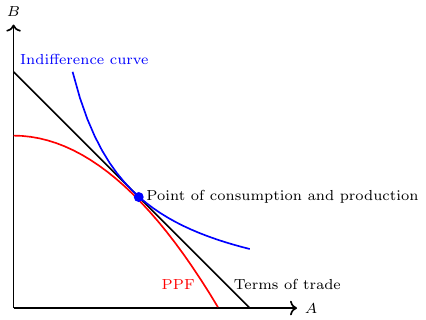
\includegraphics[width=0.5\textwidth,height=\textheight]{fig/optimalconsumption.png}
\caption{\label{fig:optimalconsumption} Optimal consumption}
\end{figure}

These conditions ensure that the consumer selects the optimal bundle of goods that maximizes their utility while taking into account the constraints imposed by production capabilities or budget limitations.

By analyzing production possibilities and individual preferences, economists gain insights into how consumers make choices, allocate resources, and achieve utility maximization. Understanding these concepts helps economists explore the trade-offs and decision-making processes that influence consumer behavior and shape market dynamics.

If you are not familiar with the basic principles of the production possibility frontier curve, indifference curves, and budget constraints, I recommend referring to section \ref{micro-pre} of the appendix for a comprehensive overview. This section provides a detailed explanation and exploration of these concepts.

\hypertarget{the-role-of-income-and-budget}{%
\subsection{The role of income and budget}\label{the-role-of-income-and-budget}}

If income increases the budget constraint curve shifts outwards (to the right) as shown in figure \ref{fig:incomechange}.

\begin{figure}
\centering
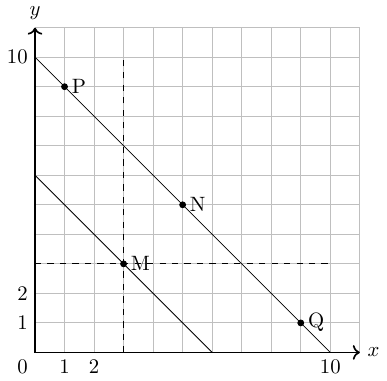
\includegraphics[width=0.5\textwidth,height=\textheight]{fig/incomechange.png}
\caption{\label{fig:incomechange} Impact of income change on consumption}
\end{figure}

The utility-maximizing choice on the original budget constraint is M. The dashed horizontal and vertical lines extending through point M allow you to see at a glance whether the quantity consumed of goods on the new budget constraint is higher or lower than on the original budget constraint. On the new budget constraint, a choice like N will be made if both goods are \emph{normal goods}. If good \(x\) is an \emph{inferior good}, a choice like P will be made. If good \(y\) is an \emph{inferior good}, a choice like Q will be made.

\hypertarget{the-role-of-prices}{%
\subsection{The role of prices}\label{the-role-of-prices}}

If price of one good increases then the budget constraint curve. When the price rises, the budget constraint shifts in to the left for that good.

\begin{figure}
\centering
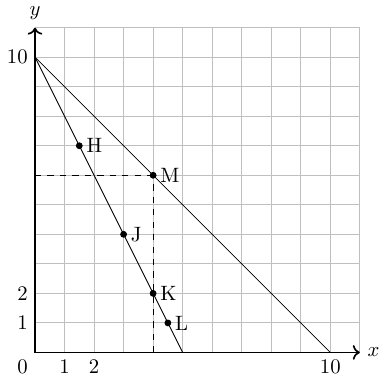
\includegraphics[width=0.5\textwidth,height=\textheight]{fig/pricechange.png}
\caption{\label{fig:pricechange} Impact of price change on consumption}
\end{figure}

The dashed lines make it possible to see at a glance whether the new consumption choice involves less of both goods, or less of one good and more of the other. The new possible choices would be good \(x\)'s and more good \(y\)'s, like point H, or less of both goods, as at point J. Choice K would mean that the higher price of good \(x\) led to exactly the same quantity of good \(x\) being consumed, but fewer of good \(y\). Choices like L are theoretically possible (if good \(x\) are giffen goods) but highly unlikely in the real world, because they would mean that a higher price for goods \(x\) means a greater quantity consumed of good \(x\).

\hypertarget{substitution-and-income-effect}{%
\subsection{Substitution and income effect}\label{substitution-and-income-effect}}

When prices increase, individuals typically respond by reducing their consumption of the product with the higher price. This reaction is driven by two factors, both of which can occur simultaneously.

\begin{figure}
\centering
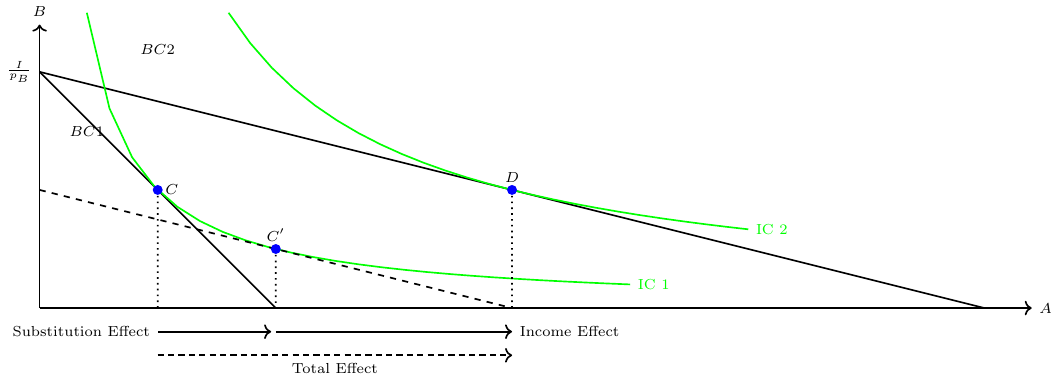
\includegraphics[width=1\textwidth,height=\textheight]{fig/hicksdecomp.png}
\caption{\label{fig:hicksdecomp} Impact of income change on consumption}
\end{figure}

The \emph{substitution effect} occurs when a price change incentivizes consumers to consume less of a good with a relatively higher price and more of a good with a relatively lower price.

The \emph{income effect} stems from the fact that a higher price effectively reduces the purchasing power of income (even if actual income remains the same). This reduction in purchasing power leads to a decrease in the consumption of the good, particularly when the good is considered normal.

Figure \ref{fig:hicksdecomp} illustrates the Hicksian decomposition for a price reduction of good \(A\), which affects the consumption of goods \(A\) and \(B\), shifting the consumption point from \(C\) to \(D\). The point \(C'\) represents the hypothetical consumption point resulting from a rotated budget constraint that reflects the new price relationship.

\begin{exercise}
\protect\hypertarget{exr:twopointsofconsumption}{}\label{exr:twopointsofconsumption}The graphical foundations of demand curves

A shift in the budget constraint means that when individuals are seeking their highest utility, the quantity that is demanded of that good will change. In this way, the logical foundations of demand curves---which show a connection between prices and quantity demanded---are based on the underlying idea of individuals seeking utility.

In Figure \ref{fig:tpoc}, two points of consumption are displayed, illustrating the optimal choices made by customers when faced with prices \(p_x^1>p_x^2\). The objective of this exercise is to graphically derive the demand function for good \(x\). To accomplish this, please provide a second two-dimensional plot below the existing graph, with the price of good \(x\), \(p_x\), represented on the y-axis.
\end{exercise}

\begin{figure}
\centering
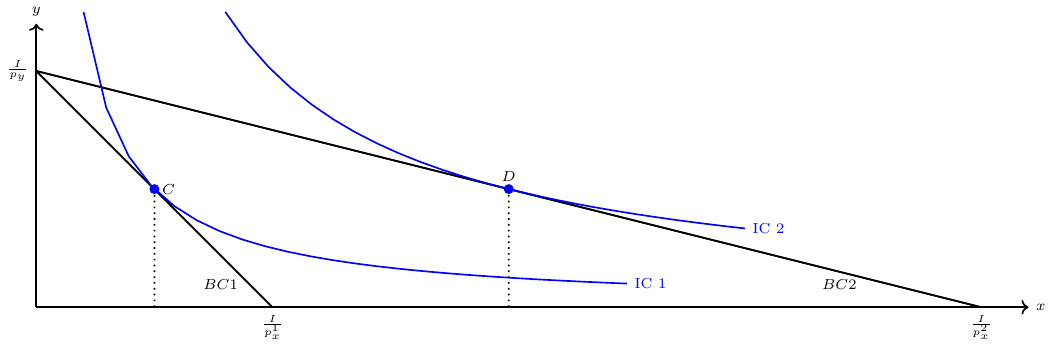
\includegraphics[width=1\textwidth,height=\textheight]{fig/twopointsofconsumption.png}
\caption{\label{fig:tpoc} Graphical derivation of the demand function}
\end{figure}

\begin{exercise}
\protect\hypertarget{exr:derofdemand}{}\label{exr:derofdemand}Derivation of demand function using the Lagranian multiplier

A representative consumer has on average the following utility function:
\(U=x y,\) and faces a budget constraint of \(B=P_{x} x+P_{y} y,\) where \(B, P_{x}\)
and \(P_{y}\) are the budget and prices, which are given. Solve the following choice problem:

Maximize \(U=x y\) s.t. \(B=P_{x} x+P_{y} y\).

Please find solution to the exercise \protect\hyperlink{sol:derofdemand}{in the appendix.}
\end{exercise}

\begin{exercise}
\protect\hypertarget{exr:cdanddemand}{}\label{exr:cdanddemand}

Cobb-Douglas and demand

A consumer who has a Cobb-Douglas utility function \(u(x, y)=A x^{\alpha} y^{\beta}\)
faces the budget constraint \(p x+q y=I\), where \(A, \alpha, \beta, p,\) and \(q\) are
positive constants.
Solve the problem:

\[
\begin{array}{lll}
\max A x^{\alpha} y^{\beta} & \text { subject to } & p x+q y=I
\end{array}
\]

Please find solution to the exercise \protect\hyperlink{sol:cdanddemand}{in the appendix.}

\hypertarget{consumption-production-and-terms-of-trade}{%
\subsection{Consumption, production, and terms of trade}\label{consumption-production-and-terms-of-trade}}

Market prices in a closed economy:
The price relation of two goods, the so-called terms of trade, is determined by the slope of the Production Possibility Frontier (PPF) at the point where it is tangent to the indifference curve. This relationship highlights the trade-off between the two goods and their relative scarcity within a closed economy.

Utility maximizing production:
The production point that maximizes utility is where the PPF is tangent to the price relation, i.e.~the \emph{terms of trade}. This principle applies not only in a closed economy (autarky) but also under free trade (open economy). It implies that producers should allocate resources in a way that balances the trade-off between producing more of one good at the expense of another, while considering consumer preferences. Figure \ref{fig:optimalconsumption} depicts this.

\begin{center}\rule{0.5\linewidth}{0.5pt}\end{center}

\end{exercise}

\begin{exercise}
\protect\hypertarget{exr:Uic}{}\label{exr:Uic}Understanding indifference curves and budget constraints

\begin{enumerate}
\def\labelenumi{\alph{enumi})}
\tightlist
\item
  Which indifference curve in the figure on the right represents the highest utility level? Explain your decision.
\item
  Suppose two goods are perfect substitutes\footnote{Two goods are substitutes if they can be used for the same purpose or provide the same utility to the consumer}. Draw the indifference curves for perfect substitutes.
\item
  Suppose two goods are perfect complements\footnote{Two goods are complements if they go well together and the demand for one good is related to the demand for another good. A perfect complement is a good that must be consumed together with another good}. Draw the indifference curves for perfect complements.
\item
  Suppose you have a fixed income \(I=10\) that you can spend on consuming two goods \(x, y\) at certain prices \(p_x=1, p_y=1\). Draw the budget line consisting of all possible combinations of two goods that a consumer can buy at certain market prices by allocating his income. Using indifference curves, sketch what each consumer should consume to maximize utility.
\end{enumerate}

Please find solution to the exercise \protect\hyperlink{sol:Uic}{in the appendix.}
\end{exercise}

\begin{exercise}
\protect\hypertarget{exr:Umax}{}\label{exr:Umax}Utility maximization

\begin{figure}
\centering
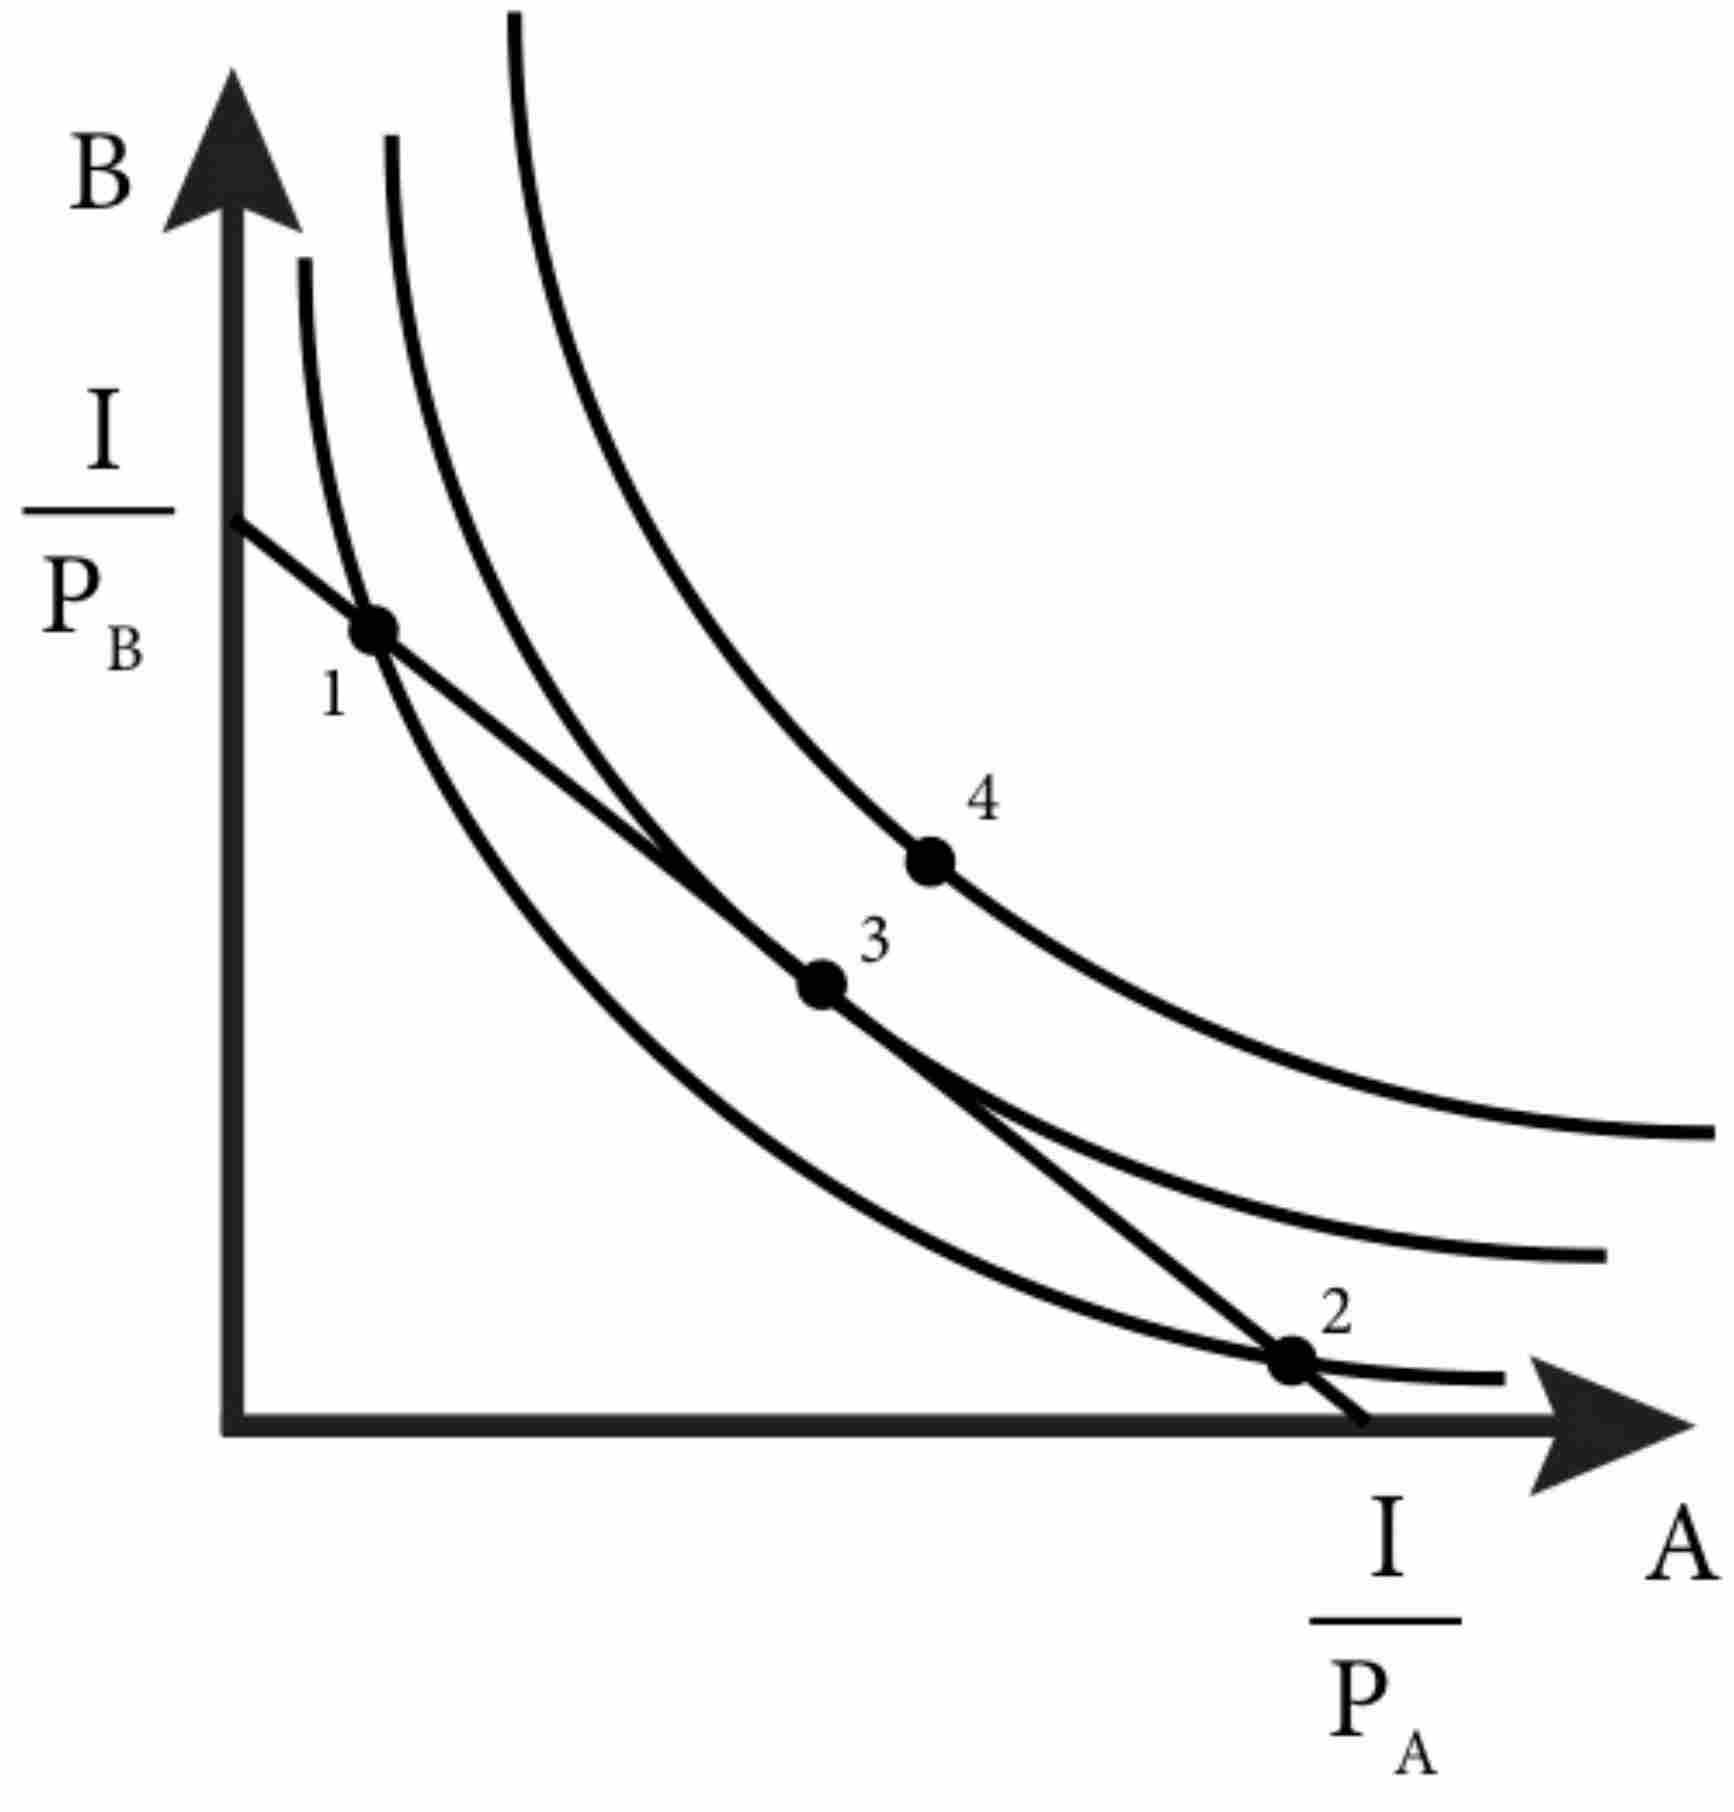
\includegraphics[width=0.5\textwidth,height=\textheight]{fig/utility-max.jpg}
\caption[\label{fig:utilmax} Utility maximization]{\label{fig:utilmax} Utility maximization\footnotemark{}}
\end{figure}
\footnotetext{This graph is taken from \citet[ch.~4]{Emerson2020Intermediate}}

Figure \ref{fig:utilmax} stems from \citet[ch.~4]{Emerson2020Intermediate}. Use the following sentences to describe the respective points in the figure.

\begin{itemize}
\tightlist
\item
  Optimal bundle.
\item
  Can do better by trading some B for some A.
\item
  Can do better by trading some B for some A.
\item
  Unaffordable.
\end{itemize}

Please find solutions to the exercise in \citet[ch.~4]{Emerson2020Intermediate}.
\end{exercise}

\hypertarget{markets-under-perfect-competition}{%
\section{Markets under perfect competition}\label{markets-under-perfect-competition}}

Perfect competition is never found in the real world. However, it is a useful theoretical model that serves as a reference point for analyzing real-world markets. It provides valuable insights into market functioning and informs policymakers on how to address instances of market failure, where at least one assumption of perfect markets is not met.

The assumptions of perfect markets and perfect competition, respectively, are:

\begin{enumerate}
\def\labelenumi{\arabic{enumi}.}
\item
  \textbf{Many buyers and sellers}: In a perfectly competitive market, there are numerous buyers and sellers, none of whom have a significant influence over market price. Each participant is a price taker, meaning they have no control over the price at which goods or services are exchanged.
\item
  \textbf{Homogeneous products}: The products offered by all firms in a perfectly competitive market are identical or homogeneous. Consumers perceive no differences between the goods or services provided by different sellers. As a result, buyers base their purchase decisions solely on price.
\item
  \textbf{Perfect information}: All buyers and sellers in a perfectly competitive market have complete and accurate information about prices, quality, availability, and other relevant factors. This assumption ensures that market participants can make rational decisions and respond efficiently to changes in market conditions.
\item
  \textbf{Free entry and exit}: Firms can freely enter or exit the market in response to profits or losses. There are no barriers to entry or exit, such as legal restrictions or substantial costs, that prevent new firms from entering the market or existing firms from leaving it.
\item
  \textbf{Perfect mobility of factors of production}: The resources used in production, such as labor and capital, can move freely between different firms and industries. There are no constraints on the mobility of factors of production, allowing firms to allocate resources efficiently.
\item
  \textbf{Profit maximization}: All firms in a perfectly competitive market are profit maximizers. They aim to maximize their profits by adjusting their output levels based on prevailing market conditions. If firms can increase their profits, they will expand production, and if they incur losses, they will reduce output or exit the market.
\item
  \textbf{No externatlities}: There are assumed to be no externalities, that is no external costs or benefits to third parties not involved in the transaction.
\end{enumerate}

These assumptions collectively define perfect competition and form the foundation of its analysis. If all conditions are fulfilled, there is no need for government regulation. Welfare is maximized and no pareto-improvement can be achieved.

Theory would predict that if firms in an industry would make some profits, new firms will enter the market or existing firms would produce more which both yields an increase in supply. That, in turn, will drive down market prices until all firms earn zero profits and no more firms would have an incentive to enter the market. In the equilibrium, total revenue equals total cost. Thus, firms do not make profits. Firms can only make profits if they have some sort of competitive advantage and hence are not price takers which would be against assumption 1. The most extreme form of competitive advantage is a monopoly. It describes that one firm is the only provider of a certain good or service. This firm can set prices and the supply of the good and service completely. We will discuss that extreme case in the next section.

\hypertarget{monopoly}{%
\section{Monopoly}\label{monopoly}}

A monopolist is a firm that is the only provider of a good or service. There is no close substitute to it.
The ability of a monopolist to raise its price above the competitive level by reducing output is known as \emph{market power}. This implies a loss of total welfare.
In contrast with a perfectly competitive firm which faces a perfectly elastic demand (taking
price as given), a monopolist faces the market demand. As a consequence, a monopolist has the power to set the market price. While we can consider a
competitive firm as a \emph{price taker}, a monopolist is price decision-maker or \emph{price setter}.
Firms that have to face fierce competition are more like price takers as they cannot set the price above the market price. If firms in perfect competition would set the price higher, all consumers would simply stop buying from that particular firm. That is not the case for a firm with market power, that is, a firm that has a product with unique features no other competitor has to offer.

\hypertarget{revenue-function}{%
\subsubsection*{Revenue function}\label{revenue-function}}
\addcontentsline{toc}{subsubsection}{Revenue function}

There are two types of constraints that restrict the behavior of a monopolist (and any other firm):

\begin{itemize}
\tightlist
\item
  Technological constraints summarized in the cost function \(C(x)\).
\item
  Demand constraints: \(x(p)\).
\end{itemize}

Thus, we can write the revenue (or profit) function of the monopolist in two alternative ways:

\begin{enumerate}
\def\labelenumi{\arabic{enumi}.}
\item
  Either by using the demand function:
  \[
  \pi(p) = px(p) - C(x(p))
  \]
\item
  Or by using the inverse demand function:
  \[
  \pi(x) = p(x)x - C(x)
  \]
\end{enumerate}

The demand, \(x(p)\), and the inverse demand, \(p(x)\), represent the same relationship between price and demanded quantity from different points of view. The demand function is a complete description of the demanded quantity at each price, whereas the inverse demand gives us the maximum price at which a given output \(x\) may be sold in the market.

\hypertarget{revenue-and-price-relationship}{%
\subsubsection*{Revenue and price relationship}\label{revenue-and-price-relationship}}
\addcontentsline{toc}{subsubsection}{Revenue and price relationship}

Thus, an increase in production by a monopolist has two opposing effects on revenue:

\begin{itemize}
\tightlist
\item
  A \textbf{quantity effect}: one more unit is sold, increasing total revenue by the price at which the unit is sold.
\item
  A \textbf{price effect}: in order to sell the last unit, the monopolist must cut the market price on all units sold. This decreases total revenue.
\end{itemize}

\begin{figure}
\centering
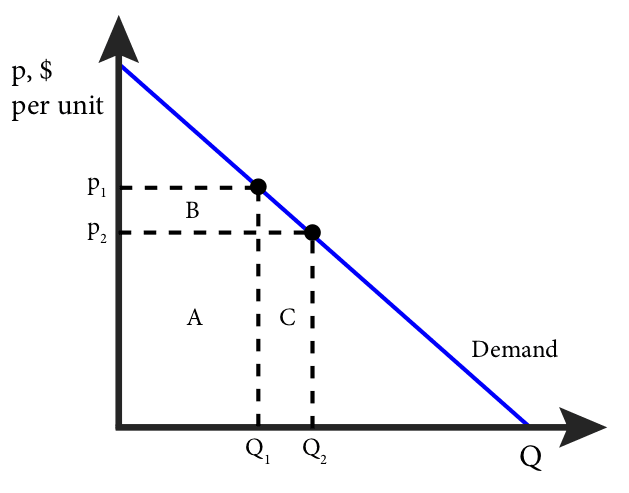
\includegraphics[width=0.4\textwidth,height=\textheight]{fig/revenue-mono.png}
\caption[\label{fig:revenue-mono} Price Effects and Revenue]{\label{fig:revenue-mono} Price Effects and Revenue\footnotemark{}}
\end{figure}
\footnotetext{Graph is taken from \citet{Emerson2020Intermediate}.}

The two effects are shown in figure \ref{fig:revenue-mono}: At price \(p_1\), the total revenue is \(p_1 \cdot Q_1\), which is represented by the areas A+B. At price \(p_2\), the total revenue is \(p_2 \cdot Q_2\), which is represented by the areas A+C. Area A is the same for both, so the marginal revenue is the difference between B and C or C-B. Note that area C is the price, \(p_2\), times the change in quantity, \(Q_2 - Q_1\), or \(p \Delta Q\); and area B is the quantity, \(Q_1\), times the change in price, \(p_2 - p_1\), or \(\Delta p \cdot Q\). Since \(p_2 - p_1\) is negative, the change in total revenue is C-B or: \(\Delta TR = p \Delta Q + \Delta p \cdot Q\). Dividing both sides by \(\Delta Q\) gives us an expression for marginal revenue:

\[
MR = \frac{\Delta TR}{\Delta Q} = \underbrace{p}_{\text{quantity effect}} + \underbrace{Q \frac{\Delta p}{\Delta Q}}_{\text{price effect}}
\]

\hypertarget{profit-maximizing-level-of-output}{%
\subsubsection*{Profit-maximizing level of output}\label{profit-maximizing-level-of-output}}
\addcontentsline{toc}{subsubsection}{Profit-maximizing level of output}

To find the profit-maximizing price and quantity, respectively, we should look at the first-order conditions:

\begin{align*}
\max_{p} \pi (p) \equiv& \max_{p} \quad px(p) - C(x(p))\\
\frac{\partial \pi (p)}{\partial p} =& \pi ' (p) = x(p) + px'(p) - C'(x(p))x'(p) \overset{!}{=} 0
\end{align*}

or

\begin{align*}
\max_{p} \pi (x) \equiv& \max_{x} \quad p(x)x - C(x)\\
\frac{\partial \pi (x)}{\partial x} =& \pi ' (p) = \underbrace{p(x)}_{\text{quantity effect}} + \underbrace{xp'(x)}_{\text{price effect}} - C'(x) \overset{!}{=}& 0\\
\Rightarrow \underbrace{p(x) + xp'(x)}_{\text{marginal revenue}} =& \underbrace{C'(x)}_{\text{marginal costs}}\\
\Rightarrow MR =& MC
\end{align*}

At the profit-maximizing level of output, \textbf{marginal revenue equals marginal cost}, that is, an infinitesimal change in the level of output changes revenue and cost equally. In other words, an infinitesimal increase in the level of output increases revenue and cost by the same amount, and an infinitesimal decrease in the level of output reduces revenue and cost by the same amount.

Thus, we can determine a monopoly firm's profit-maximizing price and output by following three steps:

\begin{enumerate}
\def\labelenumi{\arabic{enumi}.}
\tightlist
\item
  Determine the demand, marginal revenue, and marginal cost curves.
\item
  Select the output level at which the marginal revenue and marginal cost curves intersect.
\item
  Determine from the demand curve the price at which that output can be sold.
\end{enumerate}

\hypertarget{price-effect-of-a-monopoly}{%
\subsubsection*{Price effect of a monopoly}\label{price-effect-of-a-monopoly}}
\addcontentsline{toc}{subsubsection}{Price effect of a monopoly}

Due to the price effect of an increase in output, the marginal revenue curve of a firm with market power always lies below its demand curve. So, a profit-maximizing monopolist chooses the output level at which marginal cost is equal to marginal revenue---not equal to price. As a result, the monopolist \textbf{produces less and sells its output at a higher price than a perfectly competitive industry would}. It earns a profit in the short run and the long run.

\hypertarget{welfare}{%
\subsubsection*{Welfare}\label{welfare}}
\addcontentsline{toc}{subsubsection}{Welfare}

As illustrated in Figure \ref{fig:mono2}, the price-setting behavior of a monopolist typically leads to a reduction in overall welfare: The shaded green area represents the \emph{monopoly profit}, and the blue area denotes the \emph{consumer surplus}, the sum of both constitute the total welfare. The yellow triangle represents the deadweight loss, indicating the welfare that is lost due to the monopolist producing fewer goods at a higher price than in a competitive market. The horizontal line at \(p=100\) represents the marginal costs (MC).

\begin{figure}
\centering
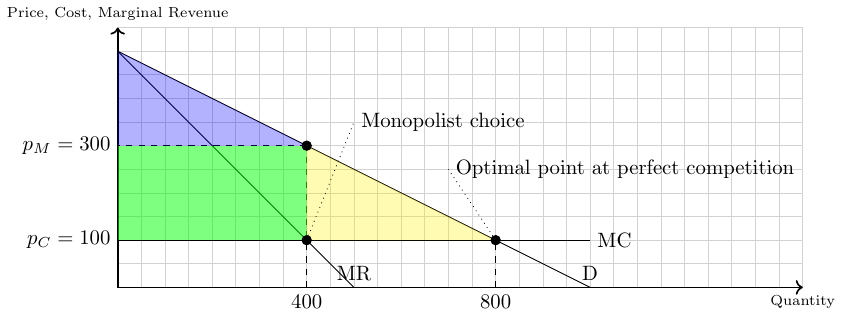
\includegraphics[width=1\textwidth,height=\textheight]{fig/monopoly.png}
\caption{\label{fig:mono2} Price setting of a monopolist}
\end{figure}

\hypertarget{price-elasticity-and-market-power}{%
\subsubsection*{Price elasticity and market power}\label{price-elasticity-and-market-power}}
\addcontentsline{toc}{subsubsection}{Price elasticity and market power}

We know that the demand elasticity of price can be measured with:

\[ \frac{\triangle p/\bar{p}}{\triangle x / \bar{x}}. \]

Using differential calculus, the point-price elasticity of demand (PPD) can be written as:

\[ PPD = \frac{\partial p(x)}{\partial x} \cdot \frac{x}{p(x)} \]

This can also be expressed as:

\[ PPD = p'(x) \frac{x}{p(x)} = x \frac{p'(x)}{p(x)} \]

Thus, if \(PPD = 0\), the price does not change if a single firm increases its quantity sold on the market. That means the firms are price takers, and their quantity sold has no impact on the price. If firms, however, have market power, \(PPD < 0\), which means that if a firm increases the quantity on the market, the price must fall. \textbf{The PPD can hence be interpreted as an indicator of the market power of firms.}

\hypertarget{marginal-revenue-and-price-elasticity}{%
\subsubsection*{Marginal revenue and price elasticity}\label{marginal-revenue-and-price-elasticity}}
\addcontentsline{toc}{subsubsection}{Marginal revenue and price elasticity}

Now, plugging the PPD into the MR function, we can show that MR is equal to zero when we have a unit demand elasticity, PPD, of \(-1\):

\[ MR = p(x) + xp'(x) = p(x)\left(1 + x\frac{p'(x)}{p(x)}\right) = p(x)\left(1 + PPD\right) \]

Also see figure \ref{fig:ppd}. In the monopoly output, marginal revenue and marginal cost are equal:

\[ MC = p(x) \cdot \left(1 + PPD\right) \]

\begin{figure}
\centering
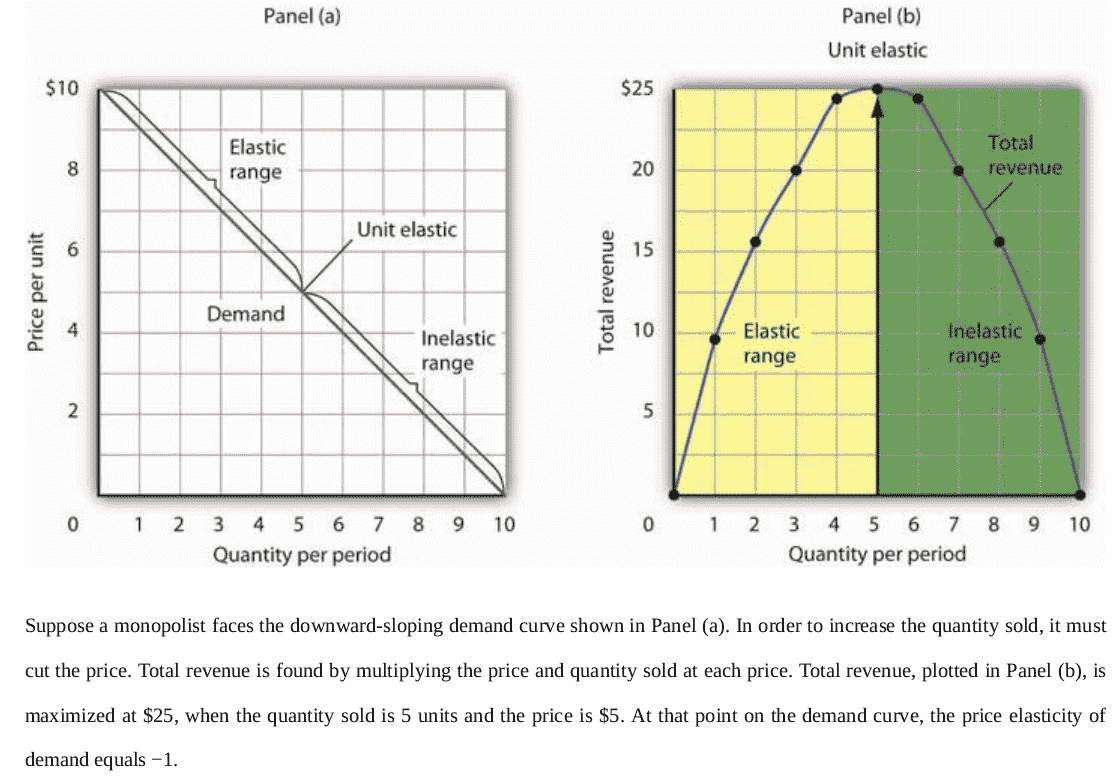
\includegraphics[width=0.75\textwidth,height=\textheight]{fig/ppd.png}
\caption[\label{fig:ppd} Price setting of a monopolist]{\label{fig:ppd} Price setting of a monopolist\footnotemark{}}
\end{figure}
\footnotetext{Graph stems from \citet[p.~344]{Anonymous2020Principles}}

\hypertarget{lerner-index}{%
\subsubsection*{Lerner index}\label{lerner-index}}
\addcontentsline{toc}{subsubsection}{Lerner index}

The Lerner index is a measure of monopoly power, which equals the markup over marginal cost as a percentage of price. To obtain the Lerner index of monopoly power (or market power), let us rearrange \(MC = p(x) \cdot \left(1 + PPD\right)\) as follows:

\[ \frac{MC - p(x)}{p(x)} = PPD = \text{Lerner Index} \]

If a firm does not have market power (\(PPD = 0\)), its price equals the marginal cost. When a firm's market power is high (up to \(|PPD| = \infty\)), the higher the markup that a firm sets. In perfect competition, since \(p\) and MC are equal, the Lerner Index is 0. A pure monopolist, on the other hand, can theoretically charge an infinite markup, which leads us to a Lerner index of 1.

\begin{center}\rule{0.5\linewidth}{0.5pt}\end{center}

\begin{exercise}
\protect\hypertarget{exr:marrevtotrev}{}\label{exr:marrevtotrev}Marginal revenue and total revenue

Show the relationship between a linear demand curve and the marginal revenue curve in one panel and the relationship of the quantity sold and the total revenue in another panel. What characterizes the price of a profit maximizing monopolist?

Please find solution to the exercise \protect\hyperlink{sol:marrevtotrev}{in the appendix.}
\end{exercise}

\begin{exercise}
\protect\hypertarget{exr:howtomaxprofit}{}\label{exr:howtomaxprofit}How to maximize profits

A company sold a quantity of 750 goods (\(Q_{t=1}=750\)) in January (\(t=1\)), at a price of 45 € (\(P_{t=1}=45\)). In February (\(t=2\)), they reduced the price to 40 Euro (\(P_{t=2}=40\)) and sold 800 goods (\(Q_{t=2}=800\)). Now answer the following questions knowing that the total costs had been 26,500 € in January and 28,000 € in February.

\begin{enumerate}
\def\labelenumi{\arabic{enumi}.}
\tightlist
\item
  Calculate the price elasticity of demand at the current prices.
\item
  Derive the demand function.
\item
  Derive the cost function.
\item
  Derive the revenue function.
\item
  Derive the marginal revenue function.
\item
  Derive the marginal cost function.
\item
  Calculate the profit-maximizing price and output.
\item
  Calculate the amount of profit in January, February, and what the company can expect by setting the prices profit-maximizing.
\end{enumerate}

Please find solution to the exercise \protect\hyperlink{sol:howtomaxprofit}{in the appendix.}
\end{exercise}

\hypertarget{monopoly-and-price-discrimination}{%
\subsection{Monopoly and price discrimination}\label{monopoly-and-price-discrimination}}

Discrimination is the practice of treating people differently based on some (irrelevant) characteristic, such as race or gender. It is important to actively fight discrimination whenever it is observed. However, the concept of discrimination takes a different form when it comes to \emph{price discrimination}, which is a business practice involving the sale of the same goods at different prices to different buyers. This practice can be commonly seen in special offers tailored for students or retired individuals.

One of the key factors utilized in price discrimination is the willingness to pay (WTP) of individuals. By charging a higher price to buyers with a higher WTP, a firm can maximize its profit. Moreover, and that is kind of surprising, it also comes with a increase in social welfare as is shown in figure \ref{fig:monowpd} and figure \ref{fig:monowpd}. In \ref{fig:monowpd}, the monopolist charges the same price (PM) to all buyers. A deadweight loss results. In \ref{fig:monowpd}, however, the monopolist produces the competitive quantity but charges each buyer his or her WTP. This is called perfect price discrimination. The monopolist captures all consumer surplus as profit. But there is no deadweight loss.

\begin{figure}
\centering
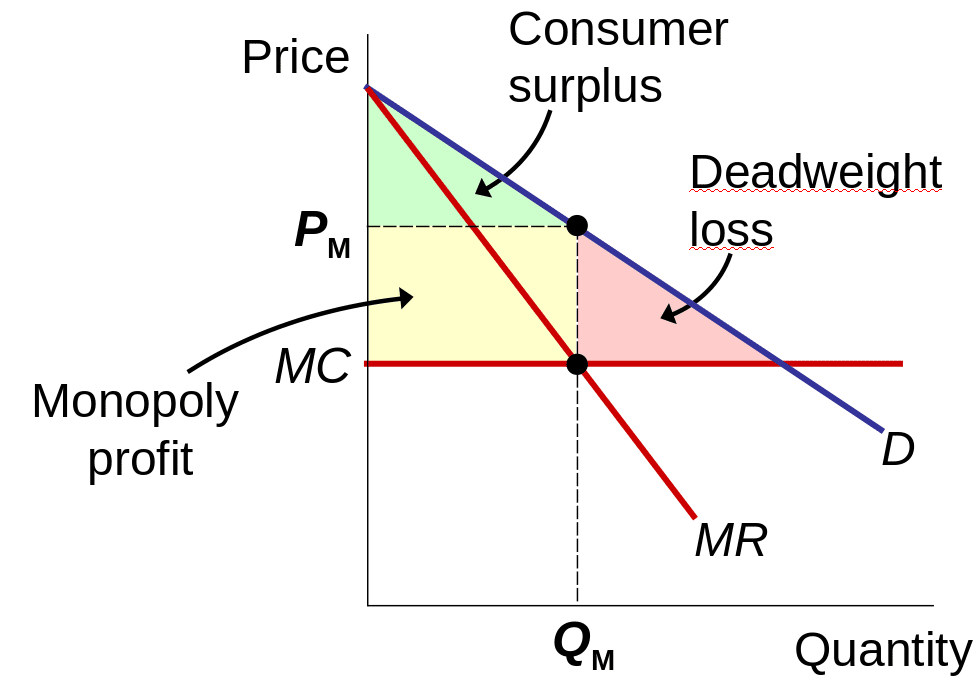
\includegraphics[width=0.35\textwidth,height=\textheight]{fig/discrimination.png}
\caption{\label{fig:monowoutpd} Monopoly without price discrimination and welfare}
\end{figure}

\begin{figure}
\centering
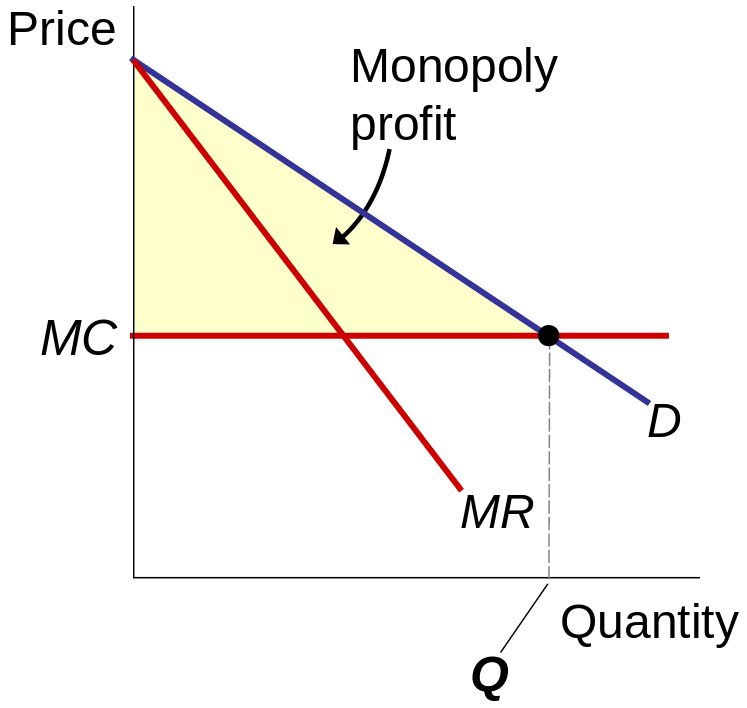
\includegraphics[width=0.25\textwidth,height=\textheight]{fig/discrimination2.png}
\caption{\label{fig:monowpd} Monopoly with price discrimination and welfare}
\end{figure}

In the real world, price discrimination is a common phenomenon, but achieving perfect price discrimination is highly challenging. This is primarily because no firm possesses complete knowledge of every buyer's willingness to pay (WTP), and buyers typically do not disclose this information to sellers. Consequently, firms often divide customers into groups based on observables that are likely correlated with their WTP.

\hypertarget{regional-economics}{%
\section{Regional Economics}\label{regional-economics}}

\hypertarget{von-thuxfcnen-model-of-land-use}{%
\subsection{Von Thünen model of land use}\label{von-thuxfcnen-model-of-land-use}}

The classical model of spatial organization of the economy stems Heinrich von Thünen (1783-1850). The model focuses on agriculture as this was the dominant use of land at the time. However, the fundamental ideas of the model can be applied to various industries.
The model can be described as follows: Assume a focal point of demand for agricultural goods (e.g., the marketplace of a large city). Differences in soil quality in the agricultural periphery of the considered city are neglected. The demand is differentiated. That means, various goods such as grains, dairy products, meat, timber, vegetables are required to satisfy the needs of the people. The goods differ in terms of

\begin{itemize}
\tightlist
\item
  the market price they can achieve,
\item
  the assumed constant marginal production costs \((c_i)\),
\item
  the revenue per unit of land, and
\item
  in terms of their transportability, that is, each good has different specific transport costs \((\theta_i)\).
\end{itemize}

All mentioned variables are exogenously given. In particular, the model is based on the following assumptions:

\begin{enumerate}
\def\labelenumi{\arabic{enumi}.}
\tightlist
\item
  Point-centered demand for all goods \(i\).
\item
  Different production methods possible, each with constant (marginal) production costs \(c_i\).
\item
  Homogeneous Space: The agricultural land surrounding the central marketplace is assumed to be uniform and homogeneous in terms of soil fertility, climate, and other relevant factors.
\item
  Given market prices for the individual products \(p_i\)
\item
  Producers supply the market and have linear product-specific transportation costs \((\theta_i)\).
\item
  Perfect competition: The model assumes perfect competition among farmers for the available land (free market access). That implies that they have full knowledge of market conditions and make rational decisions.
\end{enumerate}

To analyze the model, let us start by considering the restriction to a single land use. The key idea is that the rent price for a unit of land arises from the net yield that this unit of land enables under that particular land use. However, since both production costs and distance-dependent transport costs need to be subtracted from the gross yield to determine the net yield, it follows that land rent is determined by the distance from the center. Under a given land use, the value of an agricultural area is significantly influenced by its distance from the marketplace.

Formally, the land rent for land use for production of good \(i\), depending on the distance \(x\) from the marketplace, is given by:

\[
r_i(x) = q_i(p_i - c_i - \theta_i \cdot x)
\]

The land rent increases with the quantity demanded \((q)\) and the price of the good, and it decreases with the marginal production costs \((c)\), the specific transportation costs \((\theta)\), and the distance \((x)\) from the marketplace. The typical shape of a rent curve, with \(r\) on the y-axis and \(x\) on the x-axis, is a linearly decreasing curve. Its slope is determined by the expression \(-q_i \theta_i\). Therefore, the steeper the specific transportation costs, the steeper the curve.

Suppose, different land uses are allowed. By varying the price, revenue, and cost parameters in the equation above, different rent curves with varying locations and slopes emerge for different land uses. The interesting question now is: \emph{How high will the market rent be?}

Thünen provides a clear answer to this question: Competition among land tenants will ensure that in a specific distance zone around the center, the production method with the highest net yield in that zone will prevail. In other words, the market rent curve (or bid rent curve) is the upper envelope of all rent curves for specific production methods. The situation is illustrated in figure \ref{fig:thuenen} and \ref{fig:thuenen2} for three different production methods. The intersections of the market rent curves determine the shifts in production zones.

\begin{figure}
\centering
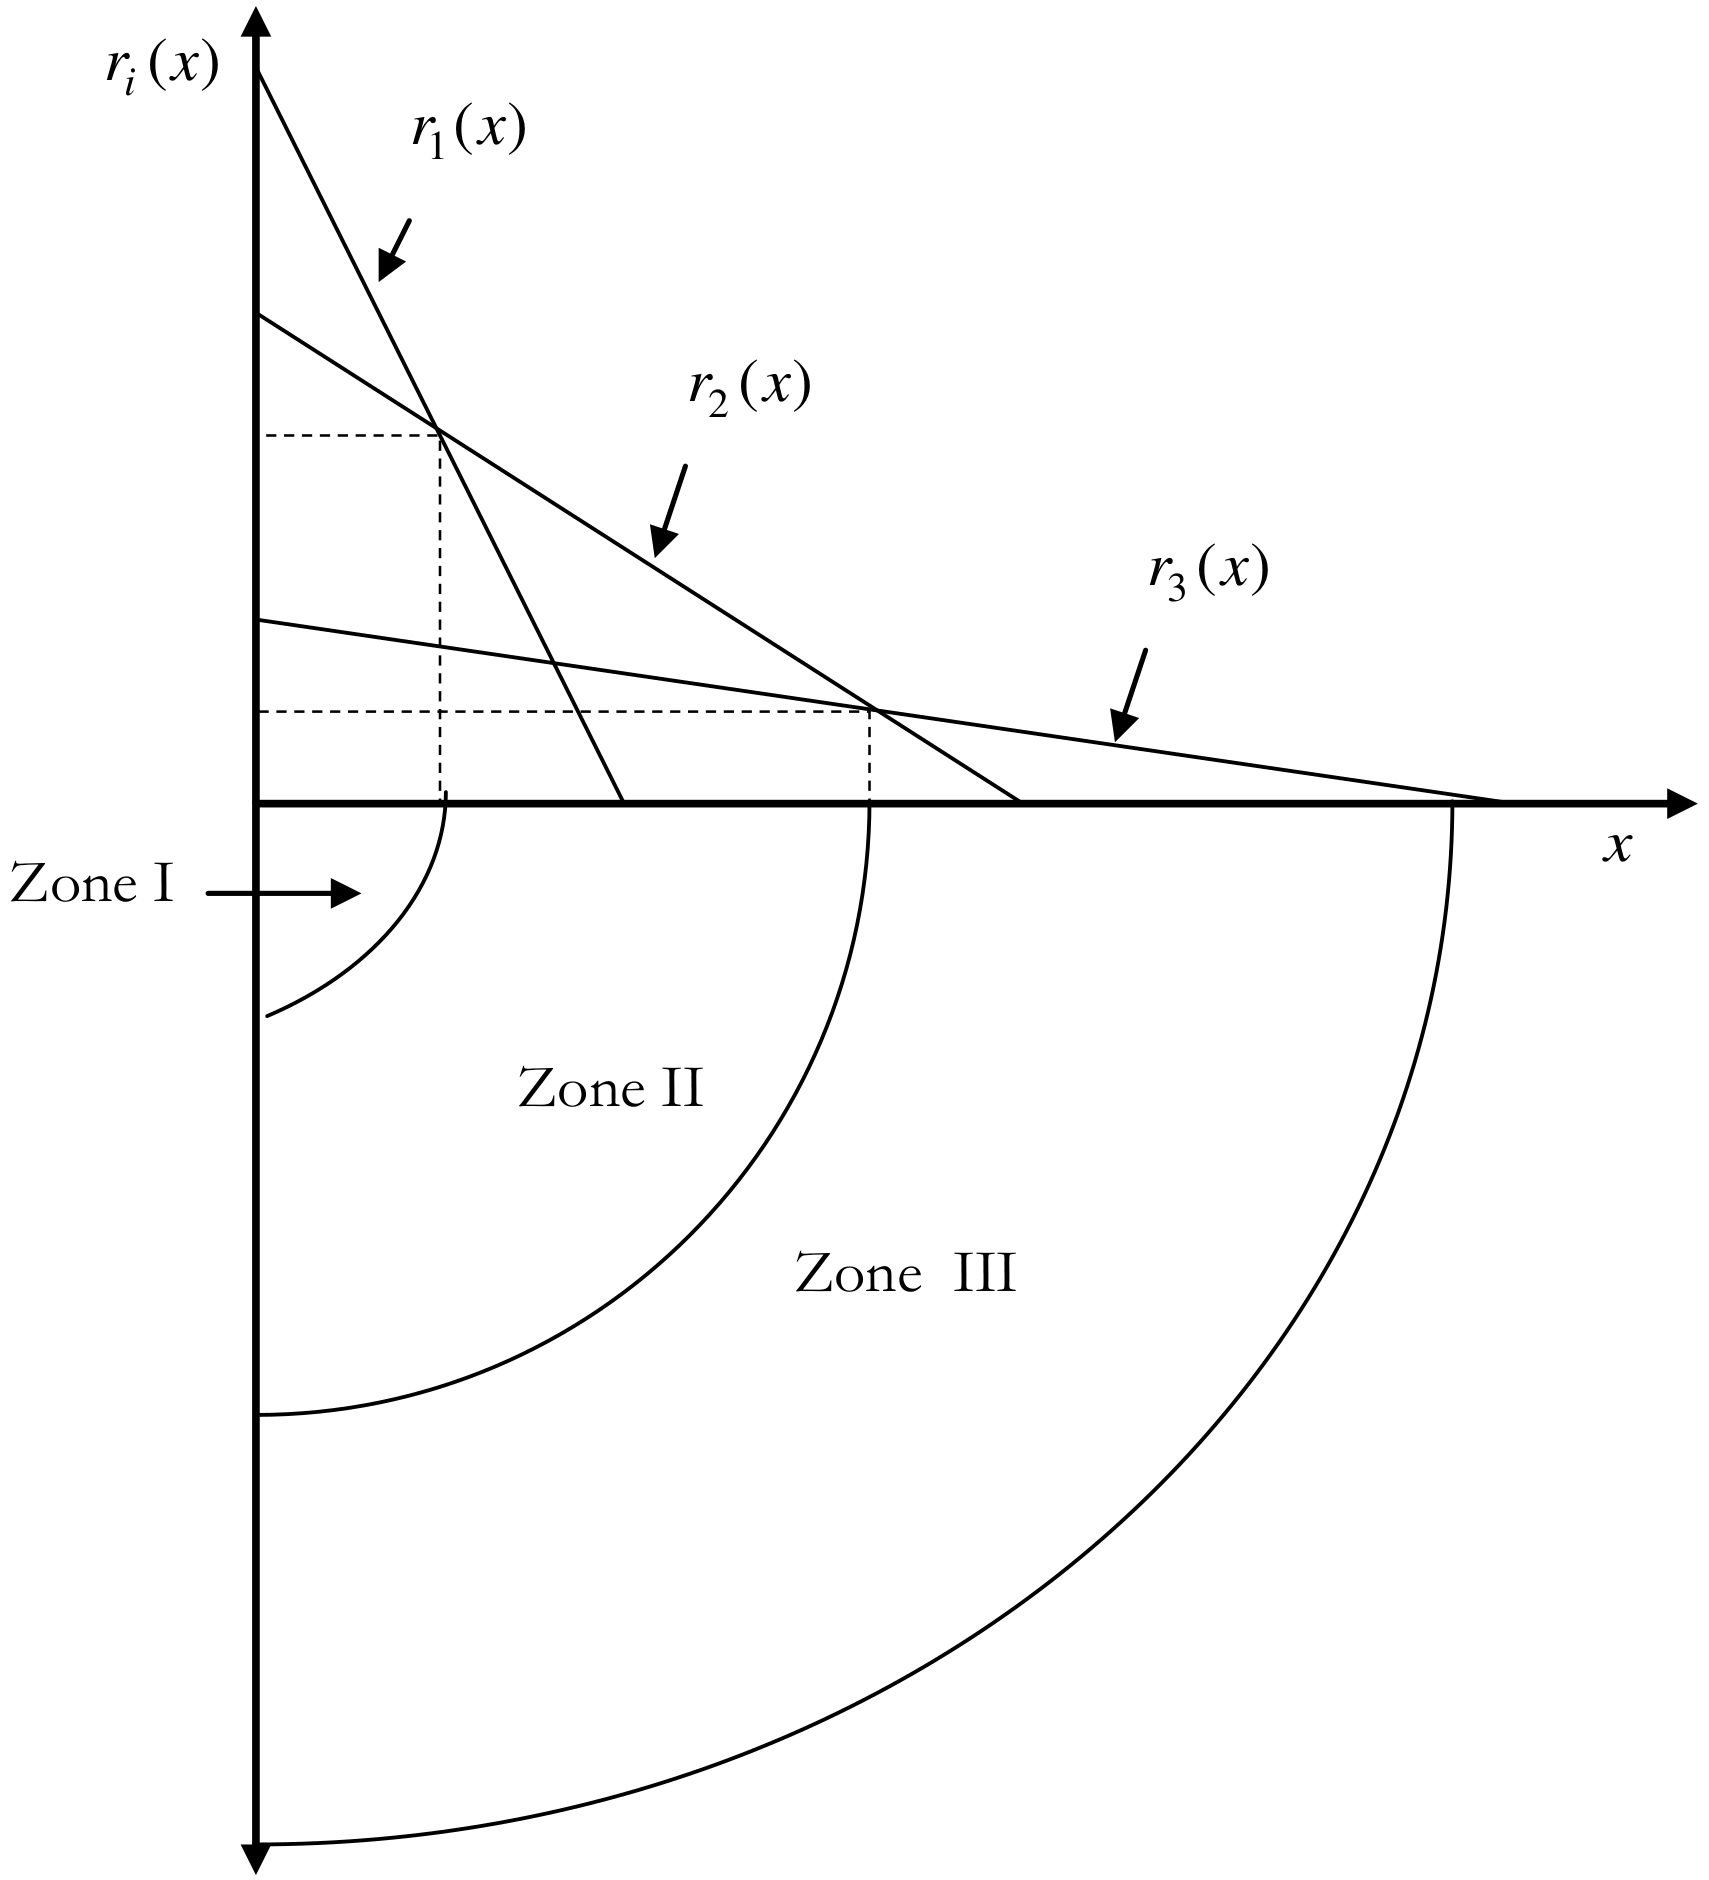
\includegraphics[width=0.6\textwidth,height=\textheight]{fig/thuenen.png}
\caption{\label{fig:thuenen} Thünen's rings of land use}
\end{figure}

\begin{figure}
\centering
\includegraphics[width=0.6\textwidth,height=\textheight]{fig/Bid_rent1.png}
\caption[\label{fig:thuenen2} Bid rent curve]{\label{fig:thuenen2} Bid rent curve\footnotemark{}}
\end{figure}
\footnotetext{The graph stems from \url{https://en.wikipedia.org/wiki/File:Bid_rent1.png}}

This model is also known as the \emph{Bid rent theory}. A short but nice explanation of the model can be found on Wikipedia, see \href{https://en.wikipedia.org/wiki/Bid_rent_theory}{here}.

\begin{center}\rule{0.5\linewidth}{0.5pt}\end{center}

\begin{exercise}
\protect\hypertarget{exr:thuenen1}{}\label{exr:thuenen1}

Agricultural land use

In the vicinity of an agglomeration center, four different agricultural land use forms are possible. We have information about the specific yield per unit of land \(q_i\), the (constant) marginal costs \(c_i\), the specific transportation costs \(\theta_i\), and the price \(p_i\) that can be achieved for a unit of the respective product in the center.

Where do we see which land use form?

\begin{longtable}[]{@{}
  >{\raggedright\arraybackslash}p{(\columnwidth - 8\tabcolsep) * \real{0.0588}}
  >{\raggedright\arraybackslash}p{(\columnwidth - 8\tabcolsep) * \real{0.2353}}
  >{\raggedright\arraybackslash}p{(\columnwidth - 8\tabcolsep) * \real{0.2353}}
  >{\raggedright\arraybackslash}p{(\columnwidth - 8\tabcolsep) * \real{0.2353}}
  >{\raggedright\arraybackslash}p{(\columnwidth - 8\tabcolsep) * \real{0.2353}}@{}}
\toprule\noalign{}
\begin{minipage}[b]{\linewidth}\raggedright
\end{minipage} & \begin{minipage}[b]{\linewidth}\raggedright
Production Form
\end{minipage} & \begin{minipage}[b]{\linewidth}\raggedright
Production Form
\end{minipage} & \begin{minipage}[b]{\linewidth}\raggedright
Production Form
\end{minipage} & \begin{minipage}[b]{\linewidth}\raggedright
Production Form
\end{minipage} \\
\midrule\noalign{}
\endhead
\bottomrule\noalign{}
\endlastfoot
\(i\) & 1 & 2 & 3 & 4 \\
\(q_i\) & 10 & 5 & 30 & 20 \\
\(p_i\) & 5 & 5 & 2 & 6 \\
\(c_i\) & 1 & 2 & 1 & 5 \\
\(\theta_i\) & 0.4 & 0.1 & 0.15 & 0.05 \\
\end{longtable}

\end{exercise}

\begin{exercise}
\protect\hypertarget{exr:thuenen2}{}\label{exr:thuenen2}Business location model

The Thünenian approach is intended to be applied to a business location model. The customer frequency, depending on the distance \(x\) from the center, can be approximated by the following function:

\[ f(x)_i = A_{0} e^{-a x} \]

The probability of sale per square meter for business type \(i\) is denoted by \(\lambda_i\). The business types also differ in terms of profit margin and fixed costs. Describe the market rent curve and show which business type will dominate in each location. What effects does an increase in the parameter \(a\) have? What about an increase in \(A_0\)? Interpret the changes in parameters and the results from an economic perspective.
\end{exercise}

\hypertarget{launhardthotelling-location-model}{%
\subsection{Launhardt/Hotelling location model}\label{launhardthotelling-location-model}}

Consider a scenario where two firms, i.e., \(i={F1;F2}\), have the option to establish their locations along a linear market, such as a street or a beach. These firms can relocate without incurring any costs and sell an identical product at the same price. Consequently, the only means of competition available to them is by strategically selecting their respective locations.
Moreover, assume that customers are uniformly distributed throughout the market, and each customer is willing to purchase one unit of the product up to a certain price, denoted as \(\bar{p}\). The cost of transportation is the same for both firms and is proportional to the distance between the firm and the customer.

If we assume that the transportation costs are equal for both firms and that the market has a finite size, the firms will eventually position themselves at the center of the market with no empty space between them. The rationale and dynamics behind this behavior are clearly explained in the YouTube clip of TED-Ed \href{https://youtu.be/jILgxeNBK_8}{\emph{Why do competitors open their stores next to one another? - Jac de Haan}}, see figure \ref{fig:hotelling}. I highly recommend watching the clip.

\begin{figure}
\centering
\includegraphics[width=0.25\textwidth,height=\textheight]{fig/hotelling.png}
\caption[\label{fig:hotelling} YouTube clip of TED-Ed and Jac de Haan]{\label{fig:hotelling} YouTube clip of TED-Ed and Jac de Haan\footnotemark{}}
\end{figure}
\footnotetext{Taken from \url{https://youtu.be/jILgxeNBK_8}}

If we assume that the transportation costs can vary between the two firms, things became a bit more complicated. Let us define transportation costs for a firm as \(\theta_i=a_i d(x)\), where \(d(x)\) represents the distance between the company and the respective costumer and \(a_i\) is firm-specific costs of transportation. Let us further assume competition and loosen the assumption of fixed prices: Firms can set prices but they need to charge the price of the good, \(p\), plus their costs of transporting the good to the costumer. Thus, the price of a good a firm needs to charge in order not to make deficits is
\[
p^{min}(x)=c+\theta_i=c+a_i d(x)
\]

If we assume that the transport costs are the same for both firms and that the market is limited in size, the firms will end up at the center of the market with no space inbetween them. However, there is always an incentive to deviate from that minimum of spatial differentiation. However, the dynamic is kind of strange as we can show in the following four figures.

\begin{figure}
\centering
\includegraphics[width=0.75\textwidth,height=\textheight]{fig/lau1.png}
\caption{\label{fig:lau1} Scenario 1}
\end{figure}

\begin{figure}
\centering
\includegraphics[width=0.75\textwidth,height=\textheight]{fig/lau2.png}
\caption{\label{fig:lau2} Scenario 2}
\end{figure}

\begin{figure}
\centering
\includegraphics[width=0.75\textwidth,height=\textheight]{fig/lau3.png}
\caption{\label{fig:lau3} Scenario 3}
\end{figure}

\begin{figure}
\centering
\includegraphics[width=0.75\textwidth,height=\textheight]{fig/lau4.png}
\caption{\label{fig:lau4} Scenario 4}
\end{figure}

\hypertarget{appendix}{%
\chapter{Appendix}\label{appendix}}

\hypertarget{micro-pre}{%
\section{Microeconomic preliminaries}\label{micro-pre}}

In this appendix, I will cover several microeconomic preliminaries that are crucial for your understanding. These include:

\begin{enumerate}
\def\labelenumi{\arabic{enumi}.}
\tightlist
\item
  Production Possibility Frontier (PPF): I will explain how the PPF curve graphically visualizes the production and growth of firms and countries.
\item
  Indifference curves: I will discuss how indifference curves represent different bundles of goods at which consumers are indifferent.
\item
  Budget constraints: I will show you how to graphically sketch budget constraints, which play a significant role in consumer decision-making.
\item
  Consumption choices: I will explore how the concepts of PPF, indifference curves, and budget constraints come together to explain consumer consumption choices.
\item
  Competitive market prices: I will explain how prices on competitive markets are determined through the interaction of producers and consumers.
\end{enumerate}

\hypertarget{production-possibility-frontier-curve}{%
\subsection{Production possibility frontier curve}\label{production-possibility-frontier-curve}}

\begin{figure}
\centering
\includegraphics[width=0.3\textwidth,height=\textheight]{fig/ppf1.png}
\caption{\label{fig:ppf} The production possibility frontier curve}
\end{figure}

The production possibility frontier curve (PPF) as shown in figure \ref{fig:ppf} provides a graphical representation of all possible output options for two products when all available resources and factors of production are fully and efficiently utilized within a given time frame. The PPF serves as the boundary between combinations of goods and services that can be produced and those that cannot.

The PPF is an invaluable tool for illustrating the implications of scarcity, as it offers insights into production efficiency, opportunity costs, and tradeoffs between different choices. Typically, the PPF exhibits concavity since not all factors of production can be used equally productive in all activities.

\emph{Economic growth} refers to the sustained expansion of production possibilities. An economy experiences growth through advancements in technology, enhancements in labor quality, or increases in capital quantity. As an economy`s resources increase, its production possibilities expand, causing the PPF to shift outward. It is worth noting that you can use the PPF to explain production in an ``economy'' or in a ``firm'', respectively.

\emph{Production efficiency} arises when it is impossible to produce more of one good or service without producing less of another. When production occurs directly on the PPF, it signifies efficiency. On the other hand, if production takes place inside the PPF, there is potential to produce more goods without sacrificing any existing ones, indicating inefficiency. When production lies on the PPF, a tradeoff emerges because obtaining more of one good necessitates giving up some quantity of another. This tradeoff incurs a cost, known as an \emph{opportunity cost}.

\begin{exercise}
\protect\hypertarget{exr:Uproduction}{}\label{exr:Uproduction}Understanding production

\begin{enumerate}
\def\labelenumi{\alph{enumi})}
\tightlist
\item
  Figure \ref{fig:ppf2} shows a PPF and five conceivable production points, \(C_i\), where \(i\in \{1,\dots,5\}\).
  Explain the figure using the following terms: \emph{attainable point; available resources, unattainable, inefficient, efficient point}.
\end{enumerate}

\begin{figure}
\centering
\includegraphics[width=0.3\textwidth,height=\textheight]{fig/ppf2.png}
\caption{\label{fig:ppf2} Production and different consumptions points}
\end{figure}

\begin{enumerate}
\def\labelenumi{\alph{enumi})}
\setcounter{enumi}{1}
\item
  What would happen to the PPF if the technology available in a country and needed for the production process became better?
\item
  What would happen to the PPF if the resources available in a country and needed in the production process of both goods shrank?
\item
  What would happen to the PPF if the resources (technology) available in a country that are needed in the production process\(\dots\)

  \begin{enumerate}
  \def\labelenumii{\roman{enumii})}
  \tightlist
  \item
    \(\dots\) for both goods increased (improved)?
  \item
    \(\dots\) for good A shrank (got worse)?
  \item
    \(\dots\) for good B increased (improved)?
  \end{enumerate}
\item
  Does the shape of the PPF tell us anything about economies of scale in the production process?
\item
  Figure \ref{fig:ppf3} shows an extreme PPF. How can such a PPF be explained?
\end{enumerate}

\begin{figure}
\centering
\includegraphics[width=0.2\textwidth,height=\textheight]{fig/ppf3.png}
\caption{\label{fig:ppf3} Extreme production possibility frontier curve}
\end{figure}

Please find solution to the exercise \protect\hyperlink{sol:Uproduction}{in the appendix.}

\hypertarget{indifference-curves-and-isoquants}{%
\subsection{Indifference curves and Isoquants}\label{indifference-curves-and-isoquants}}

\begin{figure}
\centering
\includegraphics[width=0.25\textwidth,height=\textheight]{fig/ic1.png}
\caption{\label{fig:ic1} Indifference curve}
\end{figure}

Combinations of two goods that yield the same level of utility for consumers are represented by indifference curves, see figure \ref{fig:ic1}. These curves illustrate the various bundles of goods where consumers are equally satisfied. That means all points on an indifference curve represent the same level of utility. The shape of the indifference curve is determined by the underlying utility function, which captures the preferences of consumers for consuming different combinations of the two goods.

The slope of an indifference curve indicates the rate at which the two goods can be substituted while maintaining the same level of utility for the consumer. Technically, the slope represents the marginal rate of substitution, which is equal to the absolute value of the slope. It measures the maximum quantity of one good that a consumer is willing to give up in order to obtain an additional unit of the other good.

It is assumed that consumers aim to attain the highest possible indifference curve because a higher curve, located further to the right on a coordinate system, represents a higher level of utility. In figure \ref{fig:ic2} for example, \(IC_1\) represents a lower level of utility than \(IC_2\).

\begin{figure}
\centering
\includegraphics[width=0.3\textwidth,height=\textheight]{fig/ic2.png}
\caption{\label{fig:ic2} Indifference curve}
\end{figure}

Similar to the concept of indifference curves, an \textbf{isoquant} shows the combinations of factors of production that result in the same quantity of output.
\end{exercise}

\begin{figure}

{\centering \includegraphics[width=0.6\linewidth]{_main_files/figure-latex/isocom-1} 

}

\caption{Perfect complements or substitutes}\label{fig:isocom}
\end{figure}

\begin{exercise}
\protect\hypertarget{exr:isoquants}{}\label{exr:isoquants}Isoquants

\begin{enumerate}
\def\labelenumi{\alph{enumi})}
\item
  Which of the two plots of figure \ref{fig:isocom} show isoquants when factors of production are \textbf{perfect complements} and \textbf{perfect substitutes}, respectively?
\item
  Discuss the features of a Cobb-Douglas PF with respect to returns to scale and marginal product of production for both inputs. Sketch the total output curve in an output-\(K\) and an output-\(L\) quadrant. Sketch the isoquants for different levels of production.
\end{enumerate}

Please find solution to the exercise \protect\hyperlink{sol:isoquants}{in the appendix.}
\end{exercise}

\hypertarget{budget-constraint}{%
\subsection{Budget constraint}\label{budget-constraint}}

In microeconomics, the concept of a budget constraint plays a vital role in understanding consumer decision-making and helps to analyze consumer choices and trade-offs. The budget constraint represents the limitations faced by consumers in allocating their limited income across different goods and services. The budget constraint indicates that the total expenditure on goods and services, calculated by multiplying the prices of each item by its corresponding quantity, must be less than or equal to the consumer's income.
Mathematically, the budget constraint can be expressed as:
\[
P_1 \cdot Q_1 + P_2 \cdot Q_2 + \ldots + P_n \cdot Q_n \leq I
\]
where \(P_n\) represent the prices of goods, \(Q_n\) denote the quantities of goods \(n\) consumed. \(I\) denotes the consumer's income or their \emph{budget}.

Consumers strive to maximize their utility by selecting the optimal combination of goods and services within the constraints imposed by their limited income. This involves making decisions about how much of each good to consume while staying within the budgetary limits. The graphical representation of the ideal consumption point is depicted in Figure \ref{fig:pointofconsumption}.

By studying the budget constraint, economists can gain insights into consumer behavior, price changes, and the impact of income fluctuations on consumption patterns.

\begin{figure}
\centering
\includegraphics[width=0.4\textwidth,height=\textheight]{fig/pointofconsumption.png}
\caption{\label{fig:pointofconsumption} Indifference curve}
\end{figure}

\hypertarget{logarithmic-and-exponential-function}{%
\section{Logarithmic and exponential function}\label{logarithmic-and-exponential-function}}

\begin{figure}
\centering
\includegraphics[width=0.3\textwidth,height=\textheight]{fig/logexp1.png}
\caption{\label{fig:logexp1} Logarithmic and exponential function}
\end{figure}

\begin{figure}
\centering
\includegraphics[width=0.3\textwidth,height=\textheight]{fig/logexp2.png}
\caption{\label{fig:logexp2} Logarithmic and exponential function zoomed in}
\end{figure}

\hypertarget{logarithmic-function}{%
\subsection{Logarithmic function}\label{logarithmic-function}}

Maybe you have heard about the logarithm, and I'm quite sure you know the `log' button on your calculator. If you wonder what it actually is and why it is so important for calculating with growth rates, this section is for you.

Consider the following equations and then explain to me what the logarithm is:

\begin{align*}
2\cdot2\cdot2\cdot2 &= 16 \\
2^4 &= 16 \\
2 &= 16^{\frac{1}{4}} \\
\log_2 16 &= 4 
\end{align*}

Now, let us abstract from that concrete example and generalize things a bit:

\begin{align*}
x^n &= y \\
\log_x y &= n \\
\log x^n &= \log y \\
n\cdot \log x &= \log y \\
n &= \frac{\log y}{\log x} 
\end{align*}

Here are some more examples:

\begin{align*}
4 &= \frac{\log 16}{\log 2} \\
\log_{10}16 &= 1.20411998265592 \\
\log_{10}2 &= 0.301029995663981 \\
\log 16 &= 1.20411998265592 \\
\log 2 &= 0.301029995663981 \\
\end{align*}

\begin{exercise}
\protect\hypertarget{exr:calcwlog}{}\label{exr:calcwlog}

Calculate with log

Calculate a logarithmic function without a calculator. Hint: The result is an integer.

\begin{itemize}
\tightlist
\item
  \(\log_2 16 = ?\)
\item
  \(\log_3 243 = ?\)
\item
  \(\log_5 125 = ?\)
\item
  \(\log_3 81 = ?\)
\item
  \(\log_2 \left(\frac{1}{8}\right)\)
\end{itemize}

Please find solution to the exercise \protect\hyperlink{sol:calcwlog}{in the appendix.}

\begin{center}\rule{0.5\linewidth}{0.5pt}\end{center}

\end{exercise}

\hypertarget{exponential-function}{%
\subsection{Exponential function}\label{exponential-function}}

\hypertarget{definition}{%
\subsubsection{Definition}\label{definition}}

Let us consider the function \(f(x) = 2^{x}\) in table Table 1 and figure \ref{fig:IntroExpLogs-1}.

\begin{longtable}[]{@{}lll@{}}
\caption{Table 1: The exponential function \(2^{x}\) in a table}\tabularnewline
\toprule\noalign{}
\(x\) & \(f(x)\) & \((x,f(x))\) \\
\midrule\noalign{}
\endfirsthead
\toprule\noalign{}
\(x\) & \(f(x)\) & \((x,f(x))\) \\
\midrule\noalign{}
\endhead
\bottomrule\noalign{}
\endlastfoot
\(-3\) & \(2^{-3} = \frac{1}{8}\) & \((-3, \frac{1}{8})\) \\
\(-2\) & \(2^{-2} = \frac{1}{4}\) & \((-2, \frac{1}{4})\) \\
\(-1\) & \(2^{-1} = \frac{1}{2}\) & \((-1, \frac{1}{2})\) \\
\(0\) & \(2^{0} = 1\) & \((0 ,1)\) \\
\(1\) & \(2^{1} = 2\) & \((1, 2)\) \\
\(2\) & \(2^{2} = 4\) & \((2,4)\) \\
\(3\) & \(2^{3} = 8\) & \((3, 8)\) \\
\end{longtable}

\begin{figure}
\centering
\includegraphics[width=0.5\textwidth,height=\textheight]{fig/IntroExpLogs-1.png}
\caption{\label{fig:IntroExpLogs-1} The exponential function \(2^{x}\) visualized}
\end{figure}

A function of the form \(f(x) = b^{x}\) where \(b\) is a fixed real number, \(b > 0\), \(b \neq 1\) is called a \textbf{base \(b\) exponential function}.

\begin{itemize}
\tightlist
\item
  Therefore, \(b\) is the factor by which \(f(x)\) increases or decreases when \(x\) increases by one unit.
\item
  For \(b > 1\), the function \(f(x)\) is strictly increasing.
\item
  For \(0 < b < 1\), the function \(f(x)\) is strictly decreasing.
\end{itemize}

\hypertarget{the-number-e}{%
\subsubsection{\texorpdfstring{The number \(e\)}{The number e}}\label{the-number-e}}

The most important base for exponential functions is the irrational number

\(e \approx 2.71828182845904523536028747135266249775724709369995\)

It is sometimes called \emph{Euler's number}, after the Swiss mathematician Leonhard Euler (1707-1783).
It can be expressed as:

\begin{itemize}
\item
  \(e = \sum \limits _{n=0}^{\infty }{\frac {1}{n!}} = 1+{\frac {1}{1}}+{\frac {1}{1\cdot 2}}+{\frac {1}{1\cdot 2\cdot 3}}+\cdots\)
\item
  \(e^{x} = 1+{x \over 1!}+{x^{2} \over 2!}+{x^{3} \over 3!}+\cdots = \sum _{n=0}^{\infty }{\frac {x^{n}}{n!}}\)
\item
  \(e^k = \lim _{n\to \infty }\left(1+{\frac {k}{n}}\right)^{n}\)
\end{itemize}

Watch the YouTube clips \href{https://youtu.be/_-x90wGBD8U}{Logarithms - What is e? \textbar{} Euler's Number Explained \textbar{} Don't Memorise} by \emph{Infinity Learn Class 9\&10} (see figure \ref{fig:whatse}) and \href{https://youtu.be/m2MIpDrF7Es}{What's so special about Euler's number e? \textbar{} Chapter 5, Essence of calculus} by \emph{3Blue1Brown} (see figure \ref{fig:euler}).

\begin{figure}
\centering
\includegraphics[width=0.75\textwidth,height=\textheight]{fig/whatse.png}
\caption{\label{fig:whatse} Euler's number explained}
\end{figure}

\begin{figure}
\centering
\includegraphics[width=0.75\textwidth,height=\textheight]{fig/euler.png}
\caption{\label{fig:euler} What's so special about Euler's number e?}
\end{figure}

\hypertarget{solutions-to-exercises}{%
\section{Solutions to exercises}\label{solutions-to-exercises}}

\hypertarget{sol:santa}{%
\subsection*{Solution to exercise \ref{exr:santa}: What is the house of Santa Claus?}\label{sol:santa}}

\begin{figure}
\centering
\includegraphics[width=0.5\textwidth,height=\textheight]{fig/nikolaus2.png}
\caption[\label{fig:nikolaus2} Forty-four ways to solve the puzzle]{\label{fig:nikolaus2} Forty-four ways to solve the puzzle\footnotemark{}}
\end{figure}
\footnotetext{Taken from \url{https://de.wikipedia.org/wiki/Haus_vom_Nikolaus}}

\begin{figure}
\centering
\includegraphics[width=0.5\textwidth,height=\textheight]{fig/nikolaus3.png}
\caption[\label{fig:nikolaus3} Ten ways to fail in the puzzle]{\label{fig:nikolaus3} Ten ways to fail in the puzzle\footnotemark{}}
\end{figure}
\footnotetext{Taken from \url{https://de.wikipedia.org/wiki/Haus_vom_Nikolaus}}

There are 44 solutions and only 10 different ways to fail. Thus, the probability to fail is about 18.5\% and hence the probability to succeed is about 81.5\%. In the course 10 persons participated in the poll. Here are the answers:

\begin{figure}
\centering
\includegraphics[width=0.75\textwidth,height=\textheight]{fig/nikolaus-poll.png}
\caption{\label{fig:nikolaus-poll} PINGO}
\end{figure}

Nobody came close to the correct probability.

\hypertarget{sol:opti-sati}{%
\subsection*{Solution to exercise \ref{exr:opti-sati}: Optimal vs.~satisfactory solution}\label{sol:opti-sati}}

\begin{enumerate}
\def\labelenumi{\Alph{enumi})}
\tightlist
\item
  Collecting and analyzing the available information about a product is costly. It is also difficult to analyze the importance of product features for the intended purpose.
\item
  Individuals often use rules of thumb to make a satisfactory decision.
\item
  It is difficult to understand complex situations such as the market for financial products. For some people, it is simply not possible to find the best product in these complex markets.
\item
  Consumers are often confronted with many variants of a product. The differences are negligible and therefore it is not worthwhile for consumers to analyze the situation in detail. Thus, they make a decision that may not be optimal, but they are satisfied with it.
\end{enumerate}

\hypertarget{sol:lisapregnant}{%
\subsection*{Solution to exercise \ref{exr:lisapregnant}: Lisa is pregnant}\label{sol:lisapregnant}}

At the beginning of the \emph{Inferential Statistics} course at summer 2020, I also asked student this question. Here are the results of the 16 students who participated:

\begin{longtable}[]{@{}lll@{}}
\toprule\noalign{}
Option & Frequency of answers & Percentage \\
\midrule\noalign{}
\endhead
\bottomrule\noalign{}
\endlastfoot
a) & 3 & 19\% \\
b) & 2 & 13\% \\
c) & 2 & 13\% \\
d) & 3 & 19\% \\
e) & 6 & 38\% \\
\end{longtable}

How did they reach their answers? Like most people, they decided that Lisa has a substantial chance of having a baby with Down syndrome. The test gets it right 86 percent of the time, right? That sounds rather reliable, doesn't it? Well it does, but we should not rely on our feelings here and better do the math because the correct result would be that there is \textbf{just a 1.7 percent chance of the baby having a Down syndrome}.

Now, let us proof the result that there is just a 1.7 percent chance of the baby having a Down syndrome using \emph{Bayesian Arithmetic} which is explained in the following videos:

Also, consider this interactive tool here: \url{https://www.skobelevs.ie/BayesTheorem/}

Let \(A\) be the event of the Baby has a Down syndrom and \(B\) the test is positive. Then,
\begin{align*}
    P(A)&=0.001\\
    P(B\mid A)&=0.86\\
    P(B\mid \neg A)&=0.05\\
    P(B)&=\frac{999\cdot 0.05}{1000}+\frac{1\cdot 0.86}{1000}=\frac{50.81}{1000}=0.05081\\
    P(A\mid B)&={\frac {P(B\mid A)P(A)}{P(B)}}=\frac{0.86 \cdot 0.001}{0.05081}=0.016925802
\end{align*}

\hypertarget{sol:koerth-example}{%
\subsection*{Solution to exercise \ref{exr:koerth-example}: Körth: example}\label{sol:koerth-example}}

\(\overline{O}_1=5; \overline{O}_2=1; \overline{O}_3=7; \overline{O}_4=3; \overline{O}_5=4\)

\begin{longtable}[]{@{}lllllll@{}}
\toprule\noalign{}
\(O_{ij}\) & \(k_1\) & \(k_2\) & \(k_3\) & \(k_4\) & \(k_5\) & \(\Phi(a_i)\) \\
\midrule\noalign{}
\endhead
\bottomrule\noalign{}
\endlastfoot
\(a_1\) & 3/5 & 0 & 1 & 1/3 & 1 & 0 \\
\(a_2\) & 4/5 & 0 & 4/7 & 2/3 & 1/4 & 0 \\
\(a_3\) & 4/5 & -1 & 3/7 & 2/3 & 1/4 & -1 \\
\(a_4\) & 1 & 1 & 3/7 & 1 & 1/4 & 1/4 \\
\end{longtable}

\(a_4\succ a_1 \sim a_2 \succ a_3\)

\hypertarget{sol:finne}{%
\subsection*{Solution to exercise \ref{exr:finne}: Optimal vs.~satisfactory solution}\label{sol:finne}}

The example that is shown in Figure 7 of \citet[p.~401]{Finne1998three} contains some errors. Here is the \emph{correct table} including the Hurwicz-values (we assume \(\alpha=.5\)):

\begin{longtable}[]{@{}lccc@{}}
\toprule\noalign{}
\(O_{ij}\) & \(min(\theta_1)\) & \(max(\theta_2)\) & \(H_i\) \\
\midrule\noalign{}
\endhead
\bottomrule\noalign{}
\endlastfoot
\(a_1\) & 36 & 110 & 73 \\
\(a_2\) & 40 & 100 & 70 \\
\(a_3\) & 58 & 74 & 66 \\
\(a_4\) & 61 & 66 & 63.5 \\
\end{longtable}

Thus, the order of preference is \(a_4\succ a_3 \succ a_1 \succ a_2\).

\hypertarget{sol:burgerutility1}{%
\subsection*{Solution to exercise \ref{exr:burgerutility1}: Burgers and drinks}\label{sol:burgerutility1}}

In figure \ref{fig:burgerutility2}, I marked all 19 possible bundles of burger and drinks of consumption. The budget constraint is shown by the solid line.

\begin{figure}
\centering
\includegraphics[width=0.5\textwidth,height=\textheight]{fig/burgerutility.png}
\caption{\label{fig:burgerutility2} Possible consumption choices}
\end{figure}

\begin{itemize}
\tightlist
\item
  We now should calculate the utility of all 19 points, but only the red dots denote choices that may yield an optimal utility. The best utility is achieved when we buy 2 burgers and 3 drinks:
\end{itemize}

\[U=2^{0.6}3^{0.4}=2.35\]

\begin{itemize}
\tightlist
\item
  Solve:
\end{itemize}

\[
\mathcal{L}=B^{0.6}D^{0.4}+\lambda(3B+2D-12)
\]

FOC:
\begin{align*}
3B+2D-12&=0\\
0.6B^{-0.4}D^{0.4}+3\lambda&=0\\
0.4B^{0.6}D^{-0.6}+2\lambda&=0
\end{align*}

Solving the second and third FOC for \(\lambda\) and substituting \(\lambda\) gives:

\[B=D\]

which we can plug into the first FOC to obtain:

\[B^*=2.4 \quad \text{and} \quad D^*=2.4\]

\hypertarget{sol:cchoice}{%
\subsection*{Solution to exercise \ref{exr:cchoice}: Consumption choice}\label{sol:cchoice}}

\begin{align*}
\mathcal{L}&=A^{0.8}B^{0.2}+\lambda(6A+4B-30)\\
FOC: \frac{\partial \mathcal{L}}{\partial \lambda}&=6A+4B-30=0 \qquad (*)\\
\frac{\partial \mathcal{L}}{\partial A}&=0.8A^{-0.2}B^{0.2}+6\lambda=0 \qquad (**)\\
\frac{\partial \mathcal{L}}{\partial B}&=0.2A^{0.8}B^{-0.8}+4\lambda=0 \qquad (***)
\end{align*}
System of 3 equation with 3 unknowns can be solved in various ways.
The easiest way is to solve (\textbf{) and (}*) for \(\lambda\) and substitute it out:

\begin{itemize}
\tightlist
\item
  solve for \(\lambda\)
  \begin{align*}
    -\frac{2}{15} A^{-0.2}B^{0.2}&=\lambda \qquad (**')\\
        -\frac{1}{20} A^{0.8}B^{-0.8}&=\lambda \qquad (***')\\
  \end{align*}
\item
  set both equations equal by substituting \(\lambda\) and solve for \(B\)
  \begin{align*}
    \frac{2}{15} A^{-0.2}B^{0.2}&=  \frac{1}{20} A^{0.8}B^{-0.8}\\
    B&=0.375A \qquad (****) %\\
  \end{align*}
\item
  Now, plug in \((****)\) into \((*)\) to get a number for \(A\)
  \begin{align*}
    30&=6A+4\cdot 0.375 A\\
    \Leftrightarrow 30&=7.5A\\
    \Leftrightarrow A&=4
  \end{align*}
\item
  Use \(A=4\) in \((*)\) to get a number for \(B\)
  \begin{align*}
    30&=6\cdot 4+4 B\\
    \Leftrightarrow 6&=4B\\
    B&=\frac{6}{4}=1.5
  \end{align*}
\end{itemize}

Thus, we'd consume 4 units of good A and 1.5 of good B.

\hypertarget{sol:costmin}{%
\subsection*{Solution to exercise \ref{exr:lagrcons}: Cost-minimizing combination of factors}\label{sol:costmin}}

\[
\mathcal{L}=r_1+4r_2+\lambda\left(\frac{5}{4}r_1^{\frac{1}{2}}r_2^{\frac{1}{2}}-20\right)
\]
Taking the FOC we get
\[r_1=4r_2\] using that in the constraint, we get \(r_1=32\) and \(r_2=8\).

Also see \url{https://t1p.de/huber-lagr1} which uses this tool: \url{https://www.emathhelp.net/calculators/calculus-3/lagrange-multipliers-calculator/}

\hypertarget{sol:lagrcons}{%
\subsection*{Solution to exercise \ref{exr:lagrcons}: Lagrange with n-constraints}\label{sol:lagrcons}}

\[
\mathcal{L}(x_1, \dots, x_m, \lambda_i, \dots, \lambda_n)=f(\mathbf{x})+\lambda_1 g_1(\mathbf{x})+\lambda_2 g_2(\mathbf{x})+\ldots+\lambda_n g_n(\mathbf{x})
\]
The points of local minimum would be the solution of the following equations:
\begin{align*}
    \frac{\partial \mathcal{L}}{\partial x_{j}} &=0 \quad \forall j=1 \dots m \\
    g_i(\mathbf{x}) &=0 \quad \forall i=1\dots n
\end{align*}

\hypertarget{sol:tobevacornot}{%
\subsection*{Solution to exercise \ref{exr:tobevacornot}: To be vaccinated or not to be}\label{sol:tobevacornot}}

\begin{enumerate}
\def\labelenumi{\alph{enumi})}
\tightlist
\item
  \begin{align*}
            P(D)&=P(V)\cdot P(D|V)+(P(\neg V)\cdot P(D|\neg V))\\
            &= .96\cdot .05 + .04 \cdot .09\\
            &= 0.048 + 0.036 \\&= 0.084
  \end{align*}
\item
  \begin{align*}
  P(V \mid D)={\frac {P(D\mid V)P(V)}{P(D)}}= \frac{.05\cdot .96}{.084}\approx .5714285
  \end{align*}
\end{enumerate}

\hypertarget{sol:todieornot}{%
\subsection*{Solution to exercise \ref{exr:todieornot}: To die or not to die}\label{sol:todieornot}}

\begin{enumerate}
\def\labelenumi{\alph{enumi})}
\tightlist
\item
  \[P(D) = 0.9\cdot0.2+0.1\cdot0.4=0.22\]
\item
  \[P(V\mid D)=\frac P(D\mid V)P(V)P(D)=\frac0.2\cdot 0.90.22=\frac0.0360.22\approx0.8181\]
  \% \[P(\neg V\mid D)=\frac P(D\mid \neg V)P(\neg V)P(D)=\frac0.4\cdot 0.40.028=\frac0.020.028\approx0.71428\]
\item
  \ldots{}
\end{enumerate}

\hypertarget{sol:falspos}{%
\subsection*{Solution to exercise \ref{exr:falspos}: Corona false positive}\label{sol:falspos}}

In order to come to an answer, lets draw a table of the probabilities that may be of interest:

\begin{longtable}[]{@{}
  >{\raggedright\arraybackslash}p{(\columnwidth - 6\tabcolsep) * \real{0.2105}}
  >{\centering\arraybackslash}p{(\columnwidth - 6\tabcolsep) * \real{0.2632}}
  >{\centering\arraybackslash}p{(\columnwidth - 6\tabcolsep) * \real{0.2632}}
  >{\centering\arraybackslash}p{(\columnwidth - 6\tabcolsep) * \real{0.2632}}@{}}
\toprule\noalign{}
\begin{minipage}[b]{\linewidth}\raggedright
\end{minipage} & \begin{minipage}[b]{\linewidth}\centering
A
\end{minipage} & \begin{minipage}[b]{\linewidth}\centering
\(\neg A\)
\end{minipage} & \begin{minipage}[b]{\linewidth}\centering
\(\sum\)
\end{minipage} \\
\midrule\noalign{}
\endhead
\bottomrule\noalign{}
\endlastfoot
B & \(P(A\cap B)\) & \(P(\neg A \cap B)\) & \(P(B)\) \\
\(\neg B\) & \(P(A \cap \neg B)\) & \(P(\neg A \cap \neg B)\) & \(P(\neg B)\) \\
:--- & :---: & :---: & :---: \\
& \(P(A)\) & \(P(\neg A)\) & 1 \\
\end{longtable}

Please note, the symbol \texttt{\$\textbackslash{}neg\$\textquotesingle{}\textquotesingle{}\ simply\ abbreviates}\textit{NOT}'\,' and the symbol \texttt{\$\textbackslash{}cap\$\textquotesingle{}\textquotesingle{}\ stands\ for}\textit{AND}'\,'.
The probability of you having both the disease and a positive test, \(P(A \cap B)\), is easy to calculate:
\[\underbrace{P(A \cap B)= P(B|A)P(A)}_{\text{a.k.a. multiplication rule}}=.99\cdot .001=.00099\]
Also, it is straight forward to calculate the probability of having both, no infection and a positive test:
\[
P(\neg A \cap B)= P(B|\neg A)P(\neg A)=.02\cdot .999 = .01998
\]
Knowing that, it is clear that the overall probability of being diagnosed with Corona is \[P(B)=.00099+.0199=.02097\]
That means, out of 1000 people about 21 are on average diagnosed with Corona while only one person actually is infected with Corona. Thus, your probability of having Corona once your test came out to be positive, \(P(A|B)\), is approximately \[P(A|B) \approx \frac{1}{21}=0,047619048\]

and more precisely
\[
P(A|B)=\frac{P(A\cap B)}{P(B)}=\frac{.00099}{.02097}=0,0472103.
\]

In other words, with a probability of more than 95\%, you may go into quarantine without infection:
\[
P(\neg A|B)=\frac{P(\neg A\cap B)}{P(B)}=\frac{.01998}{.02097}=0,9527897\quad (=1-P(A|B))
\]
Given the accuracy of the test, this number appears to be rather high to many people. The high test accuracy of 99\% and the rather low number of 2\% false positives, however, is misleading. This is sometimes called the \textbf{false positive paradox}. The source of the fact that many people think \(P(A|B)\) is much lower is that they don't consider the impact of the low probability of having the disease, \(P(A)\), on \(P(A|B)\), \(P(B|A)\), and \(P(B|\neg A)\) respectively (also, see the \textit{Linda case}). Moreover, many people don't understand the false positive rate correctly.

To summarize, we know

\begin{longtable}[]{@{}lccc@{}}
\toprule\noalign{}
& A & ¬A & \(\sum\) \\
\midrule\noalign{}
\endhead
\bottomrule\noalign{}
\endlastfoot
B & .00099 & .01998 & .02097 \\
¬B & P(A ¬B) & P(¬A ¬B) & P(¬B) \\
--- & .001 & P(¬A) & 1 \\
\end{longtable}

The four remaining unknowns can be calculated by subtracting in the columns and adding across the crows, so that the final table is:

\begin{longtable}[]{@{}lccc@{}}
\toprule\noalign{}
& A & ¬A & \(\sum\) \\
\midrule\noalign{}
\endhead
\bottomrule\noalign{}
\endlastfoot
B & .00099 & .01998 & .02097 \\
¬B & .00001 & .97902 & .97903 \\
--- & .001 & .999 & 1 \\
\end{longtable}

\hypertarget{sol:bazermanbias}{%
\subsection*{Solution to exercise \ref{exr:bazermanbias}: Twelve cognitive biases}\label{sol:bazermanbias}}

\begin{enumerate}
\def\labelenumi{\arabic{enumi}.}
\item
  \textbf{Ease of Recall:} Individuals tend to consider events that are more easily remembered to be more frequent, regardless of their actual frequency.
\item
  \textbf{Retrievability:} Individuals' assessments of event frequency are influenced by how easily information can be retrieved from memory.
\item
  \textbf{Insensitivity to Base Rates:} Individuals tend to ignore the frequency of events in the general population and focus instead on specific characteristics of the events.
\item
  \textbf{Insensitivity to Sample Size:} Individuals often fail to take sample size into account when assessing the reliability of sample information.
\item
  \textbf{Misconceptions of Chance:} Individuals expect random processes to produce results that look ``random'' even when the sample size is too small for statistical validity.
\item
  \textbf{Regression to the Mean:} Individuals fail to recognize that extreme events tend to regress to the mean over time.
\item
  \textbf{Conjunction Fallacy:} Individuals often judge that the occurrence of two events together is more likely than the occurrence of either event alone.
\item
  \textbf{Confirmation Trap:} Individuals tend to seek out information that confirms their existing beliefs and ignore information that contradicts them.
\item
  \textbf{Anchoring:} Individuals often make estimates based on initial values, and fail to make sufficient adjustments from those values.
\item
  \textbf{Conjunctive- and Disjunctive-Events Bias:} Individuals tend to overestimate the likelihood of conjunctive events (two events occurring together) and underestimate the likelihood of disjunctive events (either of two events occurring).
\item
  \textbf{Overconfidence:} Individuals tend to be overconfident in the accuracy of their judgments, particularly when answering difficult questions.
\item
  \textbf{Hindsight and the Curse of Knowledge:} After learning the outcome of an event, individuals tend to overestimate their ability to have predicted that outcome. Additionally, individuals often fail to consider the perspective of others when making predictions.
\end{enumerate}

\hypertarget{sol:flmeasure}{%
\subsection*{Solution to exercise \ref{exr:flmeasure}: How to measure financial literacy}\label{sol:flmeasure}}

Correct answers are:

\begin{enumerate}
\def\labelenumi{\arabic{enumi}.}
\item
  \begin{enumerate}
  \def\labelenumii{\alph{enumii})}
  \setcounter{enumii}{1}
  \tightlist
  \item
  \end{enumerate}
\item
  \begin{enumerate}
  \def\labelenumii{\alph{enumii})}
  \setcounter{enumii}{1}
  \tightlist
  \item
  \end{enumerate}
\item
  \begin{enumerate}
  \def\labelenumii{\alph{enumii})}
  \setcounter{enumii}{1}
  \tightlist
  \item
  \end{enumerate}
\item
  \begin{enumerate}
  \def\labelenumii{\alph{enumii})}
  \tightlist
  \item
  \end{enumerate}
\item
  \begin{enumerate}
  \def\labelenumii{\alph{enumii})}
  \tightlist
  \item
  \end{enumerate}
\end{enumerate}

\hypertarget{sol:bigthreeiq}{%
\subsection*{\texorpdfstring{Solution to exercise \ref{exr:bigthreeiq}: The \emph{big three} questions}{Solution to exercise \ref{exr:bigthreeiq}: The big three questions}}\label{sol:bigthreeiq}}

Correct answers are:

\begin{enumerate}
\def\labelenumi{\arabic{enumi}.}
\item
  \begin{enumerate}
  \def\labelenumii{\alph{enumii})}
  \tightlist
  \item
  \end{enumerate}
\item
  \begin{enumerate}
  \def\labelenumii{\alph{enumii})}
  \setcounter{enumii}{2}
  \tightlist
  \item
  \end{enumerate}
\item
  \begin{enumerate}
  \def\labelenumii{\alph{enumii})}
  \setcounter{enumii}{1}
  \tightlist
  \item
  \end{enumerate}
\end{enumerate}

\hypertarget{sol:commistakes}{%
\subsection*{Solution to exercise \ref{exr:commistakes}: Common investment mistakes}\label{sol:commistakes}}

\begin{itemize}
\tightlist
\item
  \textbf{Expecting too much or using someone else's expectations:} Nobody can tell you what a reasonable rate of return is without having an understanding of you, your goals, and your current asset allocation.
\item
  \textbf{Not having clear investment goals:} Too many investors focus on the latest investment fad or on maximizing short-term investment return instead of designing an investment portfolio that has a high probability of achieving their long-term investment objectives.
\item
  \textbf{Failing to diversify enough:} The best course of action is to find a balance. Seek the advice of a professional adviser.
\item
  \textbf{Focusing on the wrong kind of performance:} If you find yourself looking short term, refocus.
\item
  \textbf{Buying high and selling low:} Instead of rational decision making, many investment decisions are motivated by fear or greed.
\item
  \textbf{Trading too much and too often:} You should always be sure you are on track. Use the impulse to reconfigure your investment portfolio as a prompt to learn more about the assets you hold instead of as a push to trade.
\item
  \textbf{Paying too much in fees and commissions:} Look for funds that have fees that make sense and make sure you are receiving value for the advisory fees you are paying.
\item
  \textbf{Focusing too much on taxes:} It is important that the impetus to buy or sell a security is driven by its merits, not its tax consequences.
\item
  \textbf{Not reviewing investments regularly:} Check in regularly to make sure that your investments still make sense for your situation and that your portfolio doesn't need rebalancing.
\item
  \textbf{Taking too much, too little, or the wrong risk:} Make sure that you know your financial and emotional ability to take risks and recognize the investment risks you are taking.
\item
  \textbf{Not knowing the true performance of your investments:}
  Many investors do not know how their investments have performed in the context of their portfolio. You must relate the performance of your overall portfolio to your plan to see if you are on track after accounting for costs and inflation.
\item
  \textbf{Reacting to the media:}
  Using the news channels as the sole source of investment analysis is a common investor mistake. Successful investors gather information from several independent sources and conduct their own proprietary research and analysis.
\item
  \textbf{Chasing yield:}
  High-yielding assets can be seductive, but the highest yields carry the highest risks. Past returns are no indication of future performance. Focus on the whole picture and don't get distracted while disregarding risk management.
\item
  \textbf{Trying to be a market timing genius:}
  Market timing is very difficult and attempting to make a well-timed call can be an investor's undoing. Consistently contributing to your investment portfolio is often better than trying to trade in and out in an attempt to time the market.
\item
  \textbf{Not doing due diligence:}
  Check the training, experience, and ethical standing of the people managing your money. Ask for references and check their work on the investments they recommend. Taking the time to do due diligence can help avoid fraudulent schemes and provide peace of mind.
\item
  \textbf{Working with the wrong adviser:}
  An investment adviser should share a similar philosophy about investing and life in general. The benefits of taking extra time to find the right adviser far outweigh the comfort of making a quick decision.
\item
  \textbf{Letting emotions get in the way:}
  Investing can bring up significant emotional issues that can impede decision-making. A good adviser can help construct a plan that works no matter what the answers to important financial questions are.
\item
  \textbf{Forgetting about inflation:}
  It's important to focus on real returns after accounting for fees and inflation. Even if the economy is not in a massive inflationary period, some costs will still rise, so it's important to focus on what you can buy with your assets, rather than their value in dollar terms.
\item
  \textbf{Neglecting to start or continue:}
  Investment management requires continual effort and analysis to be successful. It's important to start investing and continue to invest over time, even if you lack basic knowledge or have experienced investment losses.
\item
  \textbf{Not controlling what you can:}
  While you can't control what the market will bear, you can control how much money you save. Continually investing capital over time can have as much influence on wealth accumulation as the return on investment and increase the probability of reaching your financial goals.
\end{itemize}

\hypertarget{sol:invcase}{%
\subsection*{Solution to exercise \ref{exr:invcase}: Investment case}\label{sol:invcase}}

\begin{itemize}
\tightlist
\item
  Annual compounding:
\end{itemize}

\[1,000 \text{€} \cdot (1 + 0.05) ^ 2 = 1,102.50 \text{€}\]

\begin{itemize}
\tightlist
\item
  Semi-annual compounding:
\end{itemize}

\[ 1,000 \text{€} \cdot \left( 1 +  \frac{0.05}{4} \right)^{2 \cdot 4} = 1,104.49 \text{€}\]
- Continuous compounding:

\[1,000 \text{€} \cdot e^{0.05 \cdot 2} = 1,105.17 \text{€}\]

\hypertarget{sol:presentvalueC}{%
\subsection*{Solution to exercise \ref{exr:presentvalueC}: Present value}\label{sol:presentvalueC}}

\begin{itemize}
\tightlist
\item
  Annual compounding:
\end{itemize}

The formula for the future value of a present amount with annual compounding is:
\[ 
V_{\text{future}} = V_{\text{present}} \cdot (1 + i)^t 
\]

To calculate the present value, we need to rearrange the above formula for Present Value:
\[
V_{\text{present}} = \frac{V_{\text{future}}}{(1 + i)^t}
\]
\[
V_{\text{present}} = \frac{100,000}{(1 + 0.05)^{10}} \approx 61,391
\]

\begin{itemize}
\tightlist
\item
  Semi-annual compounding (4 interest periods per year):
\end{itemize}

The formula for the future value of a present amount with semi-annual compounding is:
\[
V_{\text{future}} = V_{\text{present}} \cdot \left(1 + \frac{i}{p}\right)^{p\cdot t}.
\]
To calculate the present value, we need to rearrange the above formula for Present Value:
\[
V_{\text{present}} = \frac{V_{\text{present}}}{\left(1 +\frac{i}{p}\right)^{p\cdot t}}
\]
\[
\frac{100,000}{\left(1 + \frac{0.05}{4}\right)^{4\cdot 10}} \approx 60,841
\]

\begin{itemize}
\tightlist
\item
  Continuous compounding:
\end{itemize}

The formula for the future value of a present amount with continuous compounding is:
\[
V_{\text{future}} = V_{\text{present}} \cdot e^{i \cdot t}
\]
To calculate the present value, we need to rearrange the above formula for present value:
\[
V_{\text{present}}  = \frac{V_{\text{future}}}{e^{i\cdot t}}
\]
\[
V_{\text{present}} = \frac{100,000}{e^{0.05 \cdot 10}} \approx 60,653
\]

\hypertarget{sol:invaorb}{%
\subsection*{Solution to exercise \ref{exr:invaorb}: Invest in A or B}\label{sol:invaorb}}

\[
V_{A}^{t=5}\approx 117,332
\]
\[
V_{B}^{t=5}= 100,000
\]

Thus, we should prefer project A.

\hypertarget{sol:netpresentvalue}{%
\subsection*{Solution to exercise \ref{exr:netpresentvalue}: Net present value}\label{sol:netpresentvalue}}

Assuming that the cash flows occur at the end of each year, we can use the following formula to calculate the NPV of the project:

\[ 
NPV = \sum_{n=1}^{N} \frac{C_n}{(1+r)^n} - C_0 
\]

\[
NPV_A = -50,000 + \frac{20,000}{(1 + 0.08)^1} + 
    \frac{20,000 }{ (1 + 0.08)^2} + 
        \frac{20,000 }{ (1 + 0.08)^3} + 
            \frac{20,000 }{ (1 + 0.08)^4} + 
                \frac{20,000 }{ (1 + 0.08)^5}
\]

\[
NPV_A = -50,000 + 18,518.52 + 17,146.77 + 15,876.64 + 14,700.59 + 13,611.66 \approx 29,854
\]

\[
NPV_B = -50,000 + \frac{100,000 }{ (1 + 0.08)^5} = -50,000+68058,31\approx 18058
\]
Since the \(NPV_A>NPV_B\), we should invest in project A.

\hypertarget{sol:irr}{%
\subsection*{Solution to exercise \ref{exr:irr}: Internal rate of return}\label{sol:irr}}

Assuming that the cash flows occur at the end of each year, we can use the following formula to calculate the IRR of the project:
\[ 0 = \sum_{n=0}^{N} \frac{C_n}{(1+IRR)^n}  \]
\[
0 = -50,000 + 
\frac{20,000}{(1 + IRR)^1} 
+ \frac{20,000 }{ (1 + IRR)^2 }
+ \frac{20,000 }{ (1 + IRR)^3 }
+ \frac{20,000 }{ (1 + IRR)^4 }
+ \frac{20,000 }{ (1 + IRR)^5 }
\]

Solving for \(IRR\) is not that easy. Using a spreadsheet program, we get \(IRR_A\approx 28.68%
\) and \(IRR_B\approx 14.87%
\). Thus, project A seems to be better.

\hypertarget{sol:rule70}{%
\subsection*{Solution to exercise \ref{exr:rule70}: Rule of 70}\label{sol:rule70}}

What is the time required for a growing variable to double?

Let \(X\) be the initial value of a growing variable, and \(Y\) denote the terminal value at time \(t + n\). The relationship between the two is given by

\[Y = X(1+g)^n\]

where \(g\) is the annual growth rate. As we are interested in the time span required for \(X\) to double, \(Y = 2\), and

\[2 = (1+g)^n\]

Taking natural logarithms (logarithm to the base of \(e\)), we get

\[\ln 2 = n \ln (1+g)\]

and hence

\[n = \frac{\ln 2}{\ln (1+g)} \quad (*).\]

This is the exact number of time periods required for a growing variable to double its size.

One can approximate \(n\) using the definition of \(e^x\):

\[e^x = 1 + x + \frac{x^2}{2!} + \frac{x^3}{3!} + \ldots + \frac{x^n}{n!} + R_n\]

where the remainder term \(R_n \rightarrow 0\) as \(n \rightarrow \infty\). Ignoring high-order terms, for small \(x\), it may be approximated by

\[e^x \approx 1 + x\]

Taking logarithms of both sides, we get

\[x \approx \ln (1 + x) \quad (**).\]

Using (**), equation (*) may be approximated as

\[n \approx \frac{\ln 2}{g} = \frac{0.693147}{g} \approx \frac{70}{g\%}\]

This is the origin of the Rule of 70.

Using the number \(e\) right away is simpler:

\begin{align*}
(e^r)^t &= 2 \\
\ln e^{rt} &= \ln 2 \\
rt &= \ln 2 \\
t &= \frac{\ln 2}{r} \\
t &\approx \frac{0.693147}{r}
\end{align*}

\hypertarget{sol:invovertime}{%
\subsection*{Solution to exercise \ref{exr:invovertime}: Investments over time}\label{sol:invovertime}}

The formula under discrete time is:
\[
Y_t=Y_0\cdot (1+g)^t
\]
The formula under continuous time is:
\[
Y_t=Y_0\cdot e^{gt}
\]

\hypertarget{sol:expovertime}{%
\subsection*{Solution to exercise \ref{exr:expovertime}: Exponential growth}\label{sol:expovertime}}

Figure @ref(fig:expgrowth\_graphs) provides the solution.

\begin{figure}
\centering
\includegraphics[width=0.75\textwidth,height=\textheight]{fig/expgrowth_graphs.png}
\caption{(\#fig:expgrowth\_graphs) Various growth functions}
\end{figure}

\hypertarget{sol:derofdemand}{%
\subsection*{Solution to exercise \ref{exr:derofdemand}: Derivation of demand function using the Lagrangian multiplier}\label{sol:derofdemand}}

The Lagrangian for this problem is
\[
  Z=x y+\lambda\left(P_{x} x+P_{y} y-B\right)
\]
The first order conditions are
\[
\begin{array}{l}
Z_{x}=y+\lambda P_{x}=0 \\
Z_{y}=x+\lambda P_{y}=0 \\
Z_{\lambda}=-B+P_{x} x+P_{y} y=0
\end{array}
\]

Solving the first order conditions yield the following solutions

\[
  x^{M}=\frac{B}{2 P_{x}} \quad y^{M}=\frac{B}{2 P_{y}} \quad \lambda=\frac{B}{2 P_{x} P_{y}}
\]
where \(x^{M}\) and \(y^{M}\) are the consumer's demand functions.

\hypertarget{sol:cdanddemand}{%
\subsection*{Solution to exercise \ref{exr:cdanddemand}: Cobb-Douglas and demand}\label{sol:cdanddemand}}

The Lagrangian is
\[
\mathcal{L}(x, y)=A x^{\alpha} y^{\beta}+\lambda(p x+q y-I)
\]

Therefore, the first-order conditions are
\[
    \begin{aligned}
        \mathcal{L}_{x}^{\prime}(x, y)=A \alpha x^{\alpha-1} y^{\beta}+\lambda p &=0 \qquad (*)\\
        \mathcal{L}_{y}^{\prime}(x, y)=A x^{\alpha} \beta y^{\beta-1}+\lambda q &=0  \qquad (**)\\
        p x+q y-I &=0  \qquad (***)
    \end{aligned}
\]

Solving \((*)\) and \((**)\) for \(\lambda\) yields
\[
\lambda=\frac{A \alpha x^{\alpha-1} y^{\beta-1} y}{p}=\frac{A x^{\alpha-1} x \beta y^{\beta-1}}{q}
\]
Canceling the common factor \(A x^{\alpha-1} y^{\beta-1}\) from the last two fractions gives
\[
    \frac{\alpha y}{p}=\frac{x \beta}{q}
\]
and therefore
\[
q y=p x \frac{\beta}{\alpha}
\]
Inserting this result in \((***)\) yields
\[
p x+p x \frac{\beta}{\alpha}=I
\]
Rearranging gives
\[
p x\left(\frac{\alpha+\beta}{\alpha}\right)=I
\]
Solving for \(x\) yields the following \textit{demand function}
\[
x=\frac{\alpha}{\alpha+\beta} \frac{I}{p}
\]
Inserting
\[
p x=q y \frac{\alpha}{\beta}
\]
in \((***)\) gives
\[
q y \frac{\partial}{\beta}+q y=I
\]
and therefore the \textit{demand function}
\[
y=\frac{\beta}{\alpha+\beta}  \frac{I}{q}
\]

\hypertarget{sol:Uic}{%
\subsection*{Solution to exercise \ref{exr:Uic}: Understanding indifference curves and budget constraints}\label{sol:Uic}}

\begin{enumerate}
\def\labelenumi{\alph{enumi})}
\tightlist
\item
  \(IC_3\) represents the highest level of utility. \(IC_1\) represents the lowest level of utility.\\
\item
  Task solved in class.
\item
  Task solved in class.
\item
  The budget line can be sketched into a y-x plot by solving \(p_xx+p_yy=I\) for y: \[y=\frac{I}{p_y}-\frac{p_x}{p_y}x\]
\end{enumerate}

\hypertarget{sol:isoquants}{%
\subsection*{Solution to exercise \ref{exr:isoquants}: Isoquants}\label{sol:isoquants}}

Graph (1) shows perfect complements and graph (2) perfect substitutes. The isoquants for Cobb-Douglas production functions is convex and in between the two extremes and it shifts outward with more production.

\hypertarget{sol:lama}{%
\subsection*{Solution to exercise \ref{exr:lama}: Labor and machines}\label{sol:lama}}

\begin{enumerate}
\def\labelenumi{\arabic{enumi}.}
\tightlist
\item
  Set up Lagrangian:
  \[\mathcal{L} = K^{0.4}L^{0.6} - 216\lambda + 2\lambda L + 8\lambda K\]\\
\item
  FOC:
  \begin{align*}
     0 &= 0.4K^{-0.6}L^{0.6} - 8\lambda \quad (*) \\
     0 &= 0.6K^{0.4}L^{-0.4} - 2\lambda \quad (**) \\
     0 &= 216 - 2L - 8K \quad (***) \\
  \end{align*}
\item
  Solving (*) and (**) for \(\lambda\) and substituting \(\lambda\) gives us:
  \[\frac{1}{6}L = K \quad (****)\]
\item
  Plugging (****) into (***) yields:
  \[0 = 216 - 2L - 8\cdot\left(\frac{1}{6}L\right) \Rightarrow L = 64\frac{4}{5}\]
\item
  Using that result in (***) again, we get:
  \[216 - 2\cdot 64\frac{4}{5} + 8K \Rightarrow K = 10\frac{4}{5}\]
\end{enumerate}

Thus, the optimal combination of inputs is \(L = 64\frac{4}{5}\) and \(K = 10\frac{4}{5}\).

\hypertarget{sol:marrevtotrev}{%
\subsection*{Solution to exercise \ref{exr:marrevtotrev}: Marginal revenue and total revenue}\label{sol:marrevtotrev}}

See: chapter \emph{15.2 Profit Maximization for Monopolists} of \citet{Emerson2020Intermediate}, see: \href{https://open.oregonstate.education/intermediatemicroeconomics/}{here}.

\hypertarget{sol:howtomaxprofit}{%
\subsection*{Solution to exercise \ref{exr:howtomaxprofit}: How to maximize profits}\label{sol:howtomaxprofit}}

\begin{enumerate}
\def\labelenumi{\arabic{enumi}.}
\tightlist
\item
  \(PED=\frac{17}{31} \approx 0.5483\)
\item
  The demand function can be derived using the point-slope formula and one sales point:
  \[P-40=-\frac{1}{10}(Q-800) \Rightarrow P=120-\frac{1}{10}Q \Rightarrow Q=1200-10P\]
\item
  Total costs (TC) are given by \(TC=FC+VC=FC+MC \cdot Q\). Solving the system of equations:
  \[26500=FC+750 \cdot MC\]
  \[28000=FC+800 \cdot MC\]
  we find \(MC=30\) and \(FC=4000\). The cost function is \(TC=4000+30 \cdot Q\).
\item
  The revenue function is given by \(TR=P \cdot Q(P)\). Plugging the demand function in gives:
  \[TR(Q)=120Q-\frac{1}{10}Q^2\]
\item
  The marginal revenue function is \(\frac{TR(Q)}{\partial Q}=120-\frac{2}{10}Q\).
\item
  The marginal cost function is \(MC=30\) (as found in step 3).
\item
  Setting \(MC=MR\), we find the optimal quantity:
  \[30=120-\frac{2}{10}Q \Rightarrow Q^*=450\]
  Plugging \(Q^*\) into the demand function, we find the optimal price:
  \(P^*=120-\frac{1}{10} \cdot 450 = 75\)
\item
  Profit (\(\pi\)) is given by \(\pi=TR-TC\):
  \[\pi_{t=1}=1200 \cdot 45-10 \cdot 45^2-4000-30 \cdot 750 = 7250\]
  \[\pi_{t=2}=1200 \cdot 40-10 \cdot 40^2-4000+30 \cdot 800 = 4000\]
  \[\pi_{t=3}=1200 \cdot 75-10 \cdot 75^2-4000+30 \cdot 450 = 16250\]
\end{enumerate}

\hypertarget{sol:thuenen1}{%
\subsection*{Solution to exercise \ref{exr:thuenen1}: Agricultural land use}\label{sol:thuenen1}}

The maximum rent a farmer of a respective production method can offer is the rate where zero profit is made. The market rent curve of the landlord is the upper envelope: \(r(x) = \max(r_i(x))\), where the profit \(\pi\) and the rent \(r\) for firm \(i\) are given as follows:

\[
\pi_i = q_i(p_i - c_i - \theta_i x) - r_i(x)
\]
\[
r_i(x) = q_i(p_i - c_i - \theta_i x)
\]

\begin{longtable}[]{@{}
  >{\raggedright\arraybackslash}p{(\columnwidth - 6\tabcolsep) * \real{0.1286}}
  >{\raggedright\arraybackslash}p{(\columnwidth - 6\tabcolsep) * \real{0.5000}}
  >{\raggedright\arraybackslash}p{(\columnwidth - 6\tabcolsep) * \real{0.1857}}
  >{\raggedright\arraybackslash}p{(\columnwidth - 6\tabcolsep) * \real{0.1857}}@{}}
\toprule\noalign{}
\begin{minipage}[b]{\linewidth}\raggedright
Bid rent curve
\end{minipage} & \begin{minipage}[b]{\linewidth}\raggedright
\(\frac{\partial r_i}{\partial x}\)
\end{minipage} & \begin{minipage}[b]{\linewidth}\raggedright
Intercept
\end{minipage} & \begin{minipage}[b]{\linewidth}\raggedright
Nullstelle
\end{minipage} \\
\midrule\noalign{}
\endhead
\bottomrule\noalign{}
\endlastfoot
\(r_1 = 10(5 - 1 - 0.4x) = 40 - 4x\) & -4 & 40 & 10 \\
\(r_2 = 5(5 - 2 - 0.1x) = 15 - 0.5x\) & -0.5 & 15 & 30 \\
\(r_3 = 30(2 - 1 - 0.15x) = 30 - 4.5x\) & -4.5 & 30 & 6.67 \\
\(r_4 = 20(6 - 5 - 0.05x) = 20 - x\) & -1 & 20 & 20 \\
\end{longtable}

When plotting the corresponding market rent curve, it becomes apparent that regions 1, 4, and 2 dominate the market from the center. The market boundary points are determined as follows:
\[
40 - 4x_{14} = 20 - x_{14} \Longleftrightarrow x_{14} = \frac{20}{3}
\]
\[
15 - 0.5x_{42} = 20 - x_{42} \Longleftrightarrow x_{42} = 10
\]
This means that in the range \(x \in [0, \frac{20}{3}]\), land use form 1 prevails; in the range \(x \in [\frac{20}{3}, 10]\), land use form 4 prevails; and in the range \(x \in [10, 30]\), land use form 2 prevails.

\hypertarget{sol:Uproduction}{%
\subsection*{Solution to exercise \ref{exr:Uproduction}: Understanding production}\label{sol:Uproduction}}

\begin{enumerate}
\def\labelenumi{\alph{enumi})}
\item
  Any point that lies either on the production possibilities curve or to the left of it is said to be an attainable point: it can be produced with currently available resources. Production points that lie in the yellow shaded area are said to be unattainable because they cannot be produced using currently available resources. These points represent an inefficient production, because existing resources would allow for production of more of at least one good without sacrificing the production of any other good. An efficient point is one that lies on the production possibilities curve. At any such point, more of one good can be produced only by producing less of the other.
\item
  The PPF would shift outwards.
\item
  The PPF would shift inwards.\\
\item
  The PPF would shift\ldots{}

  \begin{enumerate}
  \def\labelenumii{\roman{enumii})}
  \tightlist
  \item
    \ldots outwards for both goods.
  \item
    \ldots inwards for good A, see figure \ref{fig:ppf4}.
  \item
    \ldots outwards for good B.
  \end{enumerate}
\item
  With economies of scale, the PPF would curve inward, with the opportunity cost of one good falling as more of it is produced. A straight-line (linear) PPF reflects a situation where resources are not specialized and can be substituted for each other with no added cost. With constant returns to scale, there are two opportunities for a linear PPF: if there was only one factor of production to consider or if the factor intensity ratios in the two sectors were constant at all points on the production-possibilities curve.
\item
  Here is one example: Suppose a country that is endowed with two factors of production and that one factor can only be used for producing good A and the other factor can only be used to produce good B.
\end{enumerate}

\begin{figure}
\centering
\includegraphics[width=0.3\textwidth,height=\textheight]{fig/ppf4.png}
\caption{\label{fig:ppf4} Shrinking production possibilities in good A}
\end{figure}

\hypertarget{sol:calcwlog}{%
\subsection*{Solution to exercise \ref{exr:calcwlog}: Calculate with log}\label{sol:calcwlog}}

\begin{itemize}
\tightlist
\item
  \(\log_2 16=4\) because \(2^4=16\)
\item
  \(\log_3 243=5\) because \(3^5=243\)
\item
  \(\log_5 125=3\) because \(5^3=125\)
\item
  \(\log_3 81=4\) because \(3^4=81\)
\item
  \(\log_2 \left(\frac{1}{8}\right)=-3\) because \(2^{-3}=\frac{1}{8}\)
\end{itemize}

\hypertarget{pastexams}{%
\section{Past exams}\label{pastexams}}

Please feel free to download a collection of past exams \href{https://raw.githubusercontent.com/hubchev/courses/main/exams/past_exam_me.pdf}{here}.

  \bibliography{book.bib}

\end{document}
